\documentclass[
  doc,
  floatsintext,
  longtable,
  a4paper,
  nolmodern,
  notxfonts,
  notimes,
  donotrepeattitle,
  colorlinks=true,linkcolor=blue,citecolor=blue,urlcolor=blue]{apa7}

\usepackage{amsmath}
\usepackage{amssymb}

\geometry{inner=1in, outer=1in}
\fancyhfoffset[LE,RO]{0cm}


\usepackage[bidi=default]{babel}
\babelprovide[main,import]{english}


\babelfont{rm}[,RawFeature={fallback=mainfontfallback}]{CMU Serif}
% get rid of language-specific shorthands (see #6817):
\let\LanguageShortHands\languageshorthands
\def\languageshorthands#1{}

\RequirePackage{longtable}
\RequirePackage{threeparttablex}

\makeatletter
\renewcommand{\paragraph}{\@startsection{paragraph}{4}{\parindent}%
	{0\baselineskip \@plus 0.2ex \@minus 0.2ex}%
	{-.5em}%
	{\normalfont\normalsize\bfseries\typesectitle}}

\renewcommand{\subparagraph}[1]{\@startsection{subparagraph}{5}{0.5em}%
	{0\baselineskip \@plus 0.2ex \@minus 0.2ex}%
	{-\z@\relax}%
	{\normalfont\normalsize\bfseries\itshape\hspace{\parindent}{#1}\textit{\addperi}}{\relax}}
\makeatother




\usepackage{longtable, booktabs, multirow, multicol, colortbl, hhline, caption, array, float, xpatch}
\setcounter{topnumber}{2}
\setcounter{bottomnumber}{2}
\setcounter{totalnumber}{4}
\renewcommand{\topfraction}{0.85}
\renewcommand{\bottomfraction}{0.85}
\renewcommand{\textfraction}{0.15}
\renewcommand{\floatpagefraction}{0.7}

\usepackage{tcolorbox}
\tcbuselibrary{listings,theorems, breakable, skins}
\usepackage{fontawesome5}

\definecolor{quarto-callout-color}{HTML}{909090}
\definecolor{quarto-callout-note-color}{HTML}{0758E5}
\definecolor{quarto-callout-important-color}{HTML}{CC1914}
\definecolor{quarto-callout-warning-color}{HTML}{EB9113}
\definecolor{quarto-callout-tip-color}{HTML}{00A047}
\definecolor{quarto-callout-caution-color}{HTML}{FC5300}
\definecolor{quarto-callout-color-frame}{HTML}{ACACAC}
\definecolor{quarto-callout-note-color-frame}{HTML}{4582EC}
\definecolor{quarto-callout-important-color-frame}{HTML}{D9534F}
\definecolor{quarto-callout-warning-color-frame}{HTML}{F0AD4E}
\definecolor{quarto-callout-tip-color-frame}{HTML}{02B875}
\definecolor{quarto-callout-caution-color-frame}{HTML}{FD7E14}

%\newlength\Oldarrayrulewidth
%\newlength\Oldtabcolsep


\usepackage{hyperref}



\usepackage{color}
\usepackage{fancyvrb}
\newcommand{\VerbBar}{|}
\newcommand{\VERB}{\Verb[commandchars=\\\{\}]}
\DefineVerbatimEnvironment{Highlighting}{Verbatim}{commandchars=\\\{\}}
% Add ',fontsize=\small' for more characters per line
\usepackage{framed}
\definecolor{shadecolor}{RGB}{241,243,245}
\newenvironment{Shaded}{\begin{snugshade}}{\end{snugshade}}
\newcommand{\AlertTok}[1]{\textcolor[rgb]{0.68,0.00,0.00}{#1}}
\newcommand{\AnnotationTok}[1]{\textcolor[rgb]{0.37,0.37,0.37}{#1}}
\newcommand{\AttributeTok}[1]{\textcolor[rgb]{0.40,0.45,0.13}{#1}}
\newcommand{\BaseNTok}[1]{\textcolor[rgb]{0.68,0.00,0.00}{#1}}
\newcommand{\BuiltInTok}[1]{\textcolor[rgb]{0.00,0.23,0.31}{#1}}
\newcommand{\CharTok}[1]{\textcolor[rgb]{0.13,0.47,0.30}{#1}}
\newcommand{\CommentTok}[1]{\textcolor[rgb]{0.37,0.37,0.37}{#1}}
\newcommand{\CommentVarTok}[1]{\textcolor[rgb]{0.37,0.37,0.37}{\textit{#1}}}
\newcommand{\ConstantTok}[1]{\textcolor[rgb]{0.56,0.35,0.01}{#1}}
\newcommand{\ControlFlowTok}[1]{\textcolor[rgb]{0.00,0.23,0.31}{#1}}
\newcommand{\DataTypeTok}[1]{\textcolor[rgb]{0.68,0.00,0.00}{#1}}
\newcommand{\DecValTok}[1]{\textcolor[rgb]{0.68,0.00,0.00}{#1}}
\newcommand{\DocumentationTok}[1]{\textcolor[rgb]{0.37,0.37,0.37}{\textit{#1}}}
\newcommand{\ErrorTok}[1]{\textcolor[rgb]{0.68,0.00,0.00}{#1}}
\newcommand{\ExtensionTok}[1]{\textcolor[rgb]{0.00,0.23,0.31}{#1}}
\newcommand{\FloatTok}[1]{\textcolor[rgb]{0.68,0.00,0.00}{#1}}
\newcommand{\FunctionTok}[1]{\textcolor[rgb]{0.28,0.35,0.67}{#1}}
\newcommand{\ImportTok}[1]{\textcolor[rgb]{0.00,0.46,0.62}{#1}}
\newcommand{\InformationTok}[1]{\textcolor[rgb]{0.37,0.37,0.37}{#1}}
\newcommand{\KeywordTok}[1]{\textcolor[rgb]{0.00,0.23,0.31}{#1}}
\newcommand{\NormalTok}[1]{\textcolor[rgb]{0.00,0.23,0.31}{#1}}
\newcommand{\OperatorTok}[1]{\textcolor[rgb]{0.37,0.37,0.37}{#1}}
\newcommand{\OtherTok}[1]{\textcolor[rgb]{0.00,0.23,0.31}{#1}}
\newcommand{\PreprocessorTok}[1]{\textcolor[rgb]{0.68,0.00,0.00}{#1}}
\newcommand{\RegionMarkerTok}[1]{\textcolor[rgb]{0.00,0.23,0.31}{#1}}
\newcommand{\SpecialCharTok}[1]{\textcolor[rgb]{0.37,0.37,0.37}{#1}}
\newcommand{\SpecialStringTok}[1]{\textcolor[rgb]{0.13,0.47,0.30}{#1}}
\newcommand{\StringTok}[1]{\textcolor[rgb]{0.13,0.47,0.30}{#1}}
\newcommand{\VariableTok}[1]{\textcolor[rgb]{0.07,0.07,0.07}{#1}}
\newcommand{\VerbatimStringTok}[1]{\textcolor[rgb]{0.13,0.47,0.30}{#1}}
\newcommand{\WarningTok}[1]{\textcolor[rgb]{0.37,0.37,0.37}{\textit{#1}}}

\providecommand{\tightlist}{%
  \setlength{\itemsep}{0pt}\setlength{\parskip}{0pt}}
\usepackage{longtable,booktabs,array}
\usepackage{calc} % for calculating minipage widths
% Correct order of tables after \paragraph or \subparagraph
\usepackage{etoolbox}
\makeatletter
\patchcmd\longtable{\par}{\if@noskipsec\mbox{}\fi\par}{}{}
\makeatother
% Allow footnotes in longtable head/foot
\IfFileExists{footnotehyper.sty}{\usepackage{footnotehyper}}{\usepackage{footnote}}
\makesavenoteenv{longtable}

\usepackage{graphicx}
\makeatletter
\def\maxwidth{\ifdim\Gin@nat@width>\linewidth\linewidth\else\Gin@nat@width\fi}
\def\maxheight{\ifdim\Gin@nat@height>\textheight\textheight\else\Gin@nat@height\fi}
\makeatother
% Scale images if necessary, so that they will not overflow the page
% margins by default, and it is still possible to overwrite the defaults
% using explicit options in \includegraphics[width, height, ...]{}
\setkeys{Gin}{width=\maxwidth,height=\maxheight,keepaspectratio}
% Set default figure placement to htbp
\makeatletter
\def\fps@figure{htbp}
\makeatother


% definitions for citeproc citations
\NewDocumentCommand\citeproctext{}{}
\NewDocumentCommand\citeproc{mm}{%
  \begingroup\def\citeproctext{#2}\cite{#1}\endgroup}
\makeatletter
 % allow citations to break across lines
 \let\@cite@ofmt\@firstofone
 % avoid brackets around text for \cite:
 \def\@biblabel#1{}
 \def\@cite#1#2{{#1\if@tempswa , #2\fi}}
\makeatother
\newlength{\cslhangindent}
\setlength{\cslhangindent}{1.5em}
\newlength{\csllabelwidth}
\setlength{\csllabelwidth}{3em}
\newenvironment{CSLReferences}[2] % #1 hanging-indent, #2 entry-spacing
 {\begin{list}{}{%
  \setlength{\itemindent}{0pt}
  \setlength{\leftmargin}{0pt}
  \setlength{\parsep}{0pt}
  % turn on hanging indent if param 1 is 1
  \ifodd #1
   \setlength{\leftmargin}{\cslhangindent}
   \setlength{\itemindent}{-1\cslhangindent}
  \fi
  % set entry spacing
  \setlength{\itemsep}{#2\baselineskip}}}
 {\end{list}}
\usepackage{calc}
\newcommand{\CSLBlock}[1]{\hfill\break\parbox[t]{\linewidth}{\strut\ignorespaces#1\strut}}
\newcommand{\CSLLeftMargin}[1]{\parbox[t]{\csllabelwidth}{\strut#1\strut}}
\newcommand{\CSLRightInline}[1]{\parbox[t]{\linewidth - \csllabelwidth}{\strut#1\strut}}
\newcommand{\CSLIndent}[1]{\hspace{\cslhangindent}#1}


\usepackage[nolongtablepatch]{lineno}
\linenumbers



\usepackage{fontspec} 

\defaultfontfeatures{Scale=MatchLowercase}
\defaultfontfeatures[\rmfamily]{Ligatures=TeX,Scale=1}

  \setmainfont[,RawFeature={fallback=mainfontfallback}]{CMU Serif}




\title{Precise temporal localisation of M/EEG effects with Bayesian
generalised additive multilevel models}


\shorttitle{Bayesian modelling of M/EEG data}


\usepackage{etoolbox}









\authorsnames[{1},{2}]{Ladislas Nalborczyk,Paul Bürkner}







\authorsaffiliations{
{Aix Marseille Univ, CNRS, LPL},{TU Dortmund University, Department of
Statistics}}




\leftheader{Nalborczyk and Bürkner}



\abstract{Time-resolved electrophysiological measurements such as those
obtained through magneto- or electro-encephalography (M/EEG) offer a
unique window into the neural activity underlying cognitive processes.
Researchers are often interested in determining whether and when these
signals differ across experimental conditions or participant groups. The
conventional approach involves mass-univariate statistical testing
across time and space, followed by corrections for multiple comparisons
such as cluster-based inference. While effective for controlling error
rates at the cluster-level, cluster-based inference comes with a
significant limitation: by shifting the focus of inference from
individual time points to clusters, it makes difficult to draw precise
conclusions about the onset or offset of observed effects. Here, we
introduce a \emph{model-based} approach for analysing M/EEG timeseries
such as event-related potentials (ERPs) or decoding performance over
time. Our approach leverages Bayesian generalised additive multilevel
models, providing posterior probabilities that an effect is above zero
(or above chance) at each time point, while naturally accounting for
temporal dependencies and between-subject variability. Using both
simulated and actual M/EEG datasets, we demonstrate that this approach
substantially outperforms conventional methods in estimating the onset
and offset of neural effects, yielding more precise and reliable
results. We provide an R package implementing the method and describe
how it can be integrated into M/EEG analysis pipelines using
MNE-Python.}

\keywords{EEG, MEG, cluster-based inference, simulation, multiple
comparisons, generalised additive models, mixed-effects
models, multilevel models, Bayesian statistics, brms}

\authornote{\par{\addORCIDlink{Ladislas
Nalborczyk}{0000-0002-7419-9855}}\par{\addORCIDlink{Paul
Bürkner}{0000-0001-5765-8995}} 

\par{   The authors have no conflicts of interest to disclose.    }
\par{Correspondence concerning this article should be addressed
to Ladislas Nalborczyk, Aix Marseille Univ, CNRS, LPL, 5 avenue
Pasteur, 13100
Aix-en-Provence, France, email: ladislas.nalborczyk@cnrs.fr}
}

\makeatletter
\let\endoldlt\endlongtable
\def\endlongtable{
\hline
\endoldlt
}
\makeatother

\urlstyle{same}



\usepackage{booktabs}
\usepackage{caption}
\usepackage{longtable}
\usepackage{colortbl}
\usepackage{array}
\usepackage{anyfontsize}
\usepackage{multirow}
\usepackage{mathtools}
\usepackage{booktabs, caption, longtable, colortbl, array}
\usepackage{setspace}
\onehalfspacing
\makeatletter
\@ifpackageloaded{caption}{}{\usepackage{caption}}
\AtBeginDocument{%
\ifdefined\contentsname
  \renewcommand*\contentsname{Table of contents}
\else
  \newcommand\contentsname{Table of contents}
\fi
\ifdefined\listfigurename
  \renewcommand*\listfigurename{List of Figures}
\else
  \newcommand\listfigurename{List of Figures}
\fi
\ifdefined\listtablename
  \renewcommand*\listtablename{List of Tables}
\else
  \newcommand\listtablename{List of Tables}
\fi
\ifdefined\figurename
  \renewcommand*\figurename{Figure}
\else
  \newcommand\figurename{Figure}
\fi
\ifdefined\tablename
  \renewcommand*\tablename{Table}
\else
  \newcommand\tablename{Table}
\fi
}
\@ifpackageloaded{float}{}{\usepackage{float}}
\floatstyle{ruled}
\@ifundefined{c@chapter}{\newfloat{codelisting}{h}{lop}}{\newfloat{codelisting}{h}{lop}[chapter]}
\floatname{codelisting}{Listing}
\newcommand*\listoflistings{\listof{codelisting}{List of Listings}}
\makeatother
\makeatletter
\makeatother
\makeatletter
\@ifpackageloaded{caption}{}{\usepackage{caption}}
\@ifpackageloaded{subcaption}{}{\usepackage{subcaption}}
\makeatother

% From https://tex.stackexchange.com/a/645996/211326
%%% apa7 doesn't want to add appendix section titles in the toc
%%% let's make it do it
\makeatletter
\xpatchcmd{\appendix}
  {\par}
  {\addcontentsline{toc}{section}{\@currentlabelname}\par}
  {}{}
\makeatother

%% Disable longtable counter
%% https://tex.stackexchange.com/a/248395/211326

\usepackage{etoolbox}

\makeatletter
\patchcmd{\LT@caption}
  {\bgroup}
  {\bgroup\global\LTpatch@captiontrue}
  {}{}
\patchcmd{\longtable}
  {\par}
  {\par\global\LTpatch@captionfalse}
  {}{}
\apptocmd{\endlongtable}
  {\ifLTpatch@caption\else\addtocounter{table}{-1}\fi}
  {}{}
\newif\ifLTpatch@caption
\makeatother

\begin{document}

\maketitle

\hypertarget{toc}{}
\tableofcontents
\newpage
\section[Introduction]{Precise temporal localisation of M/EEG effects
with Bayesian generalised additive multilevel models}

\setcounter{secnumdepth}{-\maxdimen} % remove section numbering

\setlength\LTleft{0pt}

\resetlinenumber[1]

\section{Introduction}\label{introduction}

\subsection{Problem statement}\label{problem-statement}

Understanding the temporal dynamics of cognitive processes requires
methods that can capture fast-changing neural activity with high
temporal resolution. Magnetoencephalography and electroencephalography
(M/EEG) are two such methods, widely used in cognitive neuroscience for
their ability to track brain activity at the millisecond scale. These
techniques provide rich time series data that reflect how neural
responses unfold in response to stimuli or tasks. A central goal in many
M/EEG studies is to determine whether, when, and where neural responses
differ across experimental conditions or participant groups.

The conventional approach involves mass-univariate statistical testing
through time and/or space followed by some form or correction for
multiple comparisons with the goal of maintaining the familywise error
rate (FWER) or the false discovery rate (FDR) at the nominal level
(e.g., 5\%). Cluster-based inference is the most common way of achieving
this sort of error control in the M/EEG literature, being the
recommended approach in several software programs (e.g.,
\texttt{EEGlab}, \citeproc{ref-delorme2004}{Delorme \& Makeig, 2004};
\texttt{MNE-Python}, \citeproc{ref-gramfort2013}{Gramfort, 2013}). While
effective for controlling error rates, cluster-based inference comes
with a significant limitation: by shifting the focus of inference from
individual datapoints (e.g., timesteps, sensors, voxels) to clusters, it
prevents the ability to draw precise conclusions about the
spatiotemporal localisation of such effects
(\citeproc{ref-maris2007}{Maris \& Oostenveld, 2007};
\citeproc{ref-sassenhagen2019}{Sassenhagen \& Draschkow, 2019}). As
pointed out by Maris \& Oostenveld (\citeproc{ref-maris2007}{2007}):
``there is a conflict between this interest in localized effects and our
choice for a global null hypothesis: by controlling the FA {[}false
alarm{]} rate under this global null hypothesis, one cannot quantify the
uncertainty in the spatiotemporal localization of the effect''. Even
worse, Rosenblatt et al. (\citeproc{ref-rosenblatt2018}{2018}) note that
cluster-based inference suffers from low spatial resolution: ``Since
discovering a cluster means that `there exists at least one voxel with
an evoked response in the cluster', and not that `all the voxels in the
cluster have an evoked response', it follows that the larger the
detected cluster, the less information we have on the location of the
activation.'' As a consequence, cluster-based inference is expected to
perform poorly for localising the onset of M/EEG effects; a property
that was later demonstrated in simulations studies (e.g.,
\citeproc{ref-rousselet_using_2025}{Rousselet, 2025};
\citeproc{ref-sassenhagen2019}{Sassenhagen \& Draschkow, 2019}).

To overcome the limitations of cluster-based inference, we introduce a
novel \emph{model-based} approach for precisely localising M/EEG effects
in time, space, and other dimensions. The proposed approach, based on
Bayesian generalised additive multilevel models, allows quantifying the
posterior probability of effects being above chance at the level of
timesteps, sensors, voxels, etc, while naturally taking into account
spatiotemporal dependencies present in M/EEG data. We compare the
performance of the proposed approach to well-established alternative
methods using both simulated and actual M/EEG data and show that it
significantly outperforms alternative methods in estimating the onset
and offset of M/EEG effects.

\subsection{Statistical errors and cluster-based
inference}\label{statistical-errors-and-cluster-based-inference}

The issues with multiple comparisons represent a common and
well-recognised danger in neuroimaging and M/EEG research where the
collected data allows for a multitude of potential hypothesis tests and
is characterised by complex structures of spatiotemporal dependencies.
The probability of obtaining at least one false positive in an ensemble
(family) of \(m\) tests (i.e., the FWER) is computed as
\(1-\left(1-\alpha\right)^{m}\) (for \(m=10\) tests and \(\alpha=0.05\),
it is approximately equal to \(0.4\)). Different methods exist to
control the FWER (i.e., bring it back to \(\alpha\)). Most methods apply
a simple correction to series of ``raw'' \(p\)-values issued from
univariate statistical tests (e.g., t-tests). For instance, the
Bonferroni correction (\citeproc{ref-dunn1961}{Dunn, 1961}) consists in
setting the significance threshold to \(\alpha/m\), or equivalently,
multiplying the ``raw'' \(p\)-values by \(m\) and using the standard
\(\alpha\) significance threshold. This method is generally
overconservative (i.e., under-powered) as it assumes statistical
independence of the tests, an assumption that is clearly violated in the
context of M/EEG timeseries characterised by massive spatiotemporal
dependencies. Some alternative methods aims at controlling the FDR,
defined as the proportion of false positive \emph{among positive tests}
(e.g., \citeproc{ref-benjamini1995}{Benjamini \& Hochberg, 1995};
\citeproc{ref-benjamini2001}{Benjamini \& Yekutieli, 2001}). However, a
major limitation of both types of corrections is that they do not take
into account the spatial and temporal information contained in M/EEG
data.

A popular technique to account for spatiotemporal dependencies while
controlling the FWER is cluster-based inference
(\citeproc{ref-bullmore1999}{Bullmore et al., 1999};
\citeproc{ref-maris2007}{Maris \& Oostenveld, 2007}). A typical
cluster-based inference consists of two successive steps (for more
details on cluster-based inference, see for instance
\citeproc{ref-frossard2022}{Frossard \& Renaud, 2022};
\citeproc{ref-maris2011}{Maris, 2011}; \citeproc{ref-maris2007}{Maris \&
Oostenveld, 2007}; \citeproc{ref-sassenhagen2019}{Sassenhagen \&
Draschkow, 2019}). First, clusters are defined as sets of contiguous
timesteps, sensors, voxels, etc, whose activity, summarised by some test
statistic (e.g., a \(t\)-value), exceeds a predefined threshold (e.g.,
the 95th percentile of the parametric null distribution). Clusters are
then characterised by their height (i.e., maximal value), extent (number
of constituent elements), or some combination of both, for instance by
summing the statistics within a cluster, an approach referred to as
``cluster mass'' (\citeproc{ref-maris2007}{Maris \& Oostenveld, 2007};
\citeproc{ref-pernet2015}{Pernet et al., 2015}). Then, the null
hypothesis is tested by computing a \(p\)-value for each identified
cluster by comparing its mass with the null distribution of cluster
masses (obtained via permutation). As alluded previously, a significant
cluster is a cluster which contains \emph{at least one} significant
time-point. As such, it would be incorrect to conclude, for instance,
that the timestep of a significant cluster is the first moment at which
some conditions differ (\citeproc{ref-frossard2022}{Frossard \& Renaud,
2022}; \citeproc{ref-sassenhagen2019}{Sassenhagen \& Draschkow, 2019}).
In other words, because the inference is performed at the second step
(i.e., once clusters have been formed), it prevents any conclusion to be
made about individual datapoints (e.g., timesteps, sensors, etc).

As different cluster-forming thresholds lead to clusters with different
spatial or temporal extent, this initial threshold modulates the
sensitivity of the subsequent permutation test. The threshold-free
cluster enhancement (TFCE) method was introduced by S. Smith \& Nichols
(\citeproc{ref-smith2009}{2009}) to overcome this choice of an arbitrary
threshold. In brief, the TFCE method works as follows. Instead of
picking an arbitrary cluster-forming threshold (e.g., \(t=2\)), the
methods consist in trying all (or many) possible thresholds in a given
range and checking whether a given datapoint (e.g., timestep, sensor,
voxel) belongs to a significant cluster under any of the set of
thresholds. Then, instead of using cluster mass, one uses a weighted
average between the cluster extend (\(e\), how broad is the cluster,
that is, how many connected samples it contains) and the cluster height
(\(h\), how high is the cluster, that is, how large is the test
statistic). The TFCE score at each timestep \(t\) is given by:

\[
\text{TFCE(t)} = \int_{h=h_{0}}^{h=h_{t}} e(h)^{E} h^{H} \mathrm{d}h
\]

where \(h_{0}\) is typically \(0\) and parameters \(E\) and \(H\) are
set a priori (typically to 0.5 and 2, respectively) and control the
influence of the extend and height on the TFCE. Note that in practise,
this integral is approximated by a sum over small \(h\) increments.
Then, a p-value for each timestep \(t\) is computed by comparing its
TFCE with the null distribution of TFCE values (obtained via
permutation). For each permuted signal, we keep the maximal value over
the whole signal for the null distribution of the TFCE. The TFCE
combined with permutation (assuming a large enough number of
permutations) has been shown to provide accurate FWER control (e.g.,
\citeproc{ref-pernet2015}{Pernet et al., 2015}). However, further
simulation work showed that cluster-based methods (including TFCE)
perform poorly in localising the onset of M/EEG effects (e.g.,
\citeproc{ref-rousselet_using_2025}{Rousselet, 2025};
\citeproc{ref-sassenhagen2019}{Sassenhagen \& Draschkow, 2019}).

To sum up, the main limitation of cluster-based inference is that it
allows for inference at the cluster level only, not allowing inference
at the level of timesteps, sensors, etc. As a consequence, it does not
allow inferring the precise spatial and temporal localisation of
effects. In the following, we briefly review previous M/EEG modelling
work. Then, we provide a short introduction to generalised additive
models (GAMs) and Bayesian generalised additive multilevel models
(BGAMMs) to illustrate how these models can be used to precisely
localise the onset and offset of M/EEG effects.

\subsection{Previous work on modelling M/EEG
data}\label{previous-work-on-modelling-meeg-data}

Recent example of GLM for EEG (\citeproc{ref-fischer2013}{Fischer \&
Ullsperger, 2013}; \citeproc{ref-wuxfcllhorst2025}{Wüllhorst et al.,
2025})\ldots{} See also (\citeproc{ref-hauk2006}{Hauk et al., 2006};
\citeproc{ref-rousselet2008}{Rousselet et al., 2008})\ldots{} Example of
two-stage regression analysis (i.e., individual-level then group-level,
\citeproc{ref-dunagan2024}{Dunagan et al., 2024})\ldots{}

As put by Rousselet (\citeproc{ref-rousselet_using_2025}{2025}),
concluding on the onset of effect based on a series of univariate
tests\ldots{} commits to three fallacies\ldots{} here, we want to avoid
these by introducing a model-based approach, which naturally take into
account the temporal dependencies in the data to output a series of
posterior probabilities\ldots{}

See also the rERP framework (\citeproc{ref-smith2014a}{N. J. Smith \&
Kutas, 2014a}, \citeproc{ref-smith2014b}{2014b}) and Tremblay \& Newman
(\citeproc{ref-tremblay2014}{2014})\ldots{}

From Dimigen \& Ehinger (\citeproc{ref-dimigen2021}{2021}): Recently,
spline regression has been applied to ERPs (e.g.,
\citeproc{ref-hendrix2017}{Hendrix et al., 2017};
\citeproc{ref-kryuchkova2012}{Kryuchkova et al., 2012})\ldots{} GAMMs
for EEG data (\citeproc{ref-abugaber2023}{Abugaber et al., 2023};
\citeproc{ref-meulman2015}{Meulman et al., 2015},
\citeproc{ref-meulman2023}{2023})\ldots{} See also the UNFOLD toolbox
(\citeproc{ref-ehinger_unfold_2019}{Ehinger \& Dimigen, 2019})\ldots{}

Disentangling overlapping processes
(\citeproc{ref-skukies_brain_2024}{Skukies et al., 2024};
\citeproc{ref-skukies_modelling_2021}{Skukies \& Ehinger, 2021})\ldots{}
Weighting single trials (\citeproc{ref-pernet2022}{Pernet,
2022})\ldots{} The LIMO toolbox (\citeproc{ref-pernet2011}{Pernet et
al., 2011}) using linear and 2-stage regression (not a proper multilevel
model)\ldots{}

Recently, Teichmann (\citeproc{ref-teichmann2022}{2022}) provided a
detailed tutorial on using Bayes factors (BFs) to analyse the 1D or 2D
output from MVPA, that is, for testing, at every timestep, whether
decoding performance is above chance level. However, this approach
provides timeseries of BFs that ignores temporal dependencies\ldots{}

\subsection{Generalised additive
models}\label{generalised-additive-models}

See for instance these tutorials
(\citeproc{ref-suxf3skuthy2017}{Sóskuthy, 2017};
\citeproc{ref-winter2016}{Winter \& Wieling, 2016}) or application to
phonetic data (\citeproc{ref-suxf3skuthy2021}{Sóskuthy, 2021};
\citeproc{ref-wieling2018}{Wieling, 2018}) or this introduction
(\citeproc{ref-baayen2020}{Baayen \& Linke, 2020}) or these reference
books (\citeproc{ref-hastie2017}{Hastie \& Tibshirani, 2017};
\citeproc{ref-wood2017}{Wood, 2017a})\ldots{} application to
pupillometry (\citeproc{ref-vanrij2019}{Rij et al., 2019})\ldots{}
GAMLSS for neuroimaging data (\citeproc{ref-dinga2021}{Dinga et al.,
2021})\ldots{} Modelling auto-correlation in GAMMs + EEG example
(\citeproc{ref-baayen2018}{Baayen et al., 2018})\ldots{}

In generalised additive models (GAMs), the functional relationship
between predictors and response variable is decomposed into a sum of
low-dimensional non-parametric functions. A typical GAM has the
following form:

\[
\begin{aligned} 
y_{i} &\sim \mathrm{EF}\left(\mu_{i}, \phi\right)\\
g\left(\mu_i\right) &= \underbrace{\mathbf{A}_{i} \gamma}_{\text{parametric part}} + \underbrace{\sum_{j=1}^{J} f_{j}\left(x_{ij}\right)}_{\text{non-parametric part}}
\end{aligned}
\]

where \(y_{i} \sim \mathrm{EF}\left(\mu_{i}, \phi\right)\) denotes that
the observations \(y_{i}\) are distributed as some member of the
exponential family of distributions (e.g., Gaussian, Gamma, Beta,
Poisson) with mean \(\mu_{i}\) and scale parameter \(\phi\);
\(g(\cdot)\) is the link function, \(\mathbf{A}_{i}\) is the \(i\)th row
of a known parametric model matrix, \(\gamma\) is a vector of parameters
for the parametric terms (to be estimated), \(f_{j}\) is a smooth
function of covariate \(x_{j}\) (to be estimated as well). The smooth
functions \(f_{j}\) are represented in the model via penalised splines
basis expansions of the covariates, that are a weighted sum of \(K\)
simpler, basis functions:

\[
f_{j}\left(x_{i j}\right) = \sum_{k=1}^K \beta_{jk} b_{jk}\left(x_{ij}\right)
\]

where \(\beta_{jk}\) is the weight (coefficient) associated with the
\(k\)th basis function \(b_{jk}()\) evaluated at the covariate value
\(x_{ij}\) for the \(j\)th smooth function \(f_{j}\). To clarify the
terminology at this stage: \emph{splines} are functions composed of
simpler functions. These simpler functions are basis functions (e.g.,
cubic polynomial, thin-plate) and the set of basis functions is a
\emph{basis}. Each basis function gets its coefficient and the resultant
spline is the sum of these weighted basis functions
(Figure~\ref{fig-intro-gam}). Splines coefficients are penalised
(usually through the squared of the smooth functions' second derivative)
in a way that can be interpreted, in Bayesian terms, as a prior on the
``wiggliness'' of the function. In other words, more complex (wiggly)
basis functions are penalised.

\subsection{Bayesian generalised additive multilevel
models}\label{bayesian-generalised-additive-multilevel-models}

The Bayesian approach to statistical modelling is characterised by its
reliance on probability theory to (\citeproc{ref-gelman2020}{Gelman et
al., 2020})\ldots{} In this framework, all unknown entities are assigned
probability distributions reflecting the uncertainty\ldots{} These
probability distributions are commonly referred to as ``priors'' and
represent some state of knowledge about unknown quantities before seeing
any data. There are debates among Bayesian practitioners as to whether
prior distributions should encore subjective (personal) beliefs
or\ldots{} but these debates are outside the scope of the present paper
and we therefore the interested reader to dedicated work (e.g., XX;
YY)\ldots{} In practice, weakly informative priors are often used as
default priors in situations in which subjective priors are difficult to
define/elicit\ldots{} Bayesian models are then fitted on empirical
(actual or simulated) data to update prior states of knowledge to
posterior states of knowledge using Bayes theorem, or in practise,
sampling-based approximations of the posterior distribution\ldots{}

\begin{figure}[!htb]

\caption{\label{fig-intro-gam}Different types of GAM(M)s. \textbf{A}:
GAMs predictions are computed as the weigthed sum (in black) of basis
functions (here thin-plate basis functions, in grey). \textbf{B}:
Constant-effect GAM, with 5 participants in colours and the group-level
prediction in black. \textbf{C}: Varying-intercept + varying-slope GAMM
(with common smoother). \textbf{D}: Varying-intercept + varying-slope +
varying-smoother GAMM. In this model, each participant gets its own
intercept, slope, and degree of `wiggliness' (smoother).}

\centering{

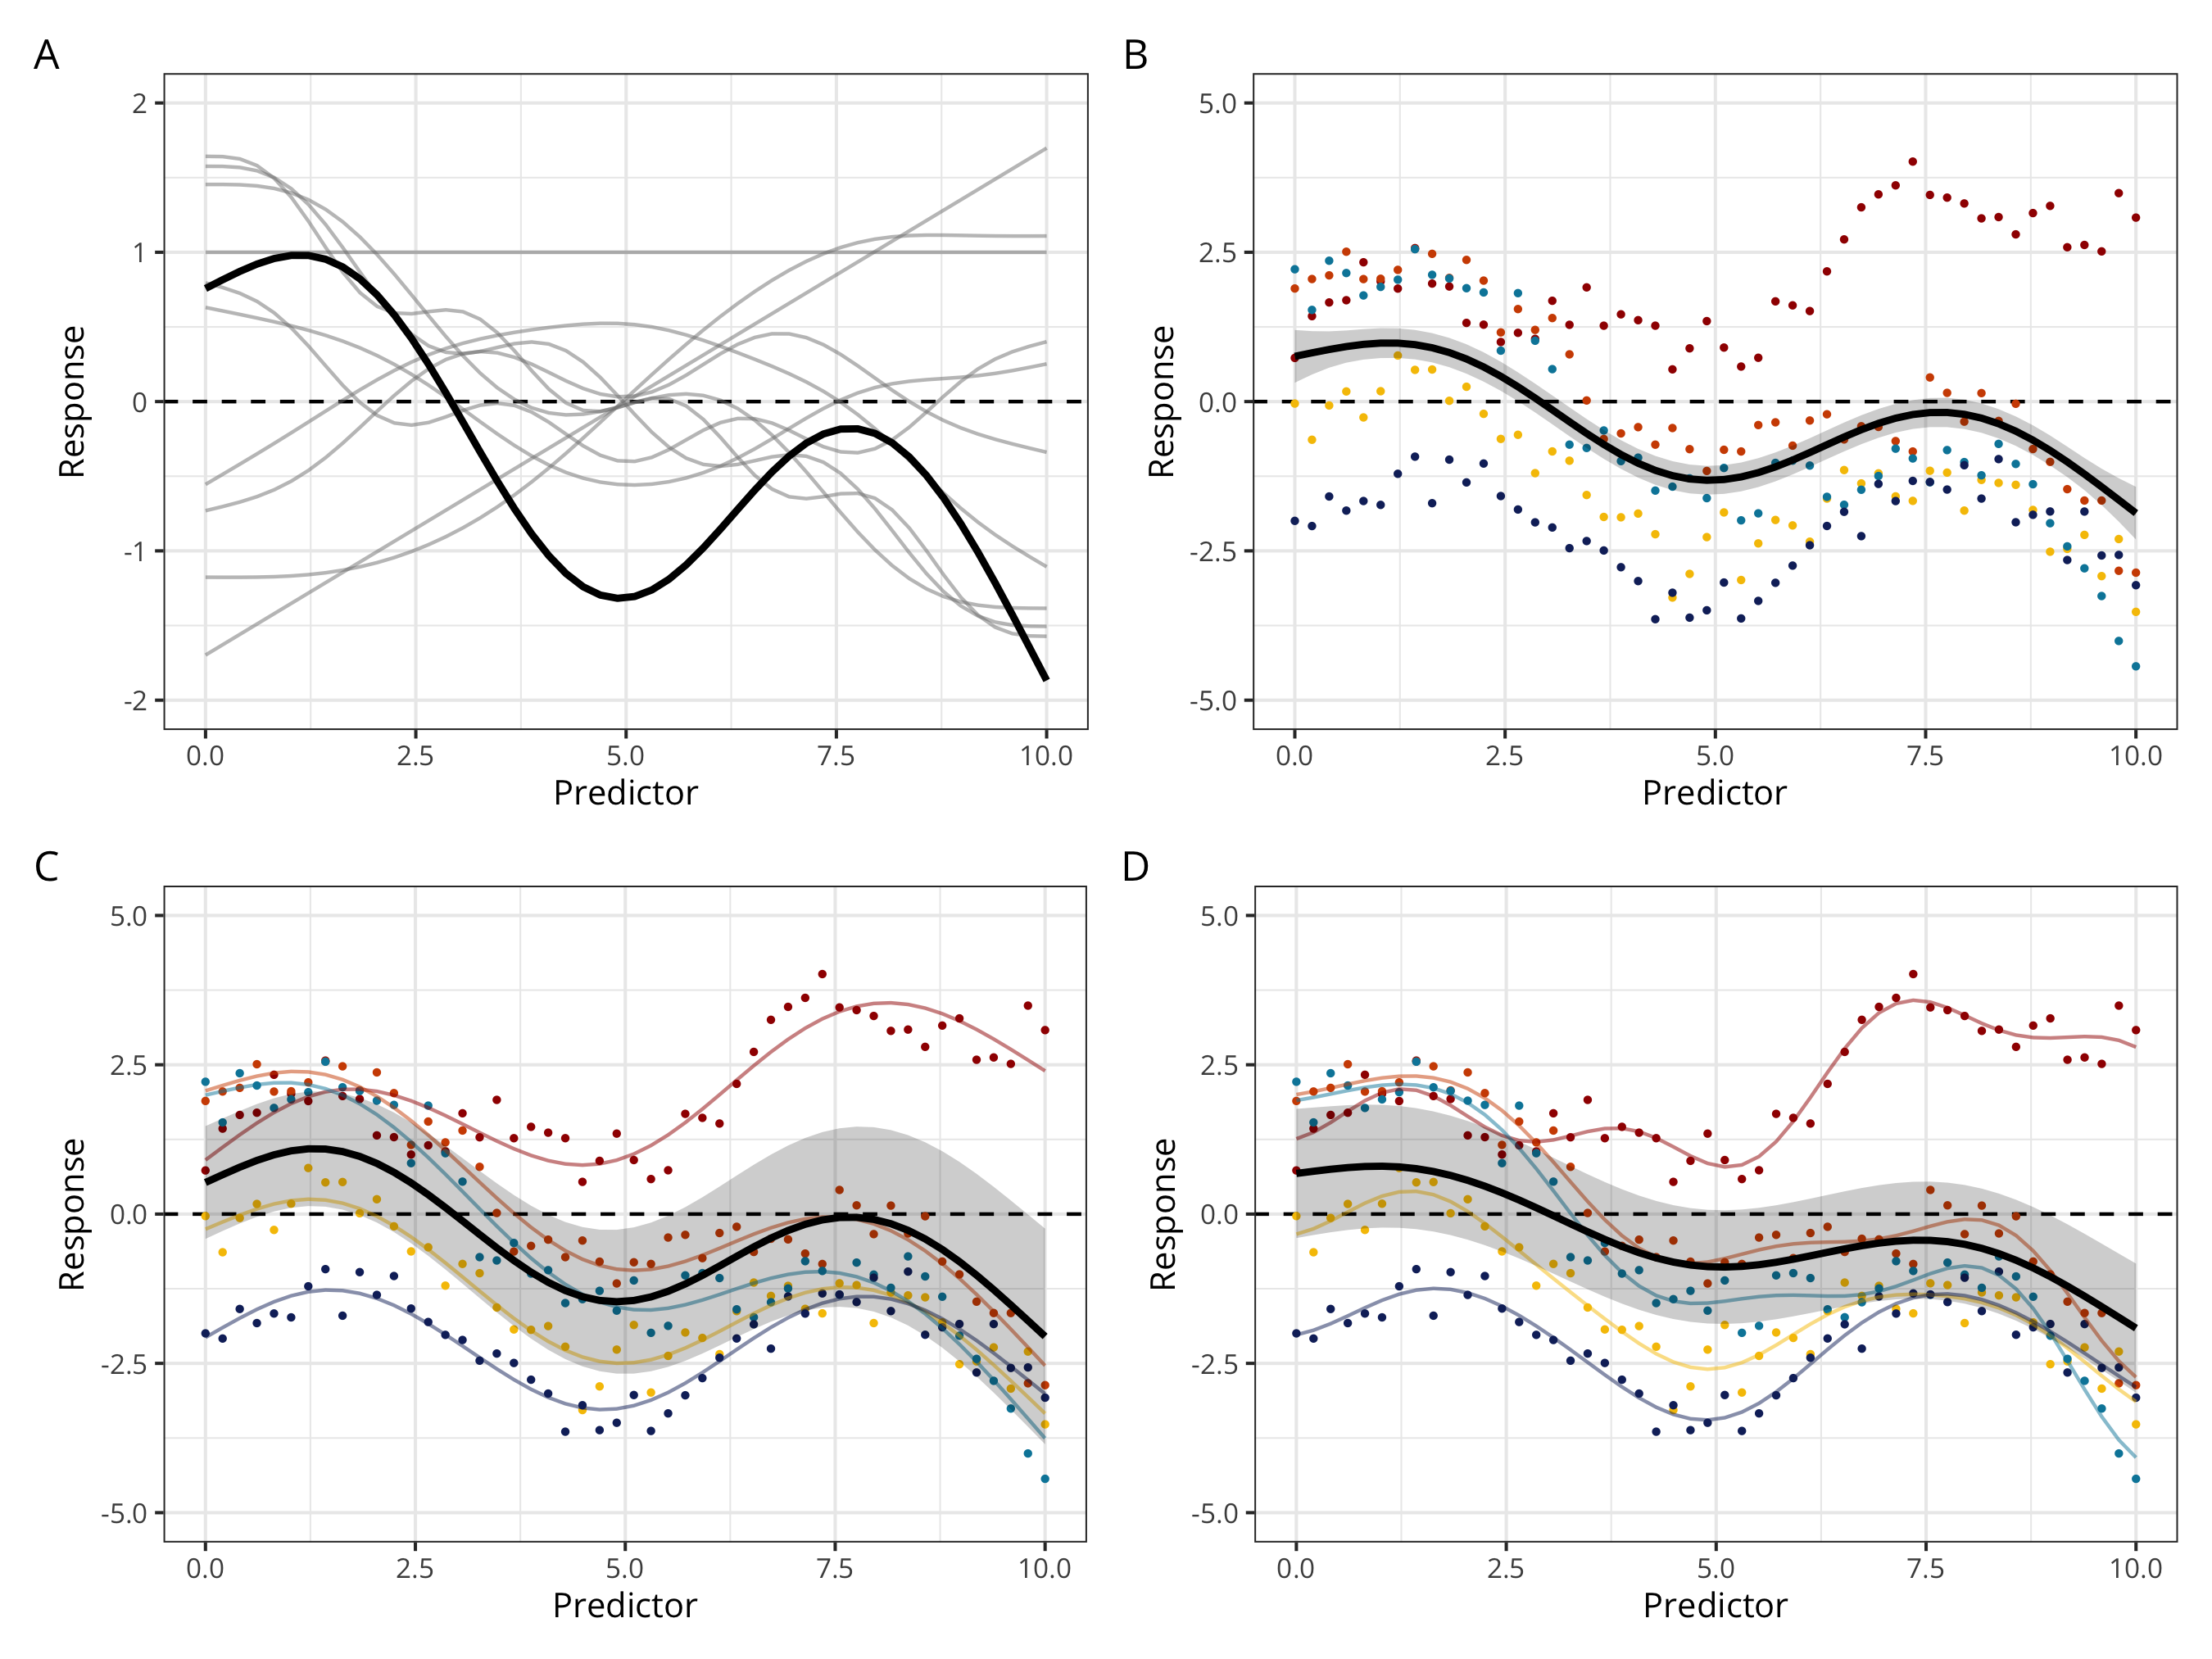
\includegraphics[width=1\textwidth,height=\textheight]{brms_meeg_files/figure-pdf/fig-intro-gam-1.png}

}

\end{figure}%

See Figure~\ref{fig-intro-gam}\ldots{} Introduction to multilevel GAMs
(\citeproc{ref-pedersen_hierarchical_2019}{E. J. Pedersen et al.,
2019})\ldots{} Now describe the Bayesian GAMM
(\citeproc{ref-miller2025}{Miller, 2025})\ldots{} Proper inclusion of
varying/random effects in the model specification protects against
overly wiggly curves (\citeproc{ref-baayen2020}{Baayen \& Linke,
2020})\ldots{} Generalising to scale and shape or ``distributional
GAMs'' (\citeproc{ref-rigby2005}{Rigby \& Stasinopoulos, 2005};
\citeproc{ref-umlauf2018}{Umlauf et al., 2018}) and applied to
neuroimaging data (\citeproc{ref-dinga2021}{Dinga et al., 2021})\ldots{}

Instead of averaging, obtain the smooth ERP signal from multilevel
GAM\ldots{} less susceptible to outliers
(\citeproc{ref-meulman2023}{Meulman et al., 2023})\ldots{}

\subsection{Objectives}\label{objectives}

Given the previously reported limitations of conventional methods to
precisely identify the onset and offset of M/EEG effects (e.g., ERPs,
decoding performance), we developed a model-based approach for
estimating the onset and offset of such effects. To achieve this, we
leveraged Bayesian generalised additive multilevel models (BGAMMs)
fitted in \texttt{R} via the \texttt{brms} package and compared the
performance of this approach to conventional methods on both simulated
and actual M/EEG data.

\section{Methods}\label{methods}

\subsection{M/EEG data simulation}\label{meeg-data-simulation}

Following the approach of Sassenhagen \& Draschkow
(\citeproc{ref-sassenhagen2019}{2019}) and Rousselet
(\citeproc{ref-rousselet_using_2025}{2025}), we simulated EEG data
stemming from two conditions, one with noise only, and the other with
noise + signal. As in previous studies, the noise was generated by
superimposing 50 sinusoids at different frequencies, following an
EEG-like spectrum (see code in the online supplementary materials and
details in \citeproc{ref-yeung2004}{Yeung et al., 2004}). As in
Rousselet (\citeproc{ref-rousselet_using_2025}{2025}), the signal was
generated from a truncated Gaussian distribution with an objective onset
at 160 ms, a peak at 250 ms, and an offset at 342 ms. We simulated this
signal for 250 timesteps between 0 and 0.5s, akin to a 500 Hz sampling
rate. We simulated data for a group of 20 participants (with variable
true onset) with 50 trials per participant and condition
(Figure~\ref{fig-eeg}).

\begin{figure}[!htb]

\caption{\label{fig-eeg}Mean simulated EEG activity in two conditions
with 50 trials each, for a group of 20 participants. The error band
represents the mean +/- 1 standard error of the mean.}

\centering{

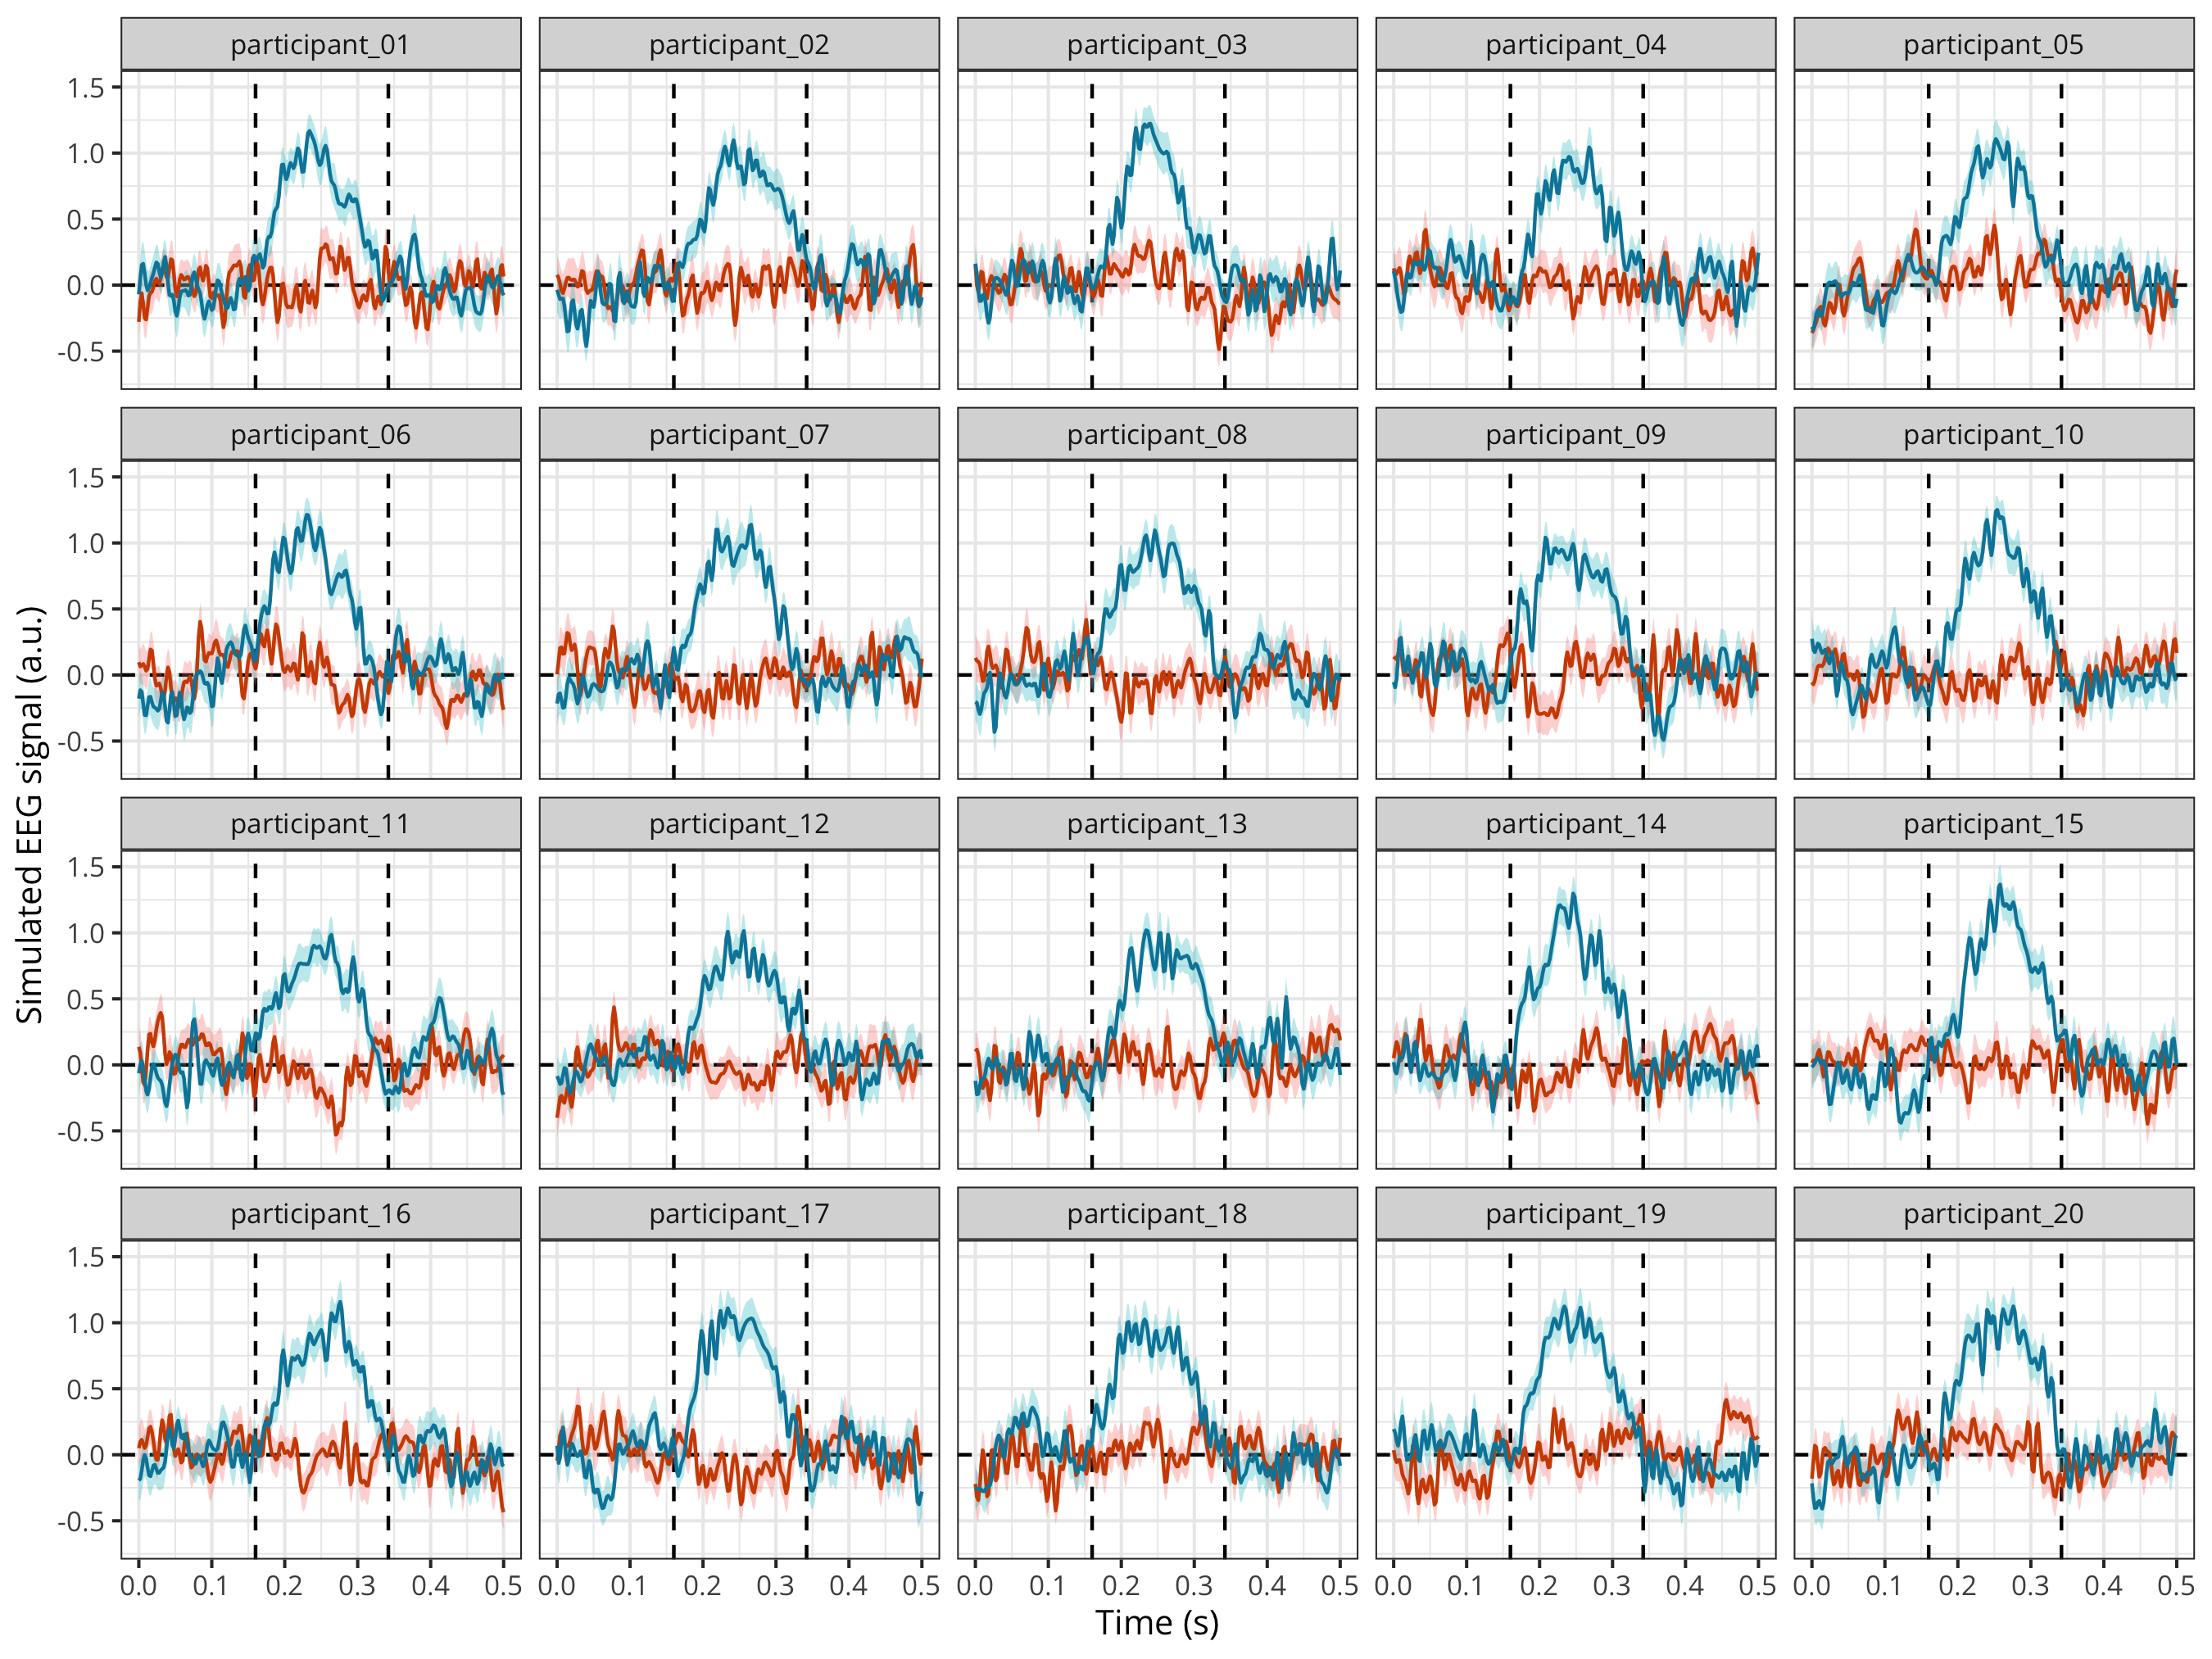
\includegraphics[width=1\textwidth,height=\textheight]{brms_meeg_files/figure-pdf/fig-eeg-1.png}

}

\end{figure}%

\subsection{Model description and model
fitting}\label{model-description-and-model-fitting}

We then fitted a Bayesian GAM (BGAM) using the \texttt{brms} package
(\citeproc{ref-brms2017}{Bürkner, 2017}, \citeproc{ref-brms2018}{2018};
\citeproc{ref-nalborczyk2019}{Nalborczyk et al., 2019}). We used the
default priors in \texttt{brms} (i.e., weakly informative priors). We
ran eight Markov Chain Monte-Carlo (MCMC) to approximate the posterior
distribution, including each 5000 iterations and a warmup of 2000
iterations, yielding a total of \(8 \times (5000-2000) = 24000\)
posterior samples to use for inference. Posterior convergence was
assessed examining trace plots as well as the Gelman--Rubin statistic
\(\hat{R}\) (\citeproc{ref-gabry2019}{Gabry et al., 2019};
\citeproc{ref-gelman2020}{Gelman et al., 2020}). The \texttt{brms}
package uses the same syntax as the \texttt{R} package \texttt{mgcv} v
1.9-1 (\citeproc{ref-mgcv}{Wood, 2017b}) for specifying smooth effects.
Figure~\ref{fig-plot-post-slope} shows the predictions of this model
together with the raw data.

\begin{Shaded}
\begin{Highlighting}[]
\CommentTok{\# averaging across participants}
\NormalTok{ppt\_df }\OtherTok{\textless{}{-}}\NormalTok{ raw\_df }\SpecialCharTok{\%\textgreater{}\%}
    \FunctionTok{group\_by}\NormalTok{(participant, condition, time) }\SpecialCharTok{\%\textgreater{}\%}
    \FunctionTok{summarise}\NormalTok{(}\AttributeTok{eeg =} \FunctionTok{mean}\NormalTok{(eeg) ) }\SpecialCharTok{\%\textgreater{}\%}
    \FunctionTok{ungroup}\NormalTok{()}

\CommentTok{\# defining a contrast for condition}
\FunctionTok{contrasts}\NormalTok{(ppt\_df}\SpecialCharTok{$}\NormalTok{condition) }\OtherTok{\textless{}{-}} \FunctionTok{c}\NormalTok{(}\SpecialCharTok{{-}}\FloatTok{0.5}\NormalTok{, }\FloatTok{0.5}\NormalTok{)}

\CommentTok{\# fitting the BGAM}
\NormalTok{gam }\OtherTok{\textless{}{-}} \FunctionTok{brm}\NormalTok{(}
    \CommentTok{\# thin{-}plate regression splines with k{-}1 basis functions}
\NormalTok{    eeg }\SpecialCharTok{\textasciitilde{}}\NormalTok{ condition }\SpecialCharTok{+} \FunctionTok{s}\NormalTok{(time, }\AttributeTok{bs =} \StringTok{"tp"}\NormalTok{, }\AttributeTok{k =} \DecValTok{20}\NormalTok{, }\AttributeTok{by =}\NormalTok{ condition),}
    \AttributeTok{data =}\NormalTok{ ppt\_df,}
    \AttributeTok{family =} \FunctionTok{gaussian}\NormalTok{(),}
    \AttributeTok{warmup =} \DecValTok{2000}\NormalTok{,}
    \AttributeTok{iter =} \DecValTok{5000}\NormalTok{,}
    \AttributeTok{chains =} \DecValTok{8}\NormalTok{,}
    \AttributeTok{cores =} \DecValTok{8}\NormalTok{,}
    \AttributeTok{file =} \StringTok{"models/gam.rds"}
\NormalTok{    )}
\end{Highlighting}
\end{Shaded}

However, the previous model only included constant (fixed) effects, thus
not properly accounting for between-participant variability. We next fit
a multilevel version of the BGAM (BGAMM, for an introduction to Bayesian
multilevel models in \texttt{brms}, see
\citeproc{ref-nalborczyk2019}{Nalborczyk et al., 2019}). Although it is
possible to fit a BGAMM at the single-trial level, we present a
computationally-lighter version of the model that is fitted directly on
by-participant summary statistics (mean and SD), similar to what is done
in meta-analysis.

\begin{Shaded}
\begin{Highlighting}[]
\CommentTok{\# averaging across participants}
\NormalTok{summary\_df }\OtherTok{\textless{}{-}}\NormalTok{ raw\_df }\SpecialCharTok{\%\textgreater{}\%}
    \FunctionTok{summarise}\NormalTok{(}
        \AttributeTok{eeg\_mean =} \FunctionTok{mean}\NormalTok{(eeg),}
        \AttributeTok{eeg\_sd =} \FunctionTok{sd}\NormalTok{(eeg),}
        \AttributeTok{.by =} \FunctionTok{c}\NormalTok{(participant, condition, time)}
\NormalTok{        )}

\CommentTok{\# defining a contrast for condition}
\FunctionTok{contrasts}\NormalTok{(summary\_df}\SpecialCharTok{$}\NormalTok{condition) }\OtherTok{\textless{}{-}} \FunctionTok{c}\NormalTok{(}\SpecialCharTok{{-}}\FloatTok{0.5}\NormalTok{, }\FloatTok{0.5}\NormalTok{)}

\CommentTok{\# fitting the BGAMM}
\NormalTok{meta\_gam }\OtherTok{\textless{}{-}} \FunctionTok{brm}\NormalTok{(}
    \CommentTok{\# using by{-}participant SD of ERPs across trials}
\NormalTok{    eeg\_mean }\SpecialCharTok{|} \FunctionTok{se}\NormalTok{(eeg\_sd) }\SpecialCharTok{\textasciitilde{}}
\NormalTok{        condition }\SpecialCharTok{+} \FunctionTok{s}\NormalTok{(time, }\AttributeTok{bs =} \StringTok{"cr"}\NormalTok{, }\AttributeTok{k =} \DecValTok{20}\NormalTok{, }\AttributeTok{by =}\NormalTok{ condition) }\SpecialCharTok{+}
\NormalTok{        (}\DecValTok{1} \SpecialCharTok{|}\NormalTok{ participant),}
    \AttributeTok{data =}\NormalTok{ summary\_df,}
    \AttributeTok{family =} \FunctionTok{gaussian}\NormalTok{(),}
    \AttributeTok{warmup =} \DecValTok{2000}\NormalTok{,}
    \AttributeTok{iter =} \DecValTok{5000}\NormalTok{,}
    \AttributeTok{chains =} \DecValTok{8}\NormalTok{,}
    \AttributeTok{cores =} \DecValTok{8}\NormalTok{,}
    \AttributeTok{file =} \StringTok{"models/meta\_gam.rds"}
\NormalTok{    )}

\CommentTok{\# fitting the BGAMM}
\CommentTok{\# meta\_gamm \textless{}{-} brm(}
\CommentTok{\#     \# using by{-}participant SD of ERPs across trials}
\CommentTok{\#     eeg\_mean | se(eeg\_sd) \textasciitilde{} condition +}
\CommentTok{\#         s(participant, bs = "re") +}
\CommentTok{\#         s(time, participant, bs = "fs", by = condition, m = 1),}
\CommentTok{\#     data = summary\_df,}
\CommentTok{\#     family = gaussian(),}
\CommentTok{\#     warmup = 2000,}
\CommentTok{\#     iter = 5000,}
\CommentTok{\#     chains = 8,}
\CommentTok{\#     cores = 8,}
\CommentTok{\#     control = list(adapt\_delta = 0.95),}
\CommentTok{\#     file = "models/meta\_gamm.rds"}
\CommentTok{\#     )}
\end{Highlighting}
\end{Shaded}

We depict the posterior predictions together with the posterior estimate
of the slope for \texttt{condition} at each timestep
(Figure~\ref{fig-plot-post-slope}). This figure suggests that the BGAMM
provides an adequate description of the simulated data (see further
posterior predictive checks in Section~\ref{sec-basis}).

\begin{figure}[!htb]

\caption{\label{fig-plot-post-slope}Posterior estimate of the EEG
activity in each condition (left) and posterior estimate of the
difference in EEG activity (right) according to the BGAMM.}

\centering{

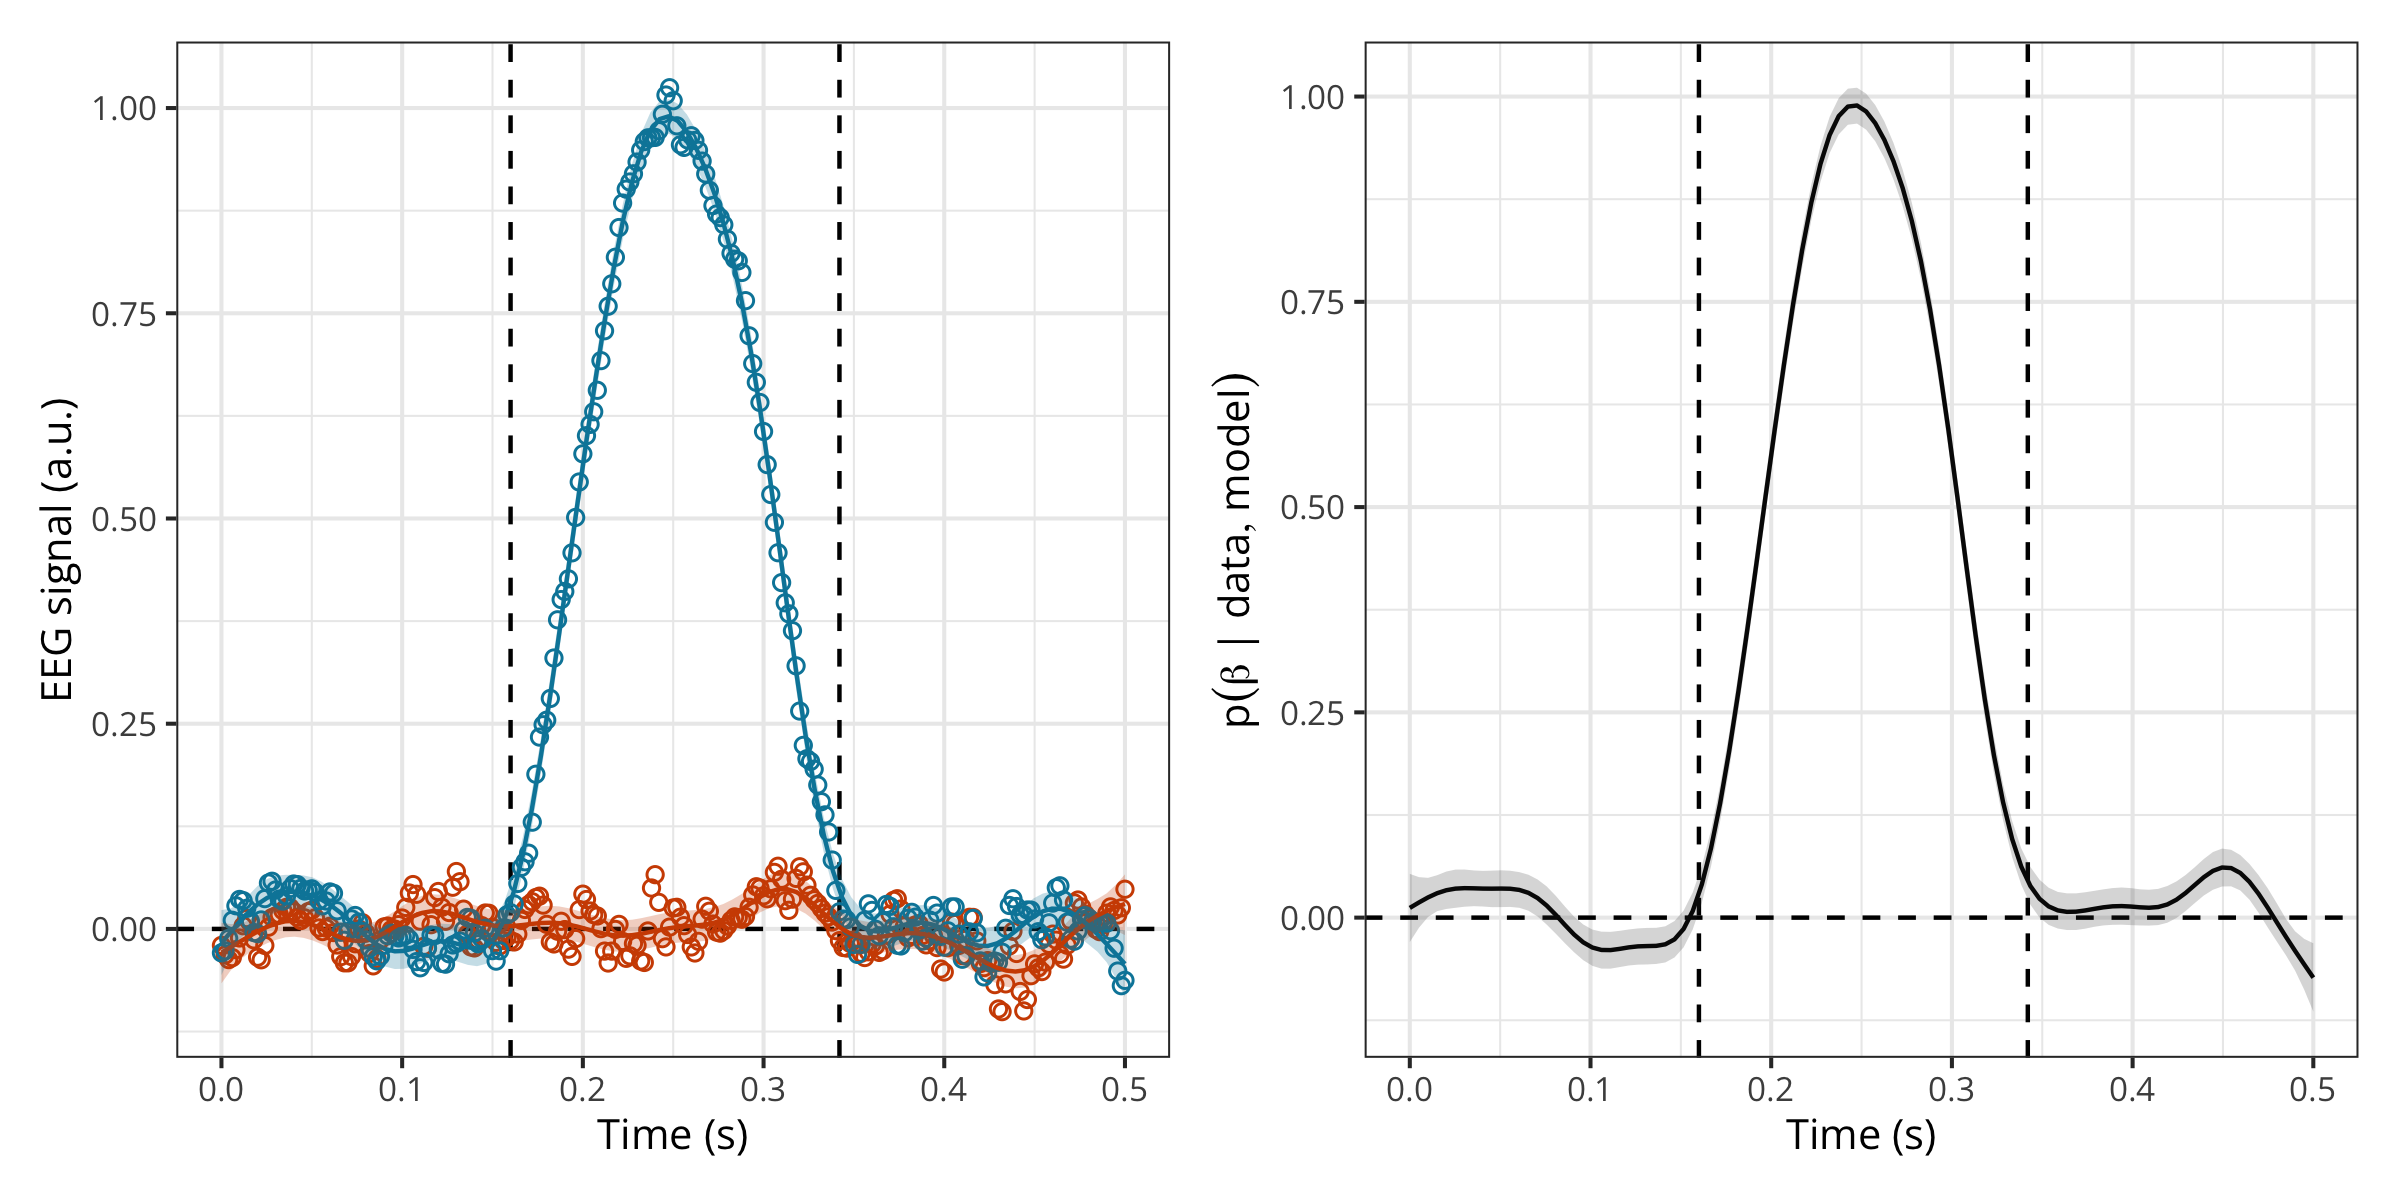
\includegraphics[width=1\textwidth,height=\textheight]{brms_meeg_files/figure-pdf/fig-plot-post-slope-1.png}

}

\end{figure}%

We then compute the posterior probability of the slope for
\texttt{condition} being above \(0\) (Figure~\ref{fig-post-prob-ratio},
left). From this quantity, we then compute the ratio of posterior
probabilities (i.e., \(p/(1-p)\)) and visualise the timecourse of this
ratio superimposed with the conventional thresholds on evidence ratios
(Figure~\ref{fig-post-prob-ratio}, right). Note that a ratio of 10 means
that the probability of the difference being above 0 is 10 times higher
than the probability of the difference not being above 0, given the
data, the priors, and other model's assumptions. Thresholding the
posterior probability ratio thus provides a model-based approach for
estimating the onset and offset of M/EEG effects. An important advantage
is that the proposed approach can be extended to virtually any model
structure. Moreover, the approach provides both group-level and
individual-level onset and offset estimates of M/EEG effects.

\begin{figure}[!htb]

\caption{\label{fig-post-prob-ratio}Left: Posterior probability of the
EEG difference (slope) being above 0 according to the BGAMM. Right:
Ratio of posterior probability according to the BGAMM (on a log10
scale). Timesteps above threshold (10) are highlighted in green. NB: the
minimum and maximum possible ratio values are determined (bounded) by
the number of available posterior samples in the model.}

\centering{

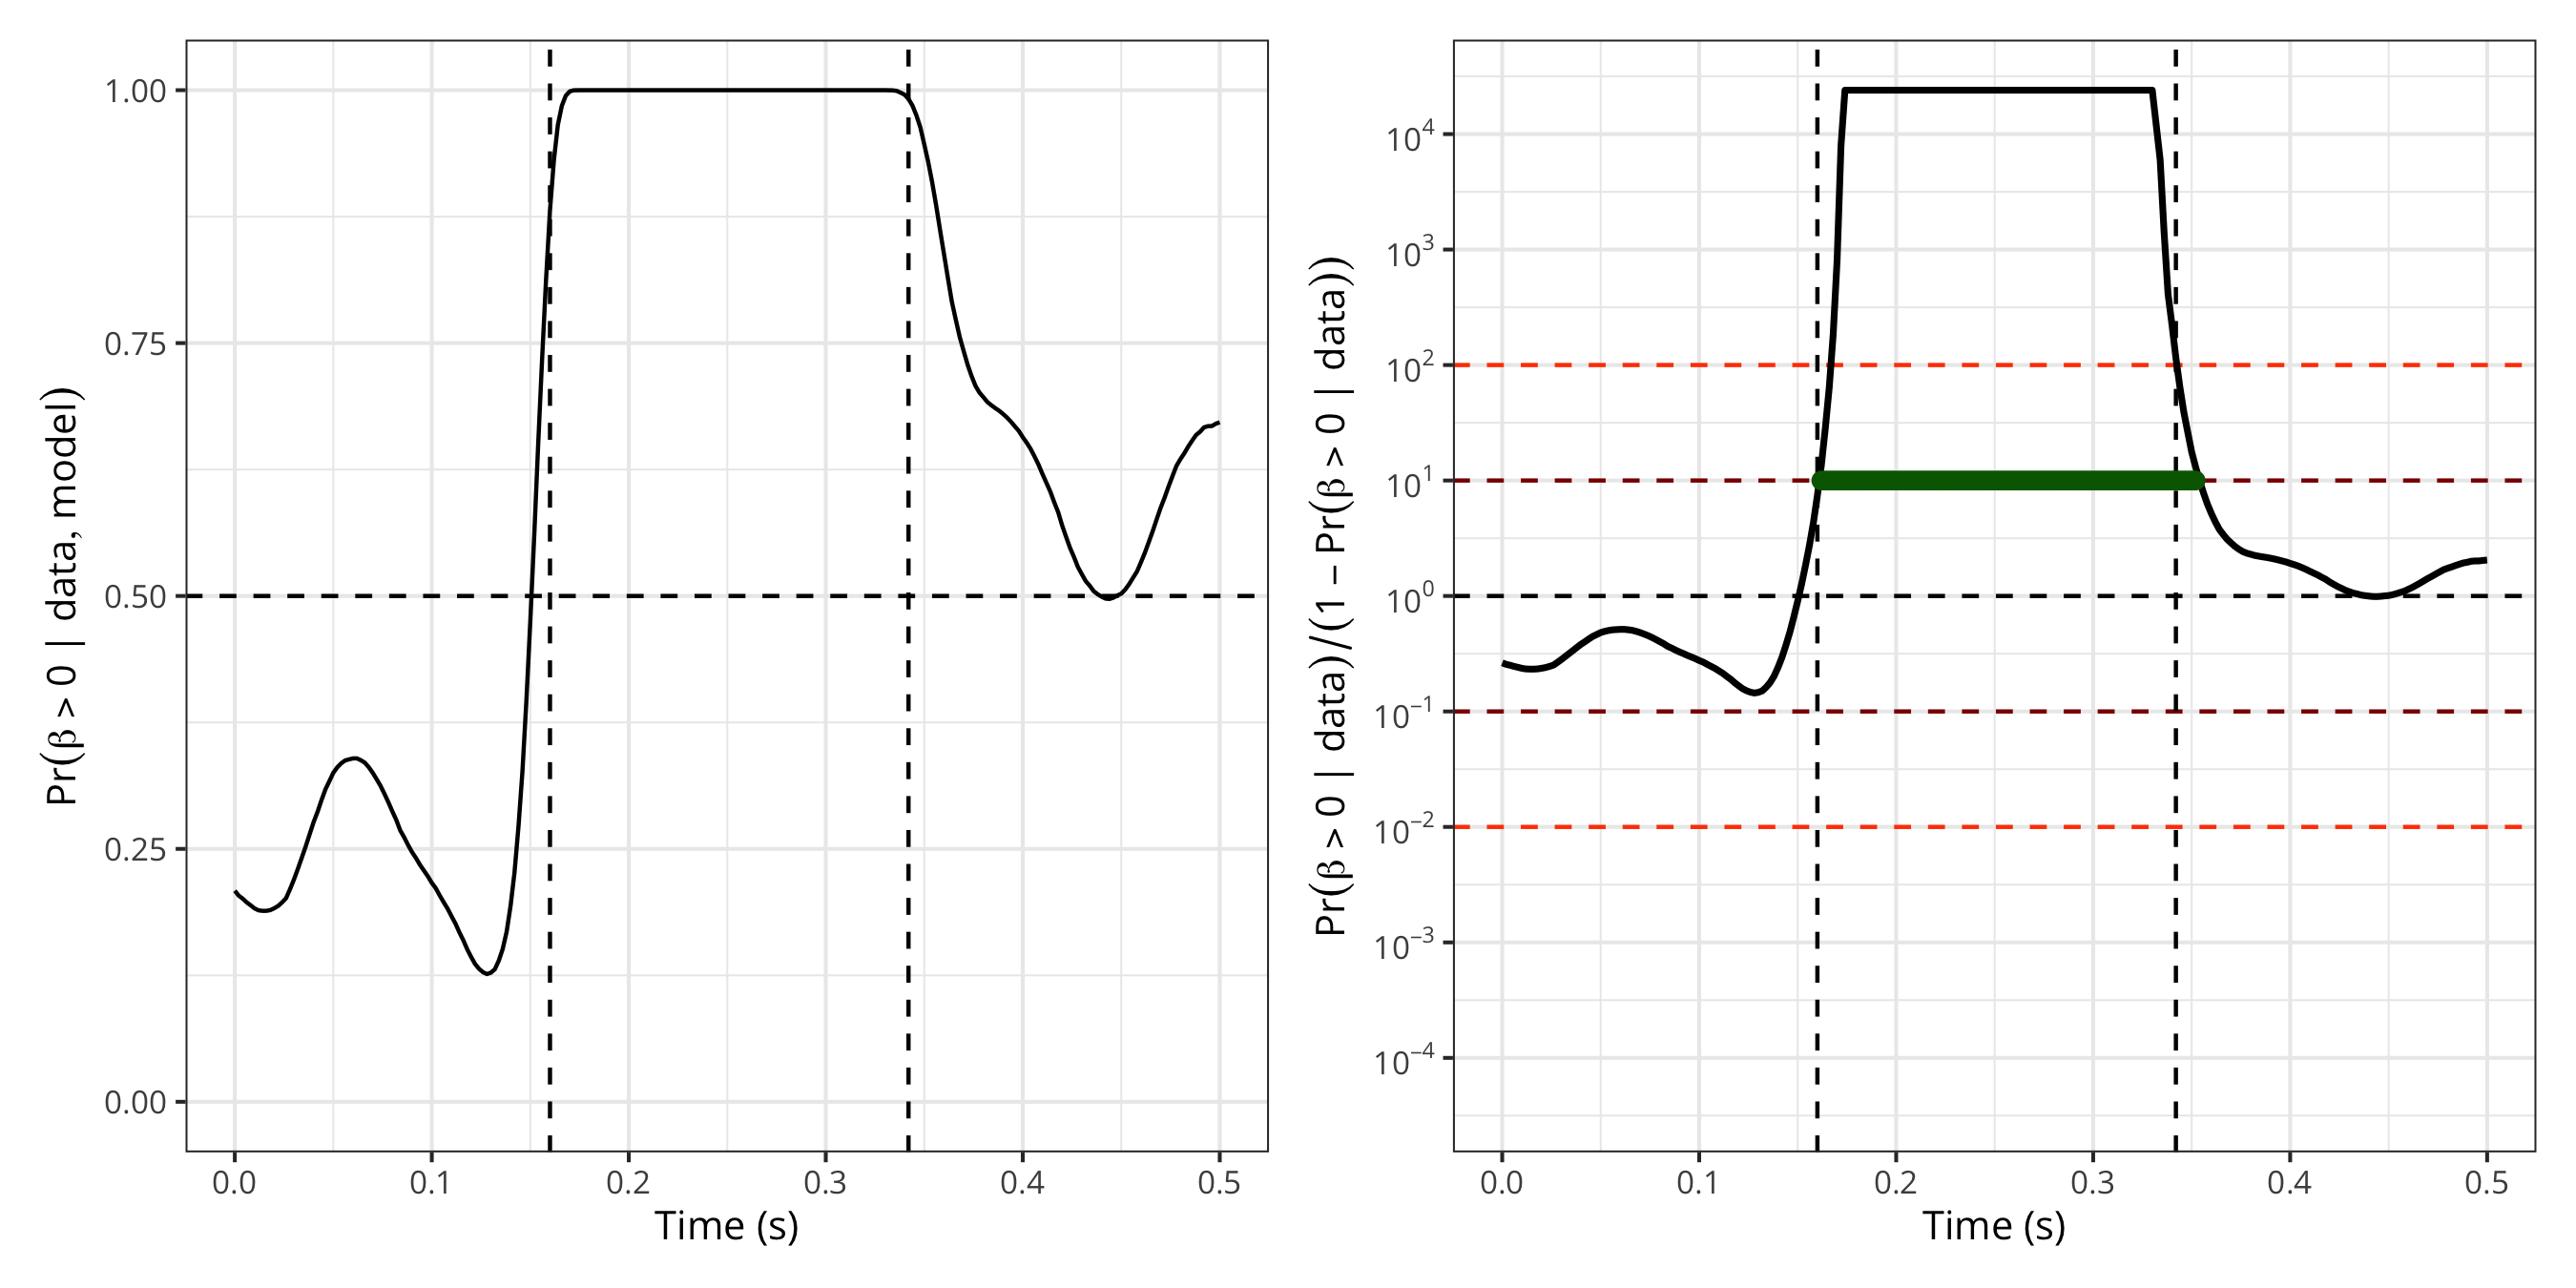
\includegraphics[width=1\textwidth,height=\textheight]{brms_meeg_files/figure-pdf/fig-post-prob-ratio-1.png}

}

\end{figure}%

\newpage

\subsection{Error properties of the proposed
approach}\label{error-properties-of-the-proposed-approach}

We then assess the performance of the proposed approach by computing the
difference between the true and estimated onset/offset of the EEG
difference according to various \texttt{k} (BGAM basis dimension) and
\texttt{threshold} values. Remember that the EEG signal was generated
from a truncated Gaussian with an objective onset at 160 ms, a maximum
at 250 ms, and an offset at 342 ms. Figure~\ref{fig-onset-error} shows
that the multilevel GAM can almost exactly recover the true onset and
offset values, given some reasonable choice of \texttt{k} and
\texttt{threshold} values. We provide more detailed recommendations on
how to set \texttt{k} in Section~\ref{sec-basis}. This figure further
reveals that the optimal \texttt{k} and \texttt{threshold} values may
differ for the onset and offset values, and there there seems to exist a
trade-off between these two parameters: lower \texttt{k} values lead to
poorer estimations, but these poor estimations can be compensated (only
to some extent) by higher \texttt{threshold} values (and reciprocally).

\begin{figure}[!htb]

\caption{\label{fig-onset-error}Average estimation error (RMSE) for the
onset (left) and offset (right) according to various basis dimension and
threshold values for the BGAM (computed from 100 simulated datasets).}

\centering{

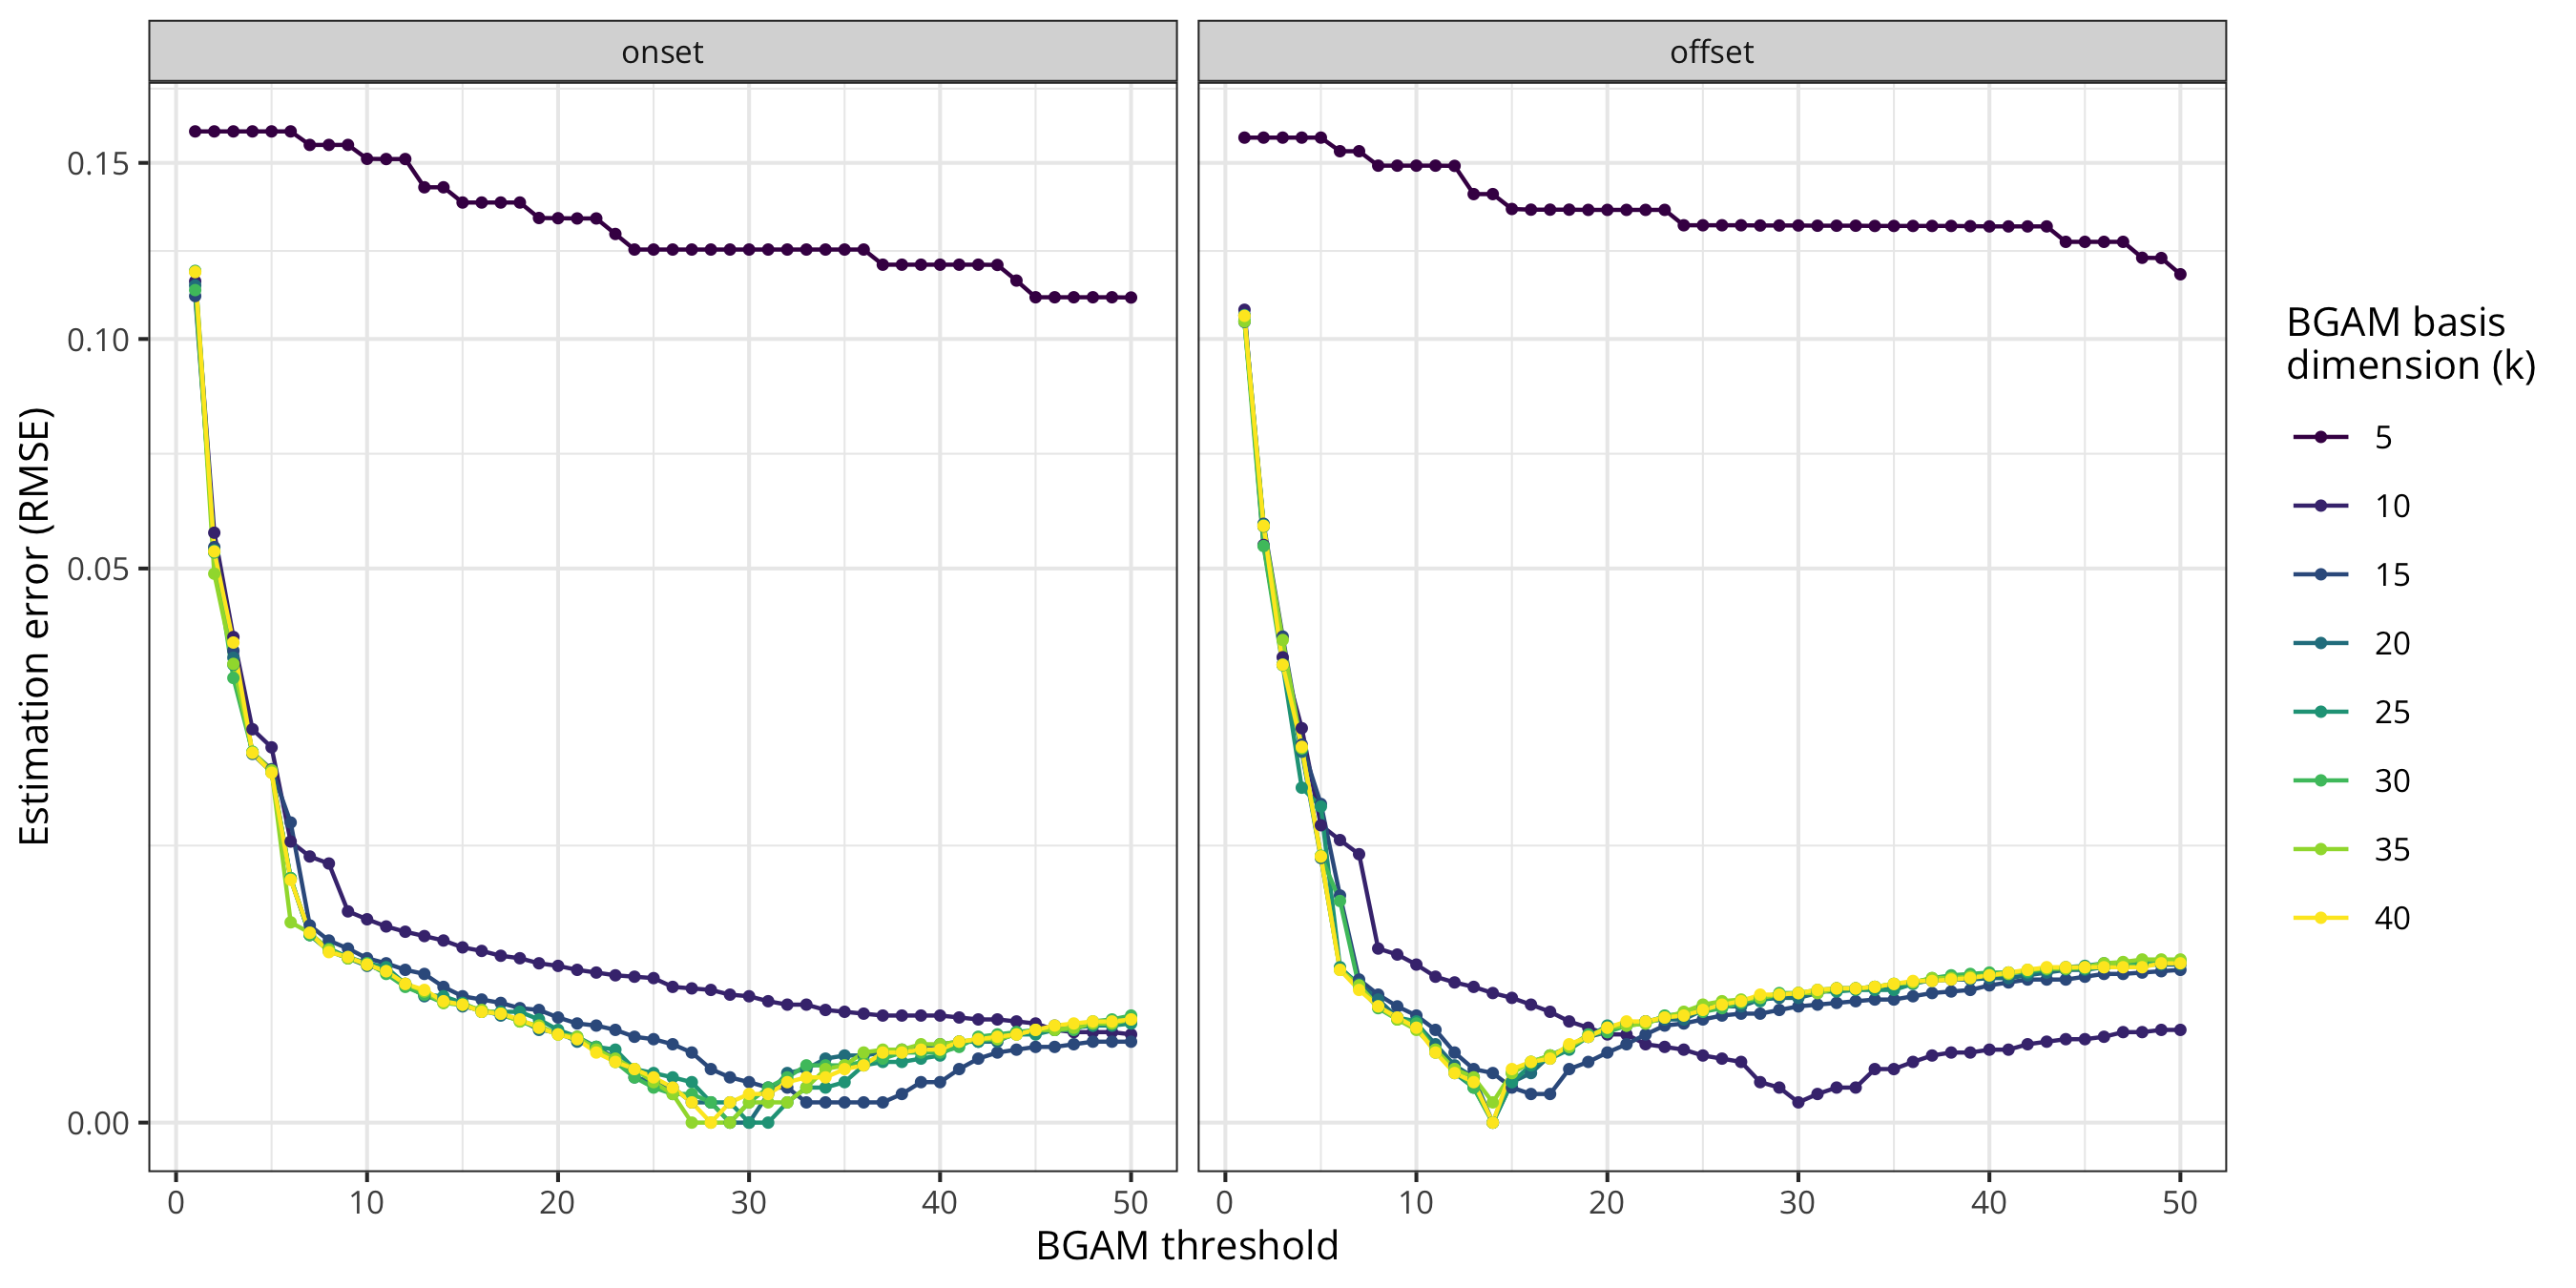
\includegraphics[width=1\textwidth,height=\textheight]{brms_meeg_files/figure-pdf/fig-onset-error-1.png}

}

\end{figure}%

\newpage

\subsection{Comparing the onsets/offsets estimates from other
approaches}\label{comparing-the-onsetsoffsets-estimates-from-other-approaches}

We then compared the ability of the BGAMM to accurately estimate the
onset and offset of the ERP difference to other widely-used methods.
First, we conducted mass-univariate t-tests (thus treating each timestep
independently) and identified the onset and offset of the ERP difference
as the first and last values crossing an arbitrary significance
threshold (\(\alpha = 0.05\)). We then followed the same approach but
after applying different forms of multiplicity correction to the
\(p\)-values. We compared two methods that control the FDR (i.e.,
\texttt{BH95}, \citeproc{ref-benjamini1995}{Benjamini \& Hochberg,
1995}; and \texttt{BY01}, \citeproc{ref-benjamini2001}{Benjamini \&
Yekutieli, 2001}), one method that controls the FWER (i.e.,
Holm--Bonferroni method, \citeproc{ref-holm1979}{Holm, 1979}), and two
cluster-based permutation methods (permutation with a single
cluster-forming threshold and threshold-free cluster enhancement,
\texttt{TFCE}, \citeproc{ref-smith2009}{S. Smith \& Nichols, 2009}). The
\texttt{BH95}, \texttt{BY01}, and \texttt{Holm} corrections were applied
to the p-values using the \texttt{p.adjust()} function in \texttt{R}.
The cluster-based inference was implemented using a cluster-sum
statistic of squared \(t\)-values, as implemented in \texttt{MNE-Python}
(\citeproc{ref-gramfort2013}{Gramfort, 2013}), called via the \texttt{R}
package \texttt{reticulate} v 1.42.0 (\citeproc{ref-reticulate}{Ushey et
al., 2024}). We also compared these estimates to the onset and offset as
estimated using the binary segmentation algorithm, as implemented in the
\texttt{R} package \texttt{changepoint} v 2.3
(\citeproc{ref-changepoint}{Killick et al., 2022}), and applied directly
to the squared \(t\)-values (as in
\citeproc{ref-rousselet_using_2025}{Rousselet, 2025}).
Figure~\ref{fig-corrections} illustrates the onsets and offsets
estimated by each method on a single simulated dataset and shows that
all methods systematically overestimate the true onset and underestimate
the true offset.

\begin{figure}[!htb]

\caption{\label{fig-corrections}Exemplary timecourse of squared t-values
with true onset and offset (vertical black dashed lines) and
onsets/offsets identified using the raw p-values, the corrected p-values
(BH95, BY01, Holm), the cluster-based methods (Cluster mass, TFCE), or
using the binary segmentation method (Change point).}

\centering{

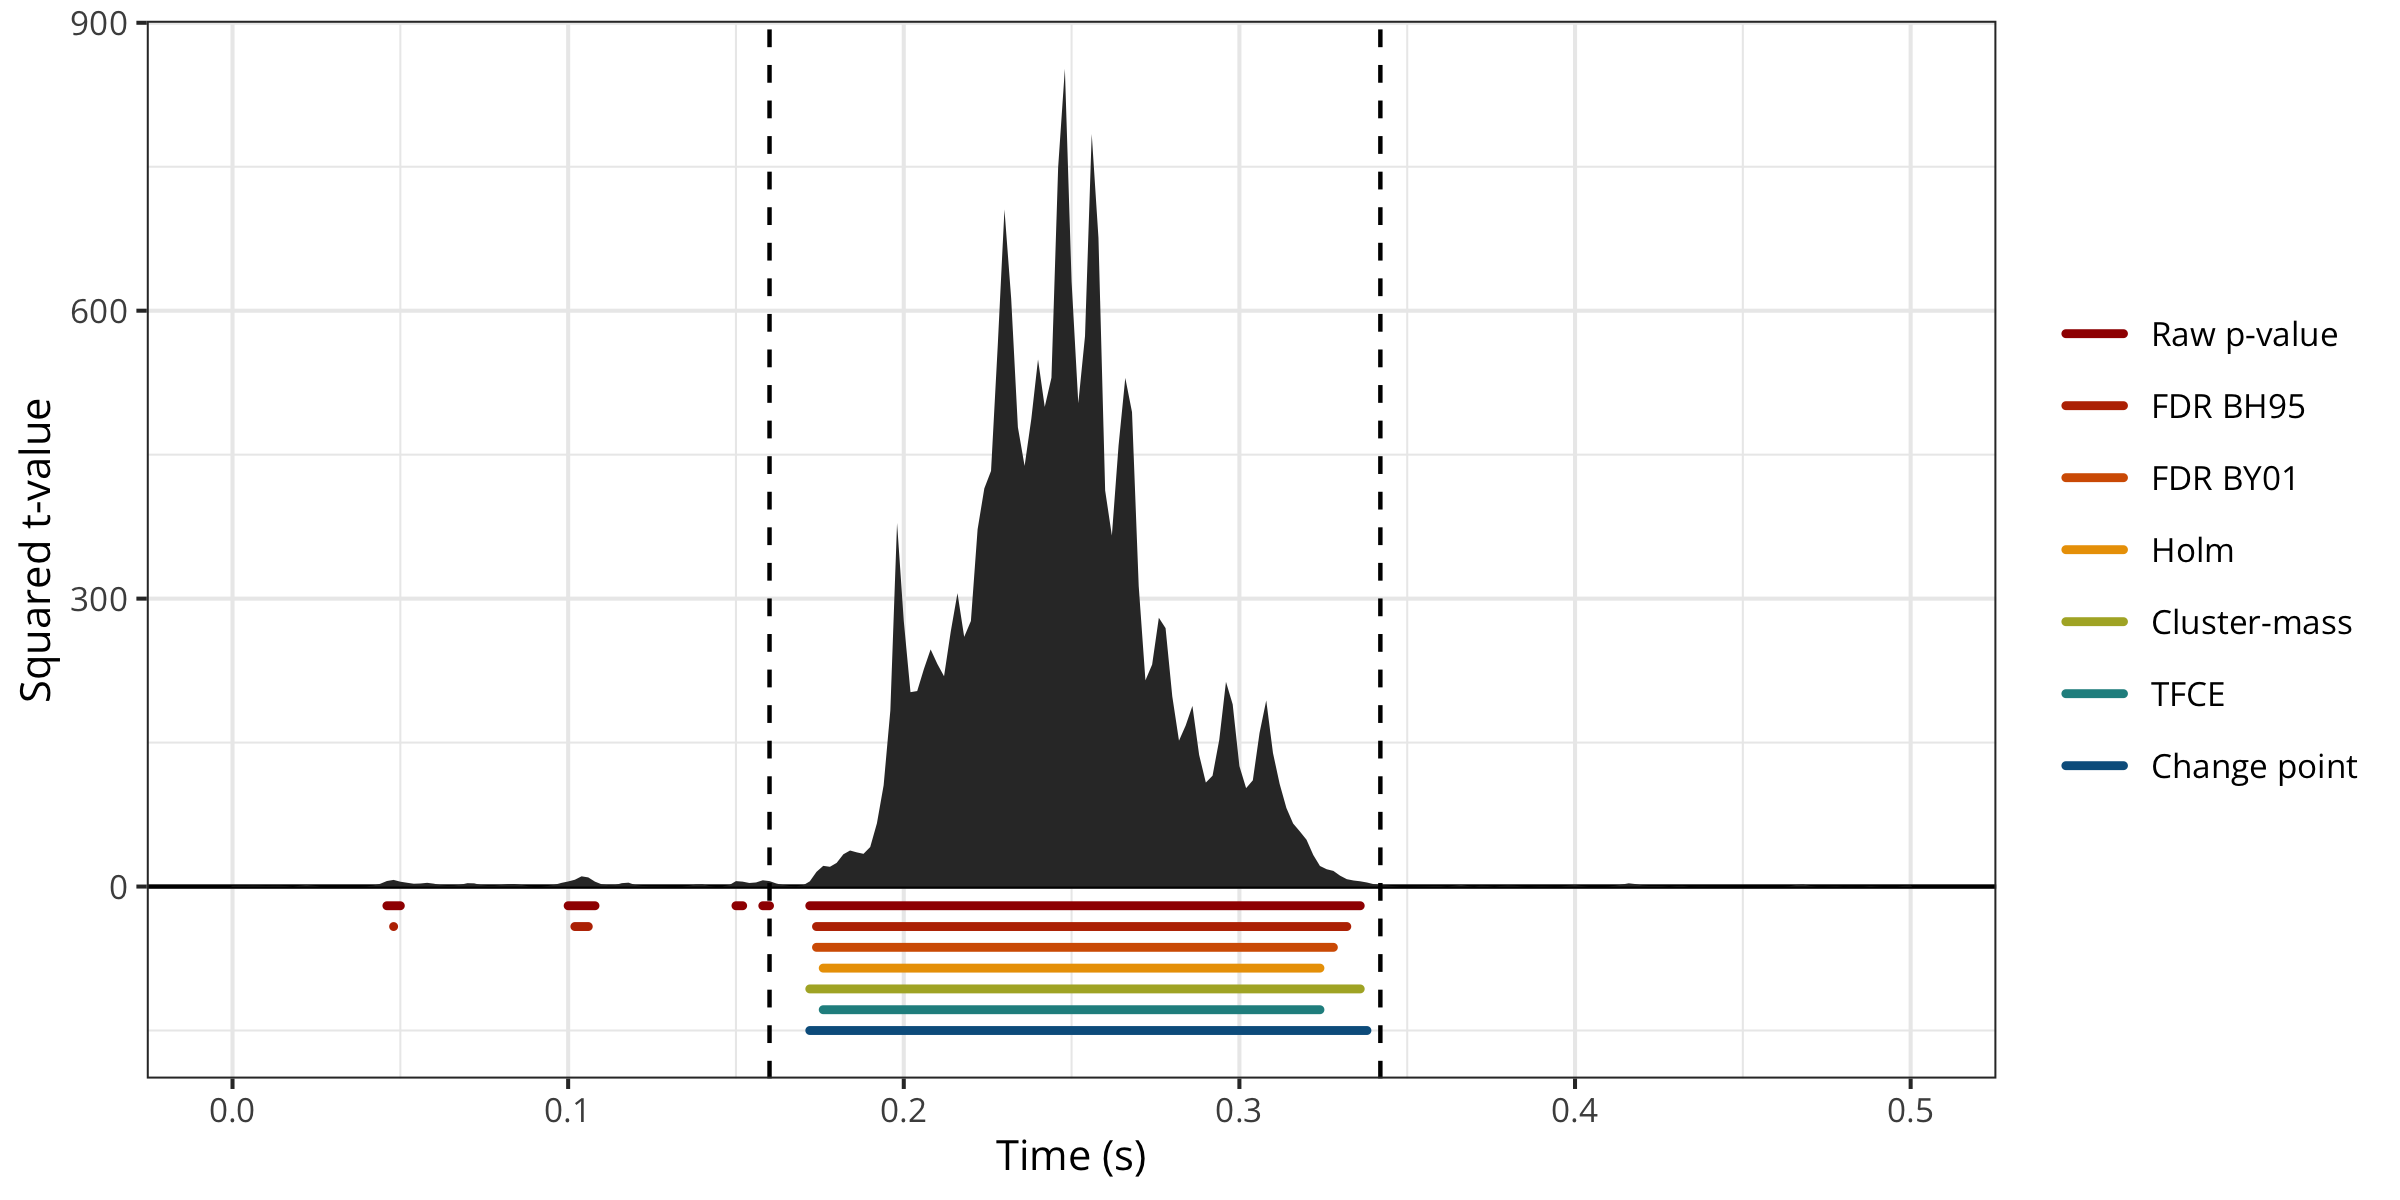
\includegraphics[width=1\textwidth,height=\textheight]{brms_meeg_files/figure-pdf/fig-corrections-1.png}

}

\end{figure}%

\newpage

\subsection{Simulation study}\label{simulation-study}

To assess the accuracy of group-level onset estimation, the various
methods were compared using the bias (i.e., median(estimated-true)),
median absolute error (MAE), root mean square error (RMSE), variance,
and median absolute deviation (MAD) of onset/offset estimates computed
on 1,000 simulated datasets. As in Rousselet
(\citeproc{ref-rousselet_using_2025}{2025}), each participant was
assigned a random onset between 150 and 170ms. Whereas the present
article focuses on one-dimensional signas (e.g., one M/EEG channel), we
provice a 2D application in Section~\ref{sec-2D}.

\subsection{Application to actual MEG
data}\label{application-to-actual-meg-data}

To complement the simulation study, we evaluated the performance of the
various methods on actual MEG data (decoding results from
\citeproc{ref-nalborczyk:inprep}{Nalborczyk et al., in preparation}). In
this study, we conducted time-resolved multivariate pattern analysis
(MVPA, also known as decoding) of MEG data during reading tasks. As a
result, we obtain a timecourse of decoding performance (ROC AUC),
bounded between 0 and 1, for each participant (\(N=32\)). Next, we
wanted to \emph{test} whether the group-level average decoding accuracy
is above chance (i.e., 0.5) at each timestep
(Figure~\ref{fig-decoding-data}). To achieve this, we fitted a BGAM as
introduced previously, but we replaced the \(\mathrm{Normal}\)
likelihood function by a \(\mathrm{Beta}\) one to account for the
bounded nature of AUC values (between 0 and 1) (for a tutorial on Beta
regression, see \citeproc{ref-coretta2025}{Coretta \& Bürkner, 2025}).

Note that although we chose a basis dimension of \(k=50\), which seems
appropriate for the present data, this choice should be adapted
according to the properties of the modelled data (e.g., signal-to-noise
ratio, prior low-pass filtering, sampling rate) and should be assessed
by the usual model checking tools (e.g., posterior predictive checks,
see also Section~\ref{sec-basis}). To better distinguish signal from
noise, we also defined a region of practical equivalence (ROPE,
\citeproc{ref-kruschke2017}{Kruschke \& Liddell, 2017}), defined as the
chance level plus the standard deviation of the (group-level average)
decoding performance during the baseline period.

\begin{Shaded}
\begin{Highlighting}[]
\CommentTok{\# fitting the Beta GAM}
\NormalTok{meg\_decoding\_gam }\OtherTok{\textless{}{-}} \FunctionTok{brm}\NormalTok{(}
\NormalTok{    auc }\SpecialCharTok{\textasciitilde{}} \FunctionTok{s}\NormalTok{(time, }\AttributeTok{bs =} \StringTok{"cr"}\NormalTok{, }\AttributeTok{k =} \DecValTok{50}\NormalTok{),}
    \AttributeTok{data =}\NormalTok{ decoding\_df,}
    \AttributeTok{family =} \FunctionTok{Beta}\NormalTok{(),}
    \AttributeTok{warmup =} \DecValTok{2000}\NormalTok{,}
    \AttributeTok{iter =} \DecValTok{5000}\NormalTok{,}
    \AttributeTok{chains =} \DecValTok{4}\NormalTok{,}
    \AttributeTok{cores =} \DecValTok{4}
\NormalTok{    )}
\end{Highlighting}
\end{Shaded}

We assessed the reliability of the proposed approach using a form of
permutation-based split-half reliability (as for instance in
\citeproc{ref-rosenblatt2018}{Rosenblatt et al., 2018}), which consisted
of the following steps. First, we created 1,000 split halves of the data
(i.e., with half the participants in the original data, that is, 16
participants). For each split, we estimated the onset/offset using all
methods described previously. Third, we summarised the distribution of
onset/offset estimates using the median ``error'' (i.e., difference
between the split estimate and the estimate obtained using the full
dataset) and the variance across splits. This approach allows assessing
how similar the estimate of each half split is to the full dataset (thus
acting as a proxy for the population) and how variable the estimates are
across split halves.

\begin{figure}[!htb]

\caption{\label{fig-decoding-data}Group-level average decoding
performance (N=32) superimposed with the GAM predictions (in blue) and
the region of practical equivalence (ROPE, in orange) computed from the
baseline period (data from \citeproc{ref-nalborczyk:inprep}{Nalborczyk
et al., in preparation}). The blue horizontal markers indicate the
timesteps at which the posterior probability ratio exceeds 20.}

\centering{

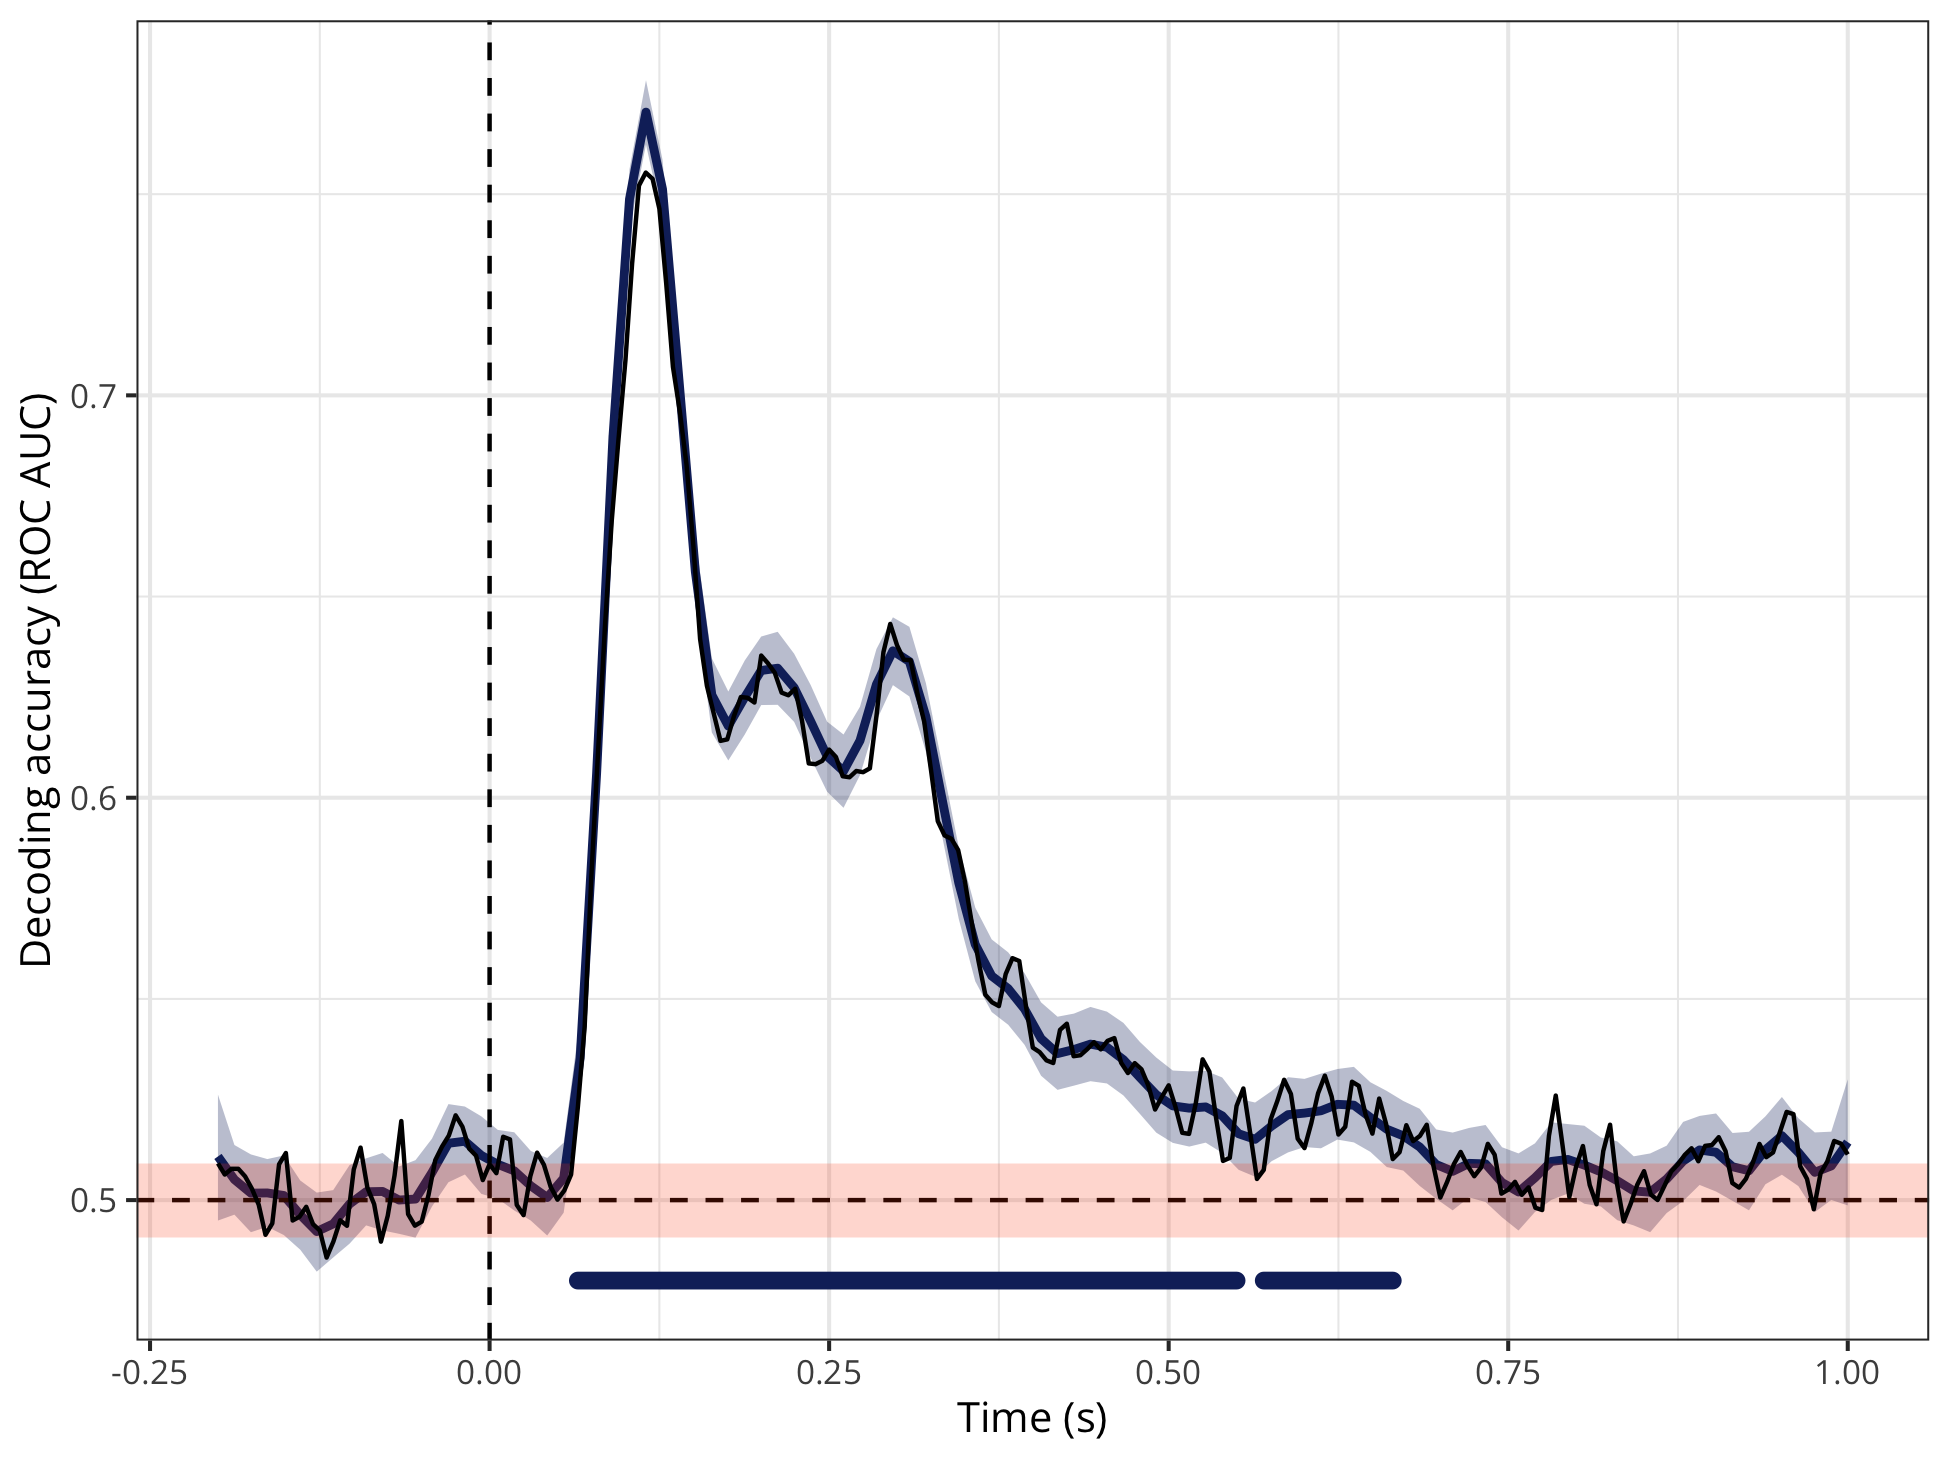
\includegraphics[width=0.75\textwidth,height=\textheight]{brms_meeg_files/figure-pdf/fig-decoding-data-1.png}

}

\end{figure}%

\newpage

\section{Results}\label{results}

This section is divided in two parts. First, we present the results from
the simulation study, assessing the bias and variance of each method
when applied to simulated data in which the ground truth is known.
Second, we present the results obtained when applying the different
methods to actual MEG data (decoding performance through time),
assessing the reliability of the estimates provided by each method.

\subsection{Simulation study (bias and
variance)}\label{simulation-study-bias-and-variance}

Figure~\ref{fig-simulation-results} shows a summary of the simulation
results, revealing that the proposed approach (\texttt{BGAM}) has the
lowest median absolute error (MAE) and variance for both the onset and
offset estimates. The \texttt{Cluster\ mass} and \texttt{Change\ point}
also have good performance, but surprisingly, the \texttt{TFCE} method
has relatively bad performance for estimating the effect offset (similar
performance to the \texttt{Holm} and \texttt{FDR\ BY01} methods).
Unsurprisingly, the \texttt{Raw\ p-value} and \texttt{FDR\ BH95} methods
show the worst performance.

\begin{figure}[!htb]

\caption{\label{fig-simulation-results}Median absolute error and
variance of onset and offset estimates for each method. Variance is
plotted on a log10 scale for visual purposes.}

\centering{

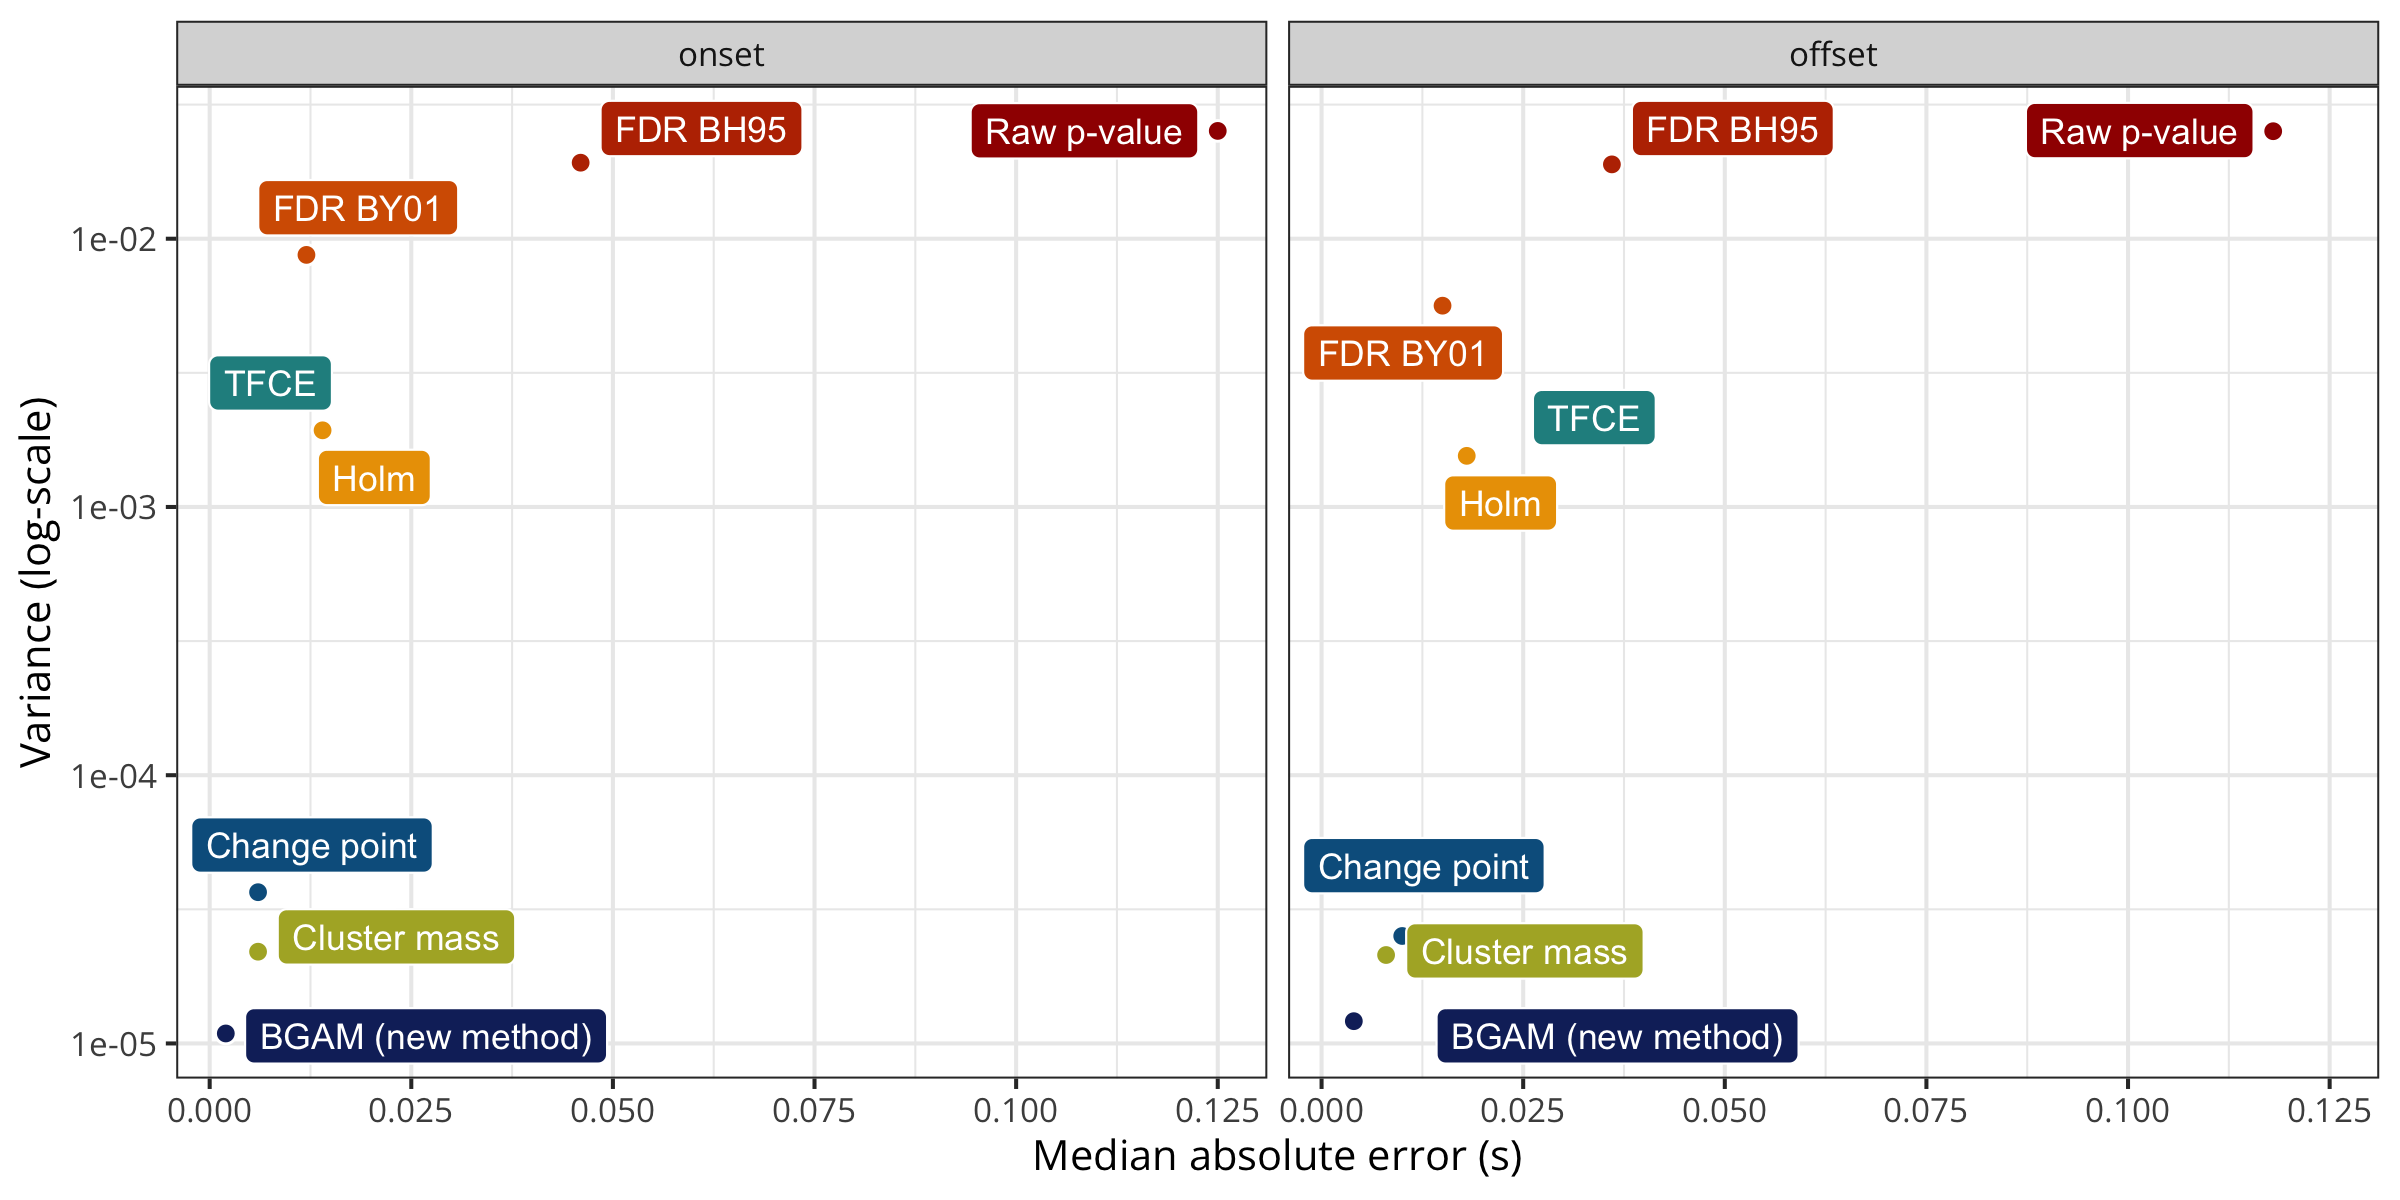
\includegraphics[width=1\textwidth,height=\textheight]{brms_meeg_files/figure-pdf/fig-simulation-results-1.png}

}

\end{figure}%

Results are further summarised in Table~\ref{tbl-simulation-results},
which shows that the \texttt{BGAM} is perfectly unbiased (i.e., it has a
bias of 0s) for the onset and almost exactly unbiased for the onset
(with a bias of approximately -2ms). The \texttt{Bias} column shows that
all other methods tend to estimate the onset later than the true onset
and to estimate the offet earlier than the true offset. As can be seen
from this table, the \texttt{BGAM} has the best performance on all
included metrics.

\begin{table}

{\caption{{Summary statistics of the onset and offset estimates for each
method (ordered by the absolute value of the
bias).}{\label{tbl-simulation-results}}}}

\fontsize{9.0pt}{10.8pt}\selectfont
\begin{tabular*}{\linewidth}{@{\extracolsep{\fill}}lccccc}
\toprule
 & Bias & MAE & RMSE & Variance & MAD \\ 
\midrule\addlinespace[2.5pt]
\multicolumn{6}{l}{onset} \\[2.5pt] 
\midrule\addlinespace[2.5pt]
BGAM (new method) & 0.0000 & 0.0020 & 0.0001 & 0.0000 & 0.0030 \\ 
Cluster mass & 0.0060 & 0.0060 & 0.0057 & 0.0000 & 0.0044 \\ 
Change point & 0.0060 & 0.0060 & 0.0051 & 0.0000 & 0.0059 \\ 
Raw p-value & 0.0060 & 0.1250 & 0.0711 & 0.0252 & 0.1942 \\ 
FDR BH95 & 0.0080 & 0.0460 & 0.0599 & 0.0192 & 0.0801 \\ 
FDR BY01 & 0.0120 & 0.0120 & 0.0443 & 0.0087 & 0.0059 \\ 
TFCE & 0.0140 & 0.0140 & 0.0270 & 0.0019 & 0.0059 \\ 
Holm & 0.0140 & 0.0140 & 0.0270 & 0.0019 & 0.0059 \\ 
\midrule\addlinespace[2.5pt]
\multicolumn{6}{l}{offset} \\[2.5pt] 
\midrule\addlinespace[2.5pt]
BGAM (new method) & -0.0020 & 0.0040 & 0.0021 & 0.0000 & 0.0030 \\ 
Cluster mass & -0.0080 & 0.0080 & 0.0084 & 0.0000 & 0.0059 \\ 
Raw p-value & -0.0080 & 0.1180 & 0.0725 & 0.0252 & 0.1868 \\ 
Change point & -0.0100 & 0.0100 & 0.0096 & 0.0000 & 0.0059 \\ 
FDR BH95 & -0.0100 & 0.0360 & 0.0578 & 0.0189 & 0.0682 \\ 
FDR BY01 & -0.0140 & 0.0150 & 0.0204 & 0.0056 & 0.0059 \\ 
TFCE & -0.0180 & 0.0180 & 0.0261 & 0.0016 & 0.0030 \\ 
Holm & -0.0180 & 0.0180 & 0.0262 & 0.0016 & 0.0030 \\ 
\bottomrule
\end{tabular*}

\end{table}

\newpage

\subsection{Application to actual MEG data
(reliability)}\label{application-to-actual-meg-data-reliability}

Figure~\ref{fig-onset-offset} shows the group-level average decoding
performance through time with onset and offset estimates from each
method. Overall, this figure shows that both the \texttt{Raw\ p-value}
and \texttt{FDR\ BH95} methods are extremely lenient, considering that
the decoding performance is above chance before the onset of the
stimulus (false positive) and until the end of the trial. The
\texttt{Change\ point} and \texttt{Cluster\ mass} methods seem the most
conservative methods, identifying a time window from approximately +60ms
to +500ms. The \texttt{Holm}, \texttt{TFCE}, and \texttt{BGAM} methods
produce similar estimates of onset and offset, ranging from
approximately +60ms to +650ms, although the \texttt{BGAM} method seems
to result in fewer clusters.\footnote{It should be noted that although
  each method can produce several ``clusters'' of timesteps, we only
  considered the first (onset) and last (offset) timesteps identified by
  each method to compute the estimation error.}

\begin{figure}[!htb]

\caption{\label{fig-onset-offset}Group-level average decoding
performance through time with onset and offset estimates for each method
(data from \citeproc{ref-nalborczyk:inprep}{Nalborczyk et al., in
preparation}).}

\centering{

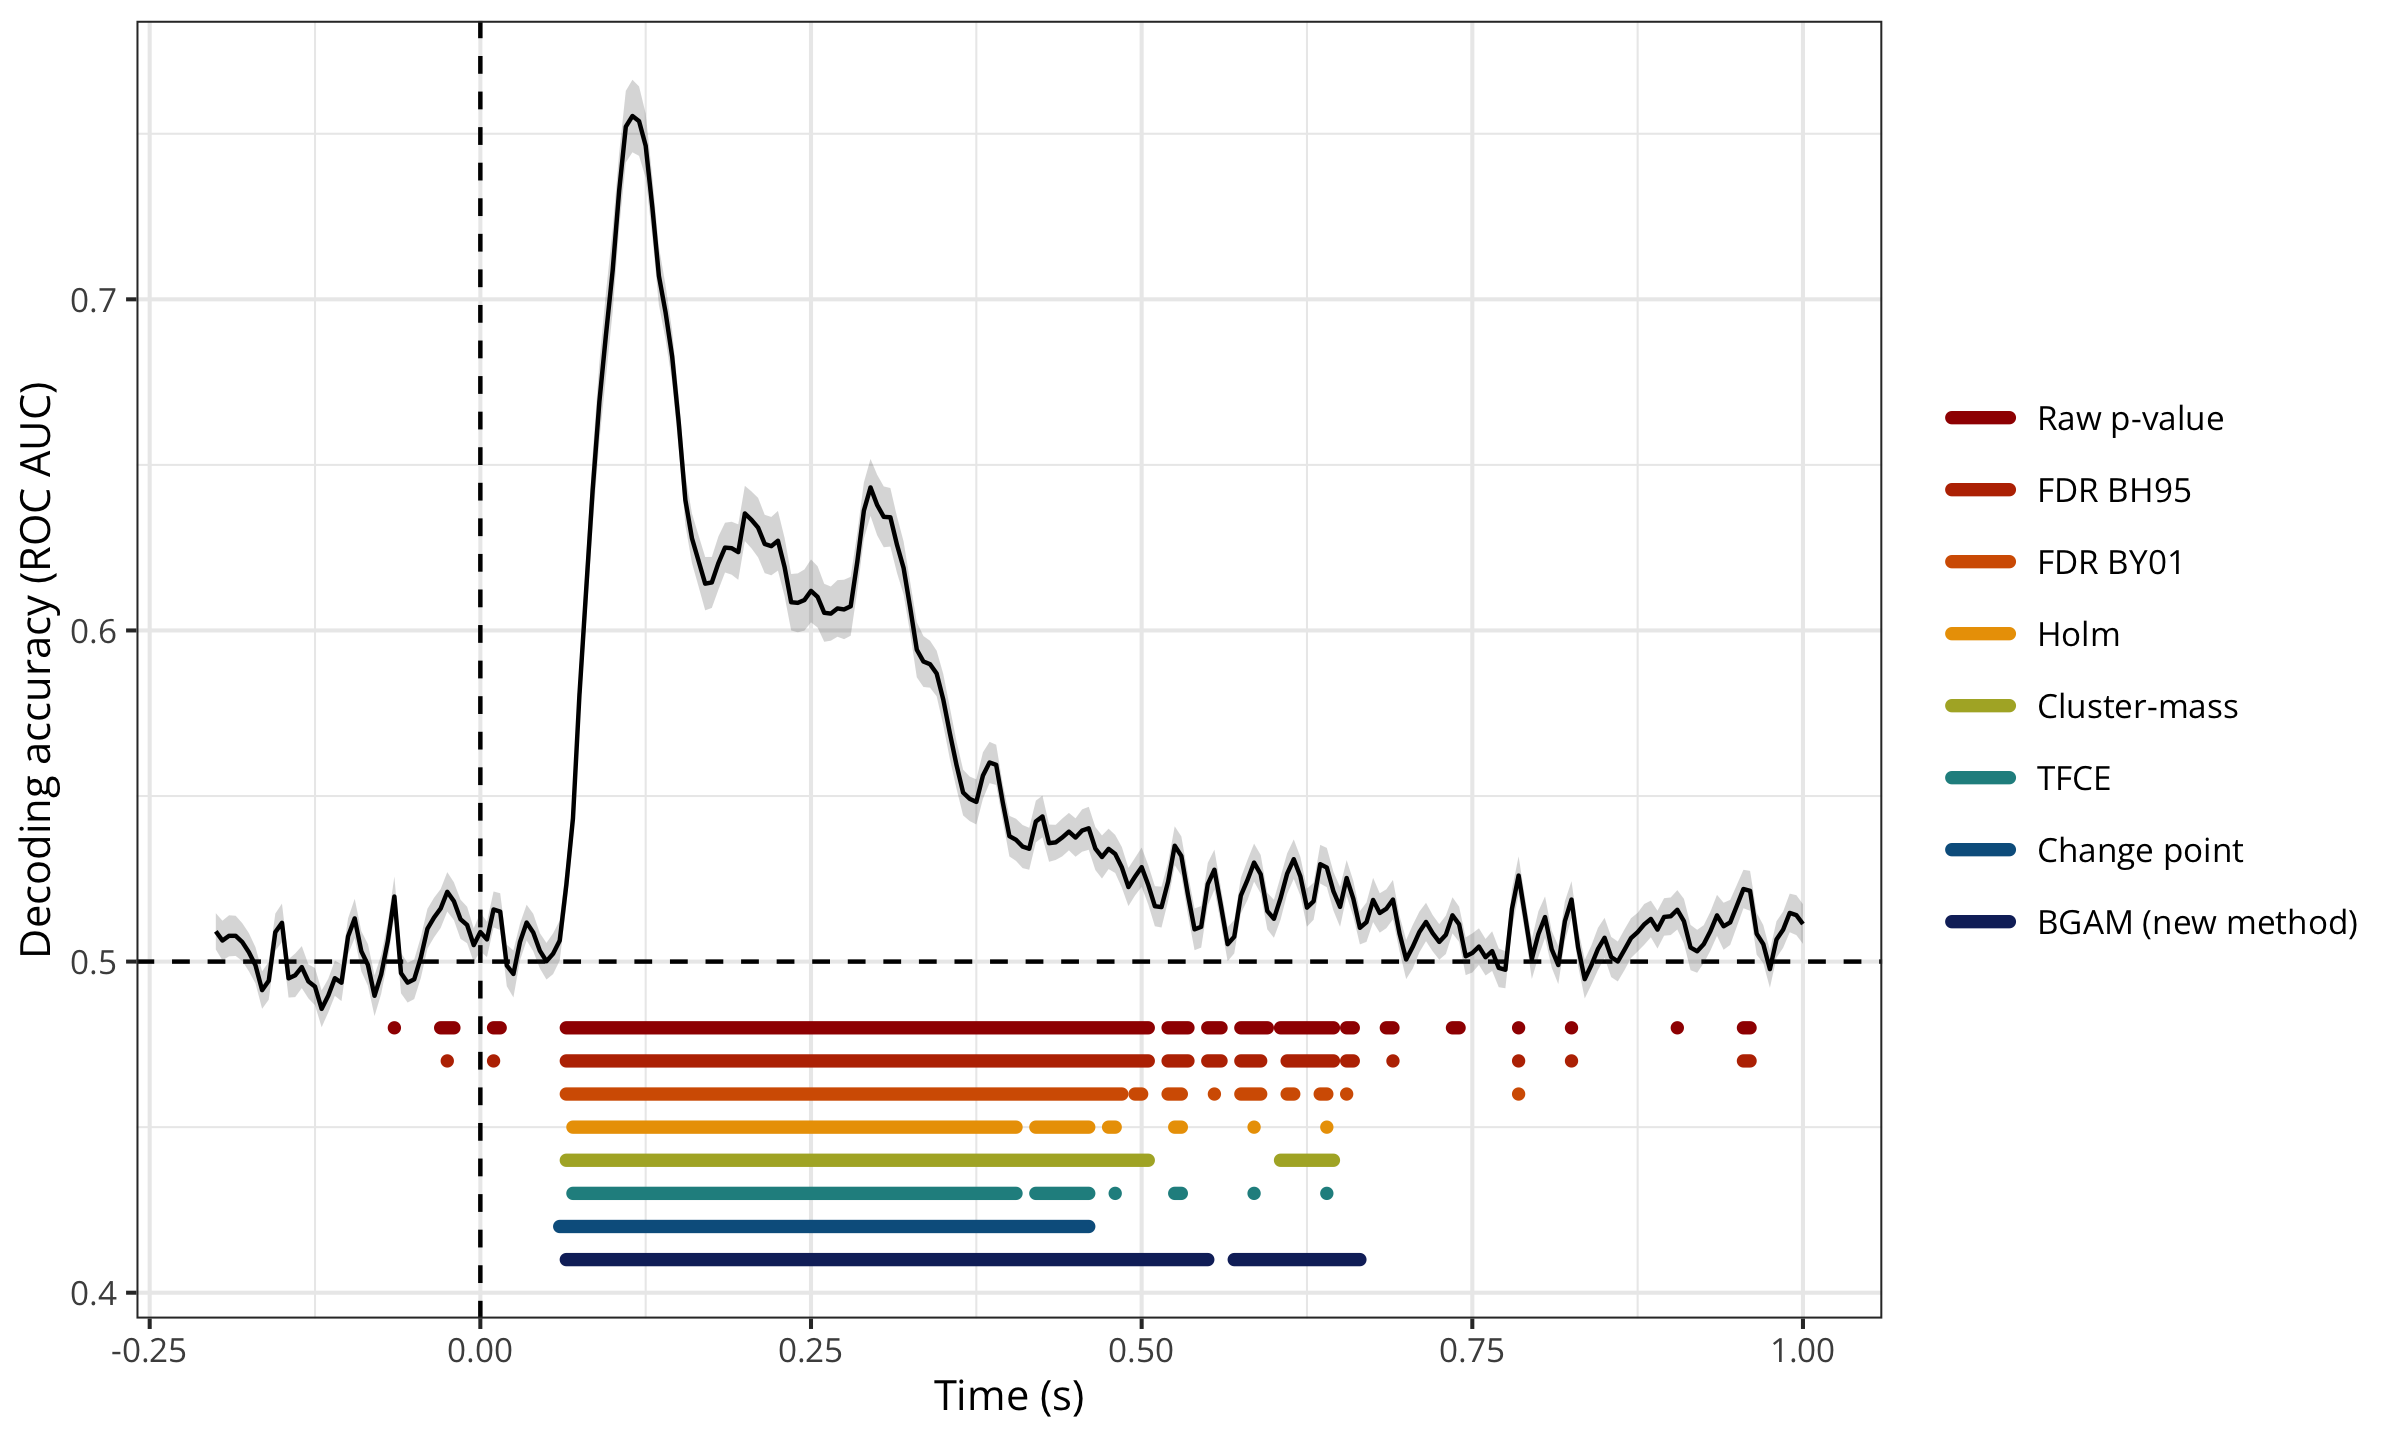
\includegraphics[width=1\textwidth,height=\textheight]{brms_meeg_files/figure-pdf/fig-onset-offset-1.png}

}

\end{figure}%

Figure~\ref{fig-reliability} shows the median difference between the
onset and offset estimates from each data split and the onset and offset
estimates from the full dataset (x-axis) along with the variance of its
onset and offset estimates across data splits (error bar). This figure
reveals that the \texttt{BGAM} \emph{onset and offset} estimates on each
split are the closest to the estimates from the full dataset on average
(0ms difference for the onset estimate and 5ms difference for the offset
estimate). The \texttt{Raw\ p-value} method has similar performance, but
given the aberrant estimates it produces (cf.
Figure~\ref{fig-onset-offset}), the fact that it is consistent between
data splits and the full dataset is not convincing on its own. The
\texttt{Change\ point} method also has a very good performance (i.e.,
very low difference between split estimates and full estimates), but
produces too short cluster of significant decoding performance (cf.
Figure~\ref{fig-onset-offset}).\footnote{As in Rousselet
  (\citeproc{ref-rousselet_using_2025}{2025}), we fixed the number of
  expected change points to two in the binary segmentation algorithm,
  thus producing always one cluster.} Overall, the figure reveals that
for all other methods, split datasets produce later onset estimates and
earlier offset estimates (as compared to the estimates from the model
fitted on the full dataset). These results highlight some desirable
properties for a method aiming to precisely and reliably estimate the
onset and offset of M/EEG effects, namely, it should i) have good
asymptotic properties on simulated data, ii) provide sensible identified
clusters in actual data, and iii) provide reliable/stable estimates on
actual data.

\begin{figure}[!htb]

\caption{\label{fig-reliability}Median error and median absolute
deviation of the error for the onset (left) and offset (right) estimates
according to each method. Methods are ordered from lowest (top) to
highest (bottom) median absolute error (separately for the onset and
offset estimates).}

\centering{

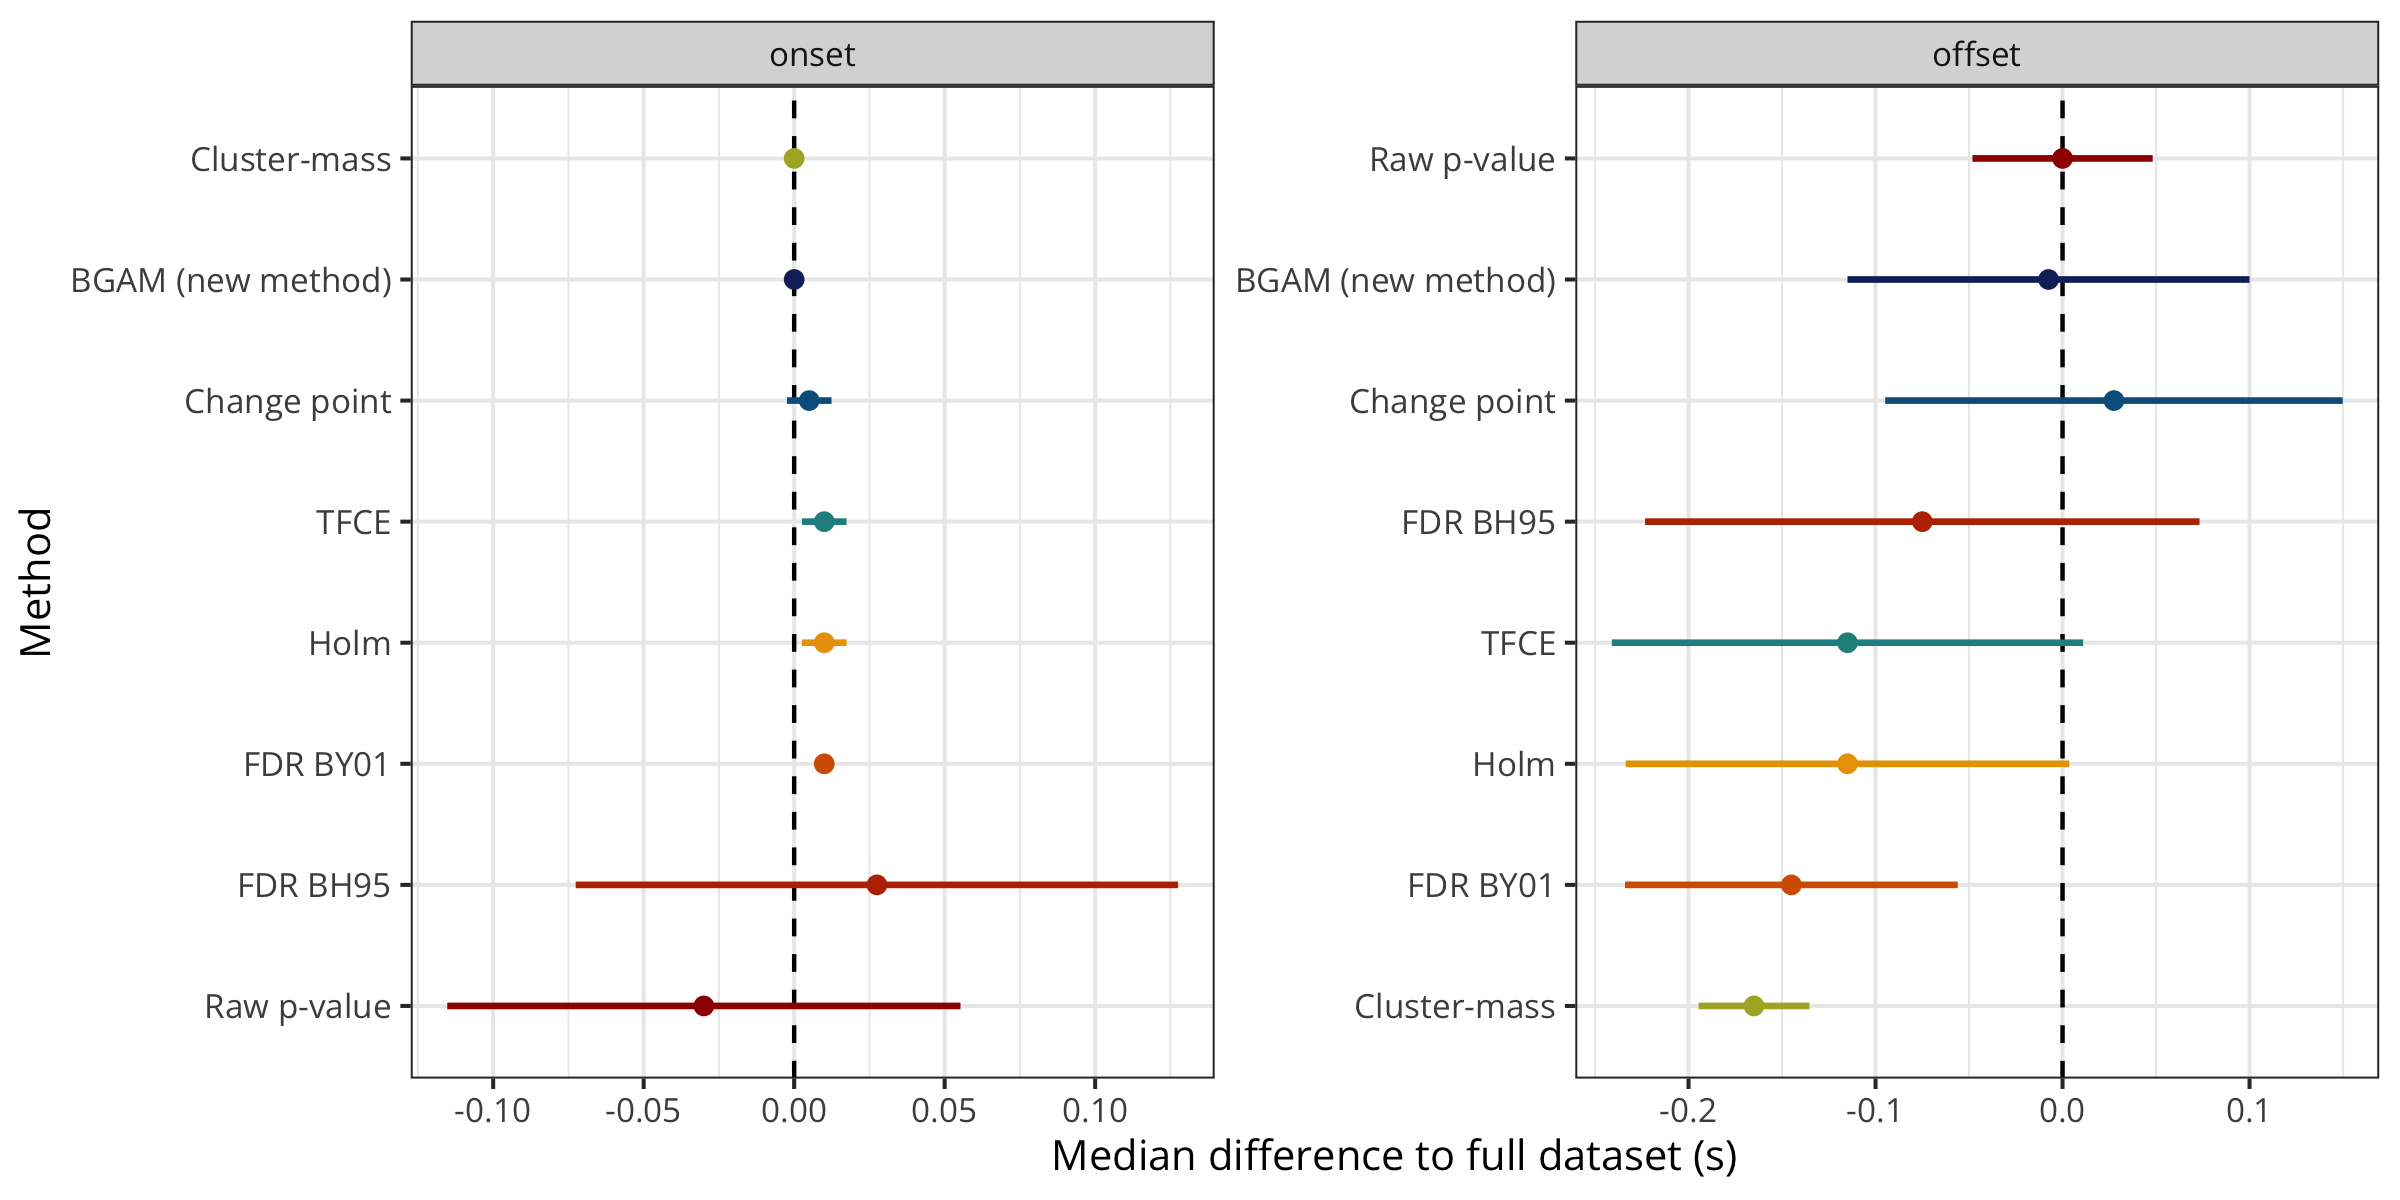
\includegraphics[width=1\textwidth,height=\textheight]{brms_meeg_files/figure-pdf/fig-reliability-1.png}

}

\end{figure}%

\begin{table}

{\caption{{Summary statistics of the onset and offset estimates for each
method (ordered by the absolute value of the
bias).}{\label{tbl-reliability-results}}}}

\fontsize{9.0pt}{10.8pt}\selectfont
\begin{tabular*}{\linewidth}{@{\extracolsep{\fill}}lccccc}
\toprule
 & Bias & MAE & RMSE & Variance & MAD \\ 
\midrule\addlinespace[2.5pt]
\multicolumn{6}{l}{onset} \\[2.5pt] 
\midrule\addlinespace[2.5pt]
BGAM (new method) & 0.0000 & 0.0000 & 0.0106 & 0.0008 & 0.0000 \\ 
Cluster mass & 0.0000 & 0.0000 & 0.0019 & 0.0000 & 0.0000 \\ 
Change point & 0.0050 & 0.0050 & 0.0011 & 0.0001 & 0.0074 \\ 
TFCE & 0.0100 & 0.0100 & 0.0120 & 0.0001 & 0.0074 \\ 
FDR BY01 & 0.0100 & 0.0100 & 0.0065 & 0.0023 & 0.0000 \\ 
Holm & 0.0100 & 0.0100 & 0.0118 & 0.0001 & 0.0074 \\ 
FDR BH95 & 0.0250 & 0.0900 & 0.0101 & 0.0076 & 0.0964 \\ 
Raw p-value & -0.0300 & 0.0650 & 0.0201 & 0.0062 & 0.0815 \\ 
\midrule\addlinespace[2.5pt]
\multicolumn{6}{l}{offset} \\[2.5pt] 
\midrule\addlinespace[2.5pt]
Raw p-value & 0.0000 & 0.0300 & 0.0256 & 0.0047 & 0.0445 \\ 
BGAM (new method) & -0.0050 & 0.0750 & 0.0716 & 0.0274 & 0.1038 \\ 
Change point & 0.0250 & 0.0650 & 0.0566 & 0.0090 & 0.1186 \\ 
FDR BH95 & -0.0750 & 0.0750 & 0.1053 & 0.0153 & 0.1483 \\ 
TFCE & -0.1150 & 0.1450 & 0.1094 & 0.0146 & 0.1260 \\ 
Holm & -0.1150 & 0.1450 & 0.1091 & 0.0133 & 0.1186 \\ 
FDR BY01 & -0.1450 & 0.1450 & 0.1197 & 0.0154 & 0.0890 \\ 
Cluster mass & -0.1650 & 0.1650 & 0.1448 & 0.0051 & 0.0297 \\ 
\bottomrule
\end{tabular*}

\end{table}

\newpage

\section{Discussion}\label{discussion}

\subsection{Summary of the proposed
approach}\label{summary-of-the-proposed-approach}

Overall, before concluding on the onset/offset of effect based on the
model, we need to ensure that the model provides a faithful description
of the data-generating process (e.g., via posterior predictive checks
etc)\ldots{}

The TFCE performs worse than the cluster-sum approach, which was
anticipated by Rousselet (\citeproc{ref-rousselet_using_2025}{2025})
based on the initial results of S. Smith \& Nichols
(\citeproc{ref-smith2009}{2009})\ldots{} we did not include the
cluster-depth algorithm (\citeproc{ref-frossard2022}{Frossard \& Renaud,
2022}), as Rousselet (\citeproc{ref-rousselet_using_2025}{2025}) already
showed its performance were worse than the cluster mass
algorithm\ldots{}

\subsection{Limitations and future
directions}\label{limitations-and-future-directions}

As in previous simulation work (e.g.,
\citeproc{ref-rousselet2008}{Rousselet et al., 2008};
\citeproc{ref-sassenhagen2019}{Sassenhagen \& Draschkow, 2019}), the
present simulation results depend on various choices such as the
specific cluster-forming algorithm and threshold, signal-to-noise ratio,
negative impact of preprocessing steps (e.g., low-pass filter) on
temporal resolution\ldots{} note however, that the same caveats apply to
all methods\ldots{}

Discussion about the nature of the model: we modelled the surface M/EEG
signals, however, the true interests (probably) lie in the brain, that
is, in the source space\ldots{} we could build a ``full'' Bayesian model
of the generated EEG signal (i.e., including hypotheses about the source
and a forward model), but this model would become computationally
heavier\ldots{}

The error properties depend on the threshold parameter, a value of 10 or
20 seems to be a reasonable default, but the optimal threshold parameter
can be adjusted using split-half reliability assessment\ldots{} also
depends on \texttt{k}\ldots{}

Can be applied to any 1D timeseries (e.g., pupillometry,
electromyography)\ldots{} Extending the approach to spatiotemporal data
(i.e., time + sensors) or spatiotemporal time-frequency 4D data\ldots{}

We kept the exemplary models simple, but can be extended by adding
varying/random effects (intercept and slope) for item (e.g.,
word)\ldots{} but also continuous predictors at the trial level?

\newpage

\section{Data and code availability}\label{data-and-code-availability}

The simulation results as well as the \texttt{R} code to reproduce the
simulations are available on GitHub:
\url{https://github.com/lnalborczyk/brms_meeg}. The \texttt{neurogam\ R}
package is available at \url{https://github.com/lnalborczyk/neurogam}.

\section{Packages}\label{packages}

We used R version 4.4.3 (\citeproc{ref-base}{R Core Team, 2025}) and the
following R packages: assertthat v. 0.2.1
(\citeproc{ref-assertthat}{Wickham, 2019}), brms v. 2.22.0
(\citeproc{ref-brms2017}{Bürkner, 2017}, \citeproc{ref-brms2018}{2018},
\citeproc{ref-brms2021}{2021}), changepoint v. 2.3
(\citeproc{ref-changepoint2024}{Killick et al., 2024};
\citeproc{ref-changepoint2014}{Killick \& Eckley, 2014}), doParallel v.
1.0.17 (\citeproc{ref-doParallel}{Corporation \& Weston, 2022}),
easystats v. 0.7.4 (\citeproc{ref-easystats}{Lüdecke et al., 2022}),
foreach v. 1.5.2 (\citeproc{ref-foreach}{Microsoft \& Weston, 2022}),
furrr v. 0.3.1 (\citeproc{ref-furrr}{Vaughan \& Dancho, 2022}), future
v. 1.34.0 (\citeproc{ref-RJ-2021-048}{Bengtsson, 2021}), ggrepel v.
0.9.6 (\citeproc{ref-ggrepel}{Slowikowski, 2024}), glue v. 1.8.0
(\citeproc{ref-glue}{Hester \& Bryan, 2024}), grateful v. 0.2.11
(\citeproc{ref-grateful}{Rodriguez-Sanchez \& Jackson, 2024}), gt v.
1.0.0 (\citeproc{ref-gt}{Iannone et al., 2025}), knitr v. 1.50
(\citeproc{ref-knitr2014}{Xie, 2014}, \citeproc{ref-knitr2015}{2015},
\citeproc{ref-knitr2025}{2025}), MetBrewer v. 0.2.0
(\citeproc{ref-MetBrewer}{Mills, 2022}), neurogam v. 0.0.1
(\citeproc{ref-neurogam}{Nalborczyk, 2025}), pakret v. 0.2.2
(\citeproc{ref-pakret}{Gallou, 2024}), patchwork v. 1.3.0
(\citeproc{ref-patchwork}{T. L. Pedersen, 2024}), rmarkdown v. 2.29
(\citeproc{ref-rmarkdown2024}{Allaire et al., 2024};
\citeproc{ref-rmarkdown2018}{Xie et al., 2018},
\citeproc{ref-rmarkdown2020}{2020}), scales v. 1.3.0
(\citeproc{ref-scales}{Wickham et al., 2023}), scico v. 1.5.0
(\citeproc{ref-scico}{T. L. Pedersen \& Crameri, 2023}), tictoc v. 1.2.1
(\citeproc{ref-tictoc}{Izrailev, 2024}), tidybayes v. 3.0.7
(\citeproc{ref-tidybayes}{Kay, 2024}), tidytext v. 0.4.2
(\citeproc{ref-tidytext}{Silge \& Robinson, 2016}), tidyverse v. 2.0.0
(\citeproc{ref-tidyverse}{Wickham et al., 2019}).

\section{Acknolwedgements}\label{acknolwedgements}

Centre de Calcul Intensif d'Aix-Marseille is acknowledged for granting
access to its high performance computing resources.

\newpage

\section{References}\label{references}

\phantomsection\label{refs}
\begin{CSLReferences}{1}{0}
\bibitem[\citeproctext]{ref-abugaber2023}
Abugaber, D., Finestrat, I., Luque, A., \& Morgan-Short, K. (2023).
Generalized additive mixed modeling of EEG supports dual-route accounts
of morphosyntax in suggesting no word frequency effects on processing of
regular grammatical forms. \emph{Journal of Neurolinguistics},
\emph{67}, 101137.
\url{https://doi.org/10.1016/j.jneuroling.2023.101137}

\bibitem[\citeproctext]{ref-rmarkdown2024}
Allaire, J., Xie, Y., Dervieux, C., McPherson, J., Luraschi, J., Ushey,
K., Atkins, A., Wickham, H., Cheng, J., Chang, W., \& Iannone, R.
(2024). \emph{{rmarkdown}: Dynamic documents for r}.
\url{https://github.com/rstudio/rmarkdown}

\bibitem[\citeproctext]{ref-baayen2020}
Baayen, R. H., \& Linke, M. (2020). \emph{Generalized Additive Mixed
Models} (pp. 563--591). Springer International Publishing.
\url{https://doi.org/10.1007/978-3-030-46216-1_23}

\bibitem[\citeproctext]{ref-baayen2018}
Baayen, R. H., Rij, J. van, Cat, C. de, \& Wood, S. (2018).
\emph{Autocorrelated errors in experimental data in the language
sciences: Some solutions offered by generalized additive mixed models}
(pp. 49--69). Springer International Publishing.
\url{https://doi.org/10.1007/978-3-319-69830-4_4}

\bibitem[\citeproctext]{ref-RJ-2021-048}
Bengtsson, H. (2021). A unifying framework for parallel and distributed
processing in r using futures. \emph{The R Journal}, \emph{13}(2),
208--227. \url{https://doi.org/10.32614/RJ-2021-048}

\bibitem[\citeproctext]{ref-benjamini1995}
Benjamini, Y., \& Hochberg, Y. (1995). Controlling the False Discovery
Rate: A Practical and Powerful Approach to Multiple Testing.
\emph{Journal of the Royal Statistical Society Series B: Statistical
Methodology}, \emph{57}(1), 289--300.
\url{https://doi.org/10.1111/j.2517-6161.1995.tb02031.x}

\bibitem[\citeproctext]{ref-benjamini2001}
Benjamini, Y., \& Yekutieli, D. (2001). The control of the false
discovery rate in multiple testing under dependency. \emph{The Annals of
Statistics}, \emph{29}(4). \url{https://doi.org/10.1214/aos/1013699998}

\bibitem[\citeproctext]{ref-bullmore1999}
Bullmore, E. T., Suckling, J., Overmeyer, S., Rabe-Hesketh, S., Taylor,
E., \& Brammer, M. J. (1999). Global, voxel, and cluster tests, by
theory and permutation, for a difference between two groups of
structural MR images of the brain. \emph{IEEE Transactions on Medical
Imaging}, \emph{18}(1), 32--42. \url{https://doi.org/10.1109/42.750253}

\bibitem[\citeproctext]{ref-brms2017}
Bürkner, P.-C. (2017). {brms}: An {R} package for {Bayesian} multilevel
models using {Stan}. \emph{Journal of Statistical Software},
\emph{80}(1), 1--28. \url{https://doi.org/10.18637/jss.v080.i01}

\bibitem[\citeproctext]{ref-brms2018}
Bürkner, P.-C. (2018). Advanced {Bayesian} multilevel modeling with the
{R} package {brms}. \emph{The R Journal}, \emph{10}(1), 395--411.
\url{https://doi.org/10.32614/RJ-2018-017}

\bibitem[\citeproctext]{ref-brms2021}
Bürkner, P.-C. (2021). Bayesian item response modeling in {R} with
{brms} and {Stan}. \emph{Journal of Statistical Software},
\emph{100}(5), 1--54. \url{https://doi.org/10.18637/jss.v100.i05}

\bibitem[\citeproctext]{ref-coretta2025}
Coretta, S., \& Bürkner, P.-. C. (2025). \emph{Bayesian beta regressions
with brms in r: A tutorial for phoneticians}.
\url{http://dx.doi.org/10.31219/osf.io/f9rqg_v1}

\bibitem[\citeproctext]{ref-doParallel}
Corporation, M., \& Weston, S. (2022). \emph{{doParallel}: Foreach
parallel adaptor for the {``{parallel}''} package}.
\url{https://CRAN.R-project.org/package=doParallel}

\bibitem[\citeproctext]{ref-delorme2004}
Delorme, A., \& Makeig, S. (2004). EEGLAB: an open source toolbox for
analysis of single-trial EEG dynamics including independent component
analysis. \emph{Journal of Neuroscience Methods}, \emph{134}(1), 9--21.
\url{https://doi.org/10.1016/j.jneumeth.2003.10.009}

\bibitem[\citeproctext]{ref-dimigen2021}
Dimigen, O., \& Ehinger, B. V. (2021). Regression-based analysis of
combined EEG and eye-tracking data: Theory and applications.
\emph{Journal of Vision}, \emph{21}(1), 3.
\url{https://doi.org/10.1167/jov.21.1.3}

\bibitem[\citeproctext]{ref-dinga2021}
Dinga, R., Fraza, C. J., Bayer, J. M. M., Kia, S. M., Beckmann, C. F.,
\& Marquand, A. F. (2021). \emph{Normative modeling of neuroimaging data
using generalized additive models of location scale and shape}.
\url{http://dx.doi.org/10.1101/2021.06.14.448106}

\bibitem[\citeproctext]{ref-dunagan2024}
Dunagan, D., Jordan, T., Hale, J. T., Pylkkänen, L., \& Chacón, D. A.
(2024). \emph{Evaluating the timecourses of morpho-orthographic,
lexical, and grammatical processing following rapid parallel visual
presentation: An EEG investigation in english}.
\url{http://dx.doi.org/10.1101/2024.04.10.588861}

\bibitem[\citeproctext]{ref-dunn1961}
Dunn, O. J. (1961). Multiple Comparisons among Means. \emph{Journal of
the American Statistical Association}, \emph{56}(293), 52--64.
\url{https://doi.org/10.1080/01621459.1961.10482090}

\bibitem[\citeproctext]{ref-ehinger_unfold_2019}
Ehinger, B. V., \& Dimigen, O. (2019). Unfold: An integrated toolbox for
overlap correction, non-linear modeling, and regression-based {EEG}
analysis. \emph{PeerJ}, \emph{7}, e7838.
\url{https://doi.org/10.7717/peerj.7838}

\bibitem[\citeproctext]{ref-fischer2013}
Fischer, Adrian~G., \& Ullsperger, M. (2013). Real and Fictive Outcomes
Are Processed Differently but Converge on a Common Adaptive Mechanism.
\emph{Neuron}, \emph{79}(6), 1243--1255.
\url{https://doi.org/10.1016/j.neuron.2013.07.006}

\bibitem[\citeproctext]{ref-frossard2022}
Frossard, J., \& Renaud, O. (2022). The cluster depth tests: Toward
point-wise strong control of the family-wise error rate in massively
univariate tests with application to M/EEG. \emph{NeuroImage},
\emph{247}, 118824.
\url{https://doi.org/10.1016/j.neuroimage.2021.118824}

\bibitem[\citeproctext]{ref-gabry2019}
Gabry, J., Simpson, D., Vehtari, A., Betancourt, M., \& Gelman, A.
(2019). Visualization in Bayesian work{fl}ow. \emph{Journal of the Royal
Statistical Society: Series A (Statistics in Society)}, \emph{182}(2),
389--402. \url{https://doi.org/10.1111/rssa.12378}

\bibitem[\citeproctext]{ref-pakret}
Gallou, A. (2024). \emph{{pakret}: Cite {``{R}''} packages on the fly in
{``{R Markdown}''} and {``{Quarto}''}}.
\url{https://CRAN.R-project.org/package=pakret}

\bibitem[\citeproctext]{ref-gelman2020}
Gelman, A., Vehtari, A., Simpson, D., Margossian, C. C., Carpenter, B.,
Yao, Y., Kennedy, L., Gabry, J., Bürkner, P.-C., \& Modrák, M. (2020).
Bayesian workflow. \emph{arXiv:2011.01808 {[}Stat{]}}.
\url{http://arxiv.org/abs/2011.01808}

\bibitem[\citeproctext]{ref-gramfort2013}
Gramfort, A. (2013). MEG and EEG data analysis with MNE-python.
\emph{Frontiers in Neuroscience}, \emph{7}.
\url{https://doi.org/10.3389/fnins.2013.00267}

\bibitem[\citeproctext]{ref-hastie2017}
Hastie, T. J., \& Tibshirani, R. J. (2017). \emph{Generalized Additive
Models}. Routledge. \url{https://doi.org/10.1201/9780203753781}

\bibitem[\citeproctext]{ref-hauk2006}
Hauk, O., Davis, M. H., Ford, M., Pulvermüller, F., \& Marslen-Wilson,
W. D. (2006). The time course of visual word recognition as revealed by
linear regression analysis of ERP data. \emph{NeuroImage}, \emph{30}(4),
1383--1400. \url{https://doi.org/10.1016/j.neuroimage.2005.11.048}

\bibitem[\citeproctext]{ref-hendrix2017}
Hendrix, P., Bolger, P., \& Baayen, H. (2017). Distinct ERP signatures
of word frequency, phrase frequency, and prototypicality in speech
production. \emph{Journal of Experimental Psychology: Learning, Memory,
and Cognition}, \emph{43}(1), 128--149.
\url{https://doi.org/10.1037/a0040332}

\bibitem[\citeproctext]{ref-glue}
Hester, J., \& Bryan, J. (2024). \emph{{glue}: Interpreted string
literals}. \url{https://CRAN.R-project.org/package=glue}

\bibitem[\citeproctext]{ref-holm1979}
Holm, S. (1979). A simple sequentially rejective multiple test
procedure. \emph{Scandinavian Journal of Statistics}, \emph{6}(2),
65--70. \url{http://www.jstor.org/stable/4615733}

\bibitem[\citeproctext]{ref-gt}
Iannone, R., Cheng, J., Schloerke, B., Hughes, E., Lauer, A., Seo, J.,
Brevoort, K., \& Roy, O. (2025). \emph{{gt}: Easily create
presentation-ready display tables}.
\url{https://CRAN.R-project.org/package=gt}

\bibitem[\citeproctext]{ref-tictoc}
Izrailev, S. (2024). \emph{{tictoc}: Functions for timing r scripts, as
well as implementations of {``{Stack}''} and {``{StackList}''}
structures}. \url{https://CRAN.R-project.org/package=tictoc}

\bibitem[\citeproctext]{ref-tidybayes}
Kay, M. (2024). \emph{{tidybayes}: Tidy data and geoms for {Bayesian}
models}. \url{https://doi.org/10.5281/zenodo.1308151}

\bibitem[\citeproctext]{ref-changepoint2014}
Killick, R., \& Eckley, I. A. (2014). {changepoint}: An {R} package for
changepoint analysis. \emph{Journal of Statistical Software},
\emph{58}(3), 1--19.
\url{https://www.jstatsoft.org/article/view/v058i03}

\bibitem[\citeproctext]{ref-changepoint}
Killick, R., Haynes, K., \& Eckley, I. A. (2022). \emph{{changepoint}:
An {R} package for changepoint analysis}.
\url{https://CRAN.R-project.org/package=changepoint}

\bibitem[\citeproctext]{ref-changepoint2024}
Killick, R., Haynes, K., \& Eckley, I. A. (2024). \emph{{changepoint}:
An {R} package for changepoint analysis}.
\url{https://CRAN.R-project.org/package=changepoint}

\bibitem[\citeproctext]{ref-king2014}
King, J.-R., \& Dehaene, S. (2014). Characterizing the dynamics of
mental representations: the temporal generalization method. \emph{Trends
in Cognitive Sciences}, \emph{18}(4), 203--210.
\url{https://doi.org/10.1016/j.tics.2014.01.002}

\bibitem[\citeproctext]{ref-kruschke2017}
Kruschke, J. K., \& Liddell, T. M. (2017). The Bayesian New Statistics:
Hypothesis testing, estimation, meta-analysis, and power analysis from a
Bayesian perspective. \emph{Psychonomic Bulletin \& Review},
\emph{25}(1), 178--206. \url{https://doi.org/10.3758/s13423-016-1221-4}

\bibitem[\citeproctext]{ref-kryuchkova2012}
Kryuchkova, T., Tucker, B. V., Wurm, L. H., \& Baayen, R. H. (2012).
Danger and usefulness are detected early in auditory lexical processing:
Evidence from electroencephalography. \emph{Brain and Language},
\emph{122}(2), 81--91. \url{https://doi.org/10.1016/j.bandl.2012.05.005}

\bibitem[\citeproctext]{ref-easystats}
Lüdecke, D., Ben-Shachar, M. S., Patil, I., Wiernik, B. M., Bacher, E.,
Thériault, R., \& Makowski, D. (2022). {easystats}: Framework for easy
statistical modeling, visualization, and reporting. \emph{CRAN}.
\url{https://doi.org/10.32614/CRAN.package.easystats}

\bibitem[\citeproctext]{ref-maris2011}
Maris, E. (2011). Statistical testing in electrophysiological studies.
\emph{Psychophysiology}, \emph{49}(4), 549--565.
\url{https://doi.org/10.1111/j.1469-8986.2011.01320.x}

\bibitem[\citeproctext]{ref-maris2007}
Maris, E., \& Oostenveld, R. (2007). Nonparametric statistical testing
of EEG- and MEG-data. \emph{Journal of Neuroscience Methods},
\emph{164}(1), 177--190.
\url{https://doi.org/10.1016/j.jneumeth.2007.03.024}

\bibitem[\citeproctext]{ref-meulman2023}
Meulman, N., Sprenger, S. A., Schmid, M. S., \& Wieling, M. (2023).
GAM-based individual difference measures for L2 ERP studies.
\emph{Research Methods in Applied Linguistics}, \emph{2}(3), 100079.
\url{https://doi.org/10.1016/j.rmal.2023.100079}

\bibitem[\citeproctext]{ref-meulman2015}
Meulman, N., Wieling, M., Sprenger, S. A., Stowe, L. A., \& Schmid, M.
S. (2015). Age Effects in L2 Grammar Processing as Revealed by ERPs and
How (Not) to Study Them. \emph{PLOS ONE}, \emph{10}(12), e0143328.
\url{https://doi.org/10.1371/journal.pone.0143328}

\bibitem[\citeproctext]{ref-foreach}
Microsoft, \& Weston, S. (2022). \emph{{foreach}: Provides foreach
looping construct}. \url{https://CRAN.R-project.org/package=foreach}

\bibitem[\citeproctext]{ref-miller2025}
Miller, D. L. (2025). Bayesian views of generalized additive modelling.
\emph{Methods in Ecology and Evolution}.
\url{https://doi.org/10.1111/2041-210x.14498}

\bibitem[\citeproctext]{ref-MetBrewer}
Mills, B. R. (2022). \emph{{MetBrewer}: Color palettes inspired by works
at the metropolitan museum of art}.
\url{https://CRAN.R-project.org/package=MetBrewer}

\bibitem[\citeproctext]{ref-neurogam}
Nalborczyk, L. (2025). \emph{{neurogam}: Precise temporal localisation
of m/EEG effects with bayesian generalised additive multilevel models}.
\url{https://github.com/lnalborczyk/neurogam}

\bibitem[\citeproctext]{ref-nalborczyk2019}
Nalborczyk, L., Batailler, C., Lœvenbruck, H., Vilain, A., \& Bürkner,
P.-C. (2019). An Introduction to Bayesian Multilevel Models Using brms:
A Case Study of Gender Effects on Vowel Variability in Standard
Indonesian. \emph{Journal of Speech, Language, and Hearing Research},
\emph{62}(5), 1225--1242.
\url{https://doi.org/10.1044/2018_jslhr-s-18-0006}

\bibitem[\citeproctext]{ref-nalborczyk:inprep}
Nalborczyk, L., Hauw, F., Torcy, H. de, Dehaene, S., \& Cohen, L. (in
preparation). \emph{Neural and representational dynamics of tickertape
synesthesia}.

\bibitem[\citeproctext]{ref-pedersen_hierarchical_2019}
Pedersen, E. J., Miller, D. L., Simpson, G. L., \& Ross, N. (2019).
Hierarchical generalized additive models in ecology: An introduction
with mgcv. \emph{PeerJ}, \emph{7}, e6876.
\url{https://doi.org/10.7717/peerj.6876}

\bibitem[\citeproctext]{ref-patchwork}
Pedersen, T. L. (2024). \emph{{patchwork}: The composer of plots}.
\url{https://CRAN.R-project.org/package=patchwork}

\bibitem[\citeproctext]{ref-scico}
Pedersen, T. L., \& Crameri, F. (2023). \emph{{scico}: Colour palettes
based on the scientific colour-maps}.
\url{https://CRAN.R-project.org/package=scico}

\bibitem[\citeproctext]{ref-pernet2022}
Pernet, C. R. (2022). Electroencephalography robust statistical linear
modelling using a single weight per trial. \emph{Aperture Neuro},
\emph{2}, 1--22.
\url{https://doi.org/10.52294/apertureneuro.2022.2.seoo9435}

\bibitem[\citeproctext]{ref-pernet2011}
Pernet, C. R., Chauveau, N., Gaspar, C., \& Rousselet, G. A. (2011).
LIMO EEG: A Toolbox for Hierarchical LInear MOdeling of
ElectroEncephaloGraphic Data. \emph{Computational Intelligence and
Neuroscience}, \emph{2011}, 1--11.
\url{https://doi.org/10.1155/2011/831409}

\bibitem[\citeproctext]{ref-pernet2015}
Pernet, C. R., Latinus, M., Nichols, T. E., \& Rousselet, G. A. (2015).
Cluster-based computational methods for mass univariate analyses of
event-related brain potentials/fields: A simulation study. \emph{Journal
of Neuroscience Methods}, \emph{250}, 85--93.
\url{https://doi.org/10.1016/j.jneumeth.2014.08.003}

\bibitem[\citeproctext]{ref-base}
R Core Team. (2025). \emph{{R}: A language and environment for
statistical computing}. R Foundation for Statistical Computing.
\url{https://www.R-project.org/}

\bibitem[\citeproctext]{ref-rasmussen2005}
Rasmussen, C. E., \& Williams, C. K. I. (2005). \emph{Gaussian Processes
for Machine Learning}.
\url{https://doi.org/10.7551/mitpress/3206.001.0001}

\bibitem[\citeproctext]{ref-rigby2005}
Rigby, R. A., \& Stasinopoulos, D. M. (2005). Generalized Additive
Models for Location, Scale and Shape. \emph{Journal of the Royal
Statistical Society Series C: Applied Statistics}, \emph{54}(3),
507--554. \url{https://doi.org/10.1111/j.1467-9876.2005.00510.x}

\bibitem[\citeproctext]{ref-vanrij2019}
Rij, J. van, Hendriks, P., Rijn, H. van, Baayen, R. H., \& Wood, S. N.
(2019). Analyzing the Time Course of Pupillometric Data. \emph{Trends in
Hearing}, \emph{23}. \url{https://doi.org/10.1177/2331216519832483}

\bibitem[\citeproctext]{ref-riutort-mayol_practical_2023}
Riutort-Mayol, G., Bürkner, P.-C., Andersen, M. R., Solin, A., \&
Vehtari, A. (2023). Practical {Hilbert} space approximate {Bayesian
Gaussian} processes for probabilistic programming. \emph{Statistics and
Computing}, \emph{33}(1), 17.
\url{https://doi.org/10.1007/s11222-022-10167-2}

\bibitem[\citeproctext]{ref-grateful}
Rodriguez-Sanchez, F., \& Jackson, C. P. (2024). \emph{{grateful}:
Facilitate citation of {R} packages}.
\url{https://pakillo.github.io/grateful/}

\bibitem[\citeproctext]{ref-rosenblatt2018}
Rosenblatt, J. D., Finos, L., Weeda, W. D., Solari, A., \& Goeman, J. J.
(2018). All-Resolutions Inference for brain imaging. \emph{NeuroImage},
\emph{181}, 786--796.
\url{https://doi.org/10.1016/j.neuroimage.2018.07.060}

\bibitem[\citeproctext]{ref-rousselet_using_2025}
Rousselet, G. A. (2025). Using cluster-based permutation tests to
estimate {MEG}/{EEG} onsets: {How} bad is it? \emph{European Journal of
Neuroscience}, \emph{61}(1), e16618.
\url{https://doi.org/10.1111/ejn.16618}

\bibitem[\citeproctext]{ref-rousselet2008}
Rousselet, G. A., Pernet, C. R., Bennett, P. J., \& Sekuler, A. B.
(2008). Parametric study of EEG sensitivity to phase noise during face
processing. \emph{BMC Neuroscience}, \emph{9}(1).
\url{https://doi.org/10.1186/1471-2202-9-98}

\bibitem[\citeproctext]{ref-sassenhagen2019}
Sassenhagen, J., \& Draschkow, D. (2019). Cluster{-}based permutation
tests of MEG/EEG data do not establish significance of effect latency or
location. \emph{Psychophysiology}, \emph{56}(6).
\url{https://doi.org/10.1111/psyp.13335}

\bibitem[\citeproctext]{ref-tidytext}
Silge, J., \& Robinson, D. (2016). {tidytext}: Text mining and analysis
using tidy data principles in r. \emph{JOSS}, \emph{1}(3).
\url{https://doi.org/10.21105/joss.00037}

\bibitem[\citeproctext]{ref-skukies_modelling_2021}
Skukies, R., \& Ehinger, B. (2021). Modelling event duration and overlap
during {EEG} analysis. \emph{Journal of Vision}, \emph{21}(9), 2037.
\url{https://doi.org/10.1167/jov.21.9.2037}

\bibitem[\citeproctext]{ref-skukies_brain_2024}
Skukies, R., Schepers, J., \& Ehinger, B. (2024, December 9).
\emph{Brain responses vary in duration - modeling strategies and
challenges}. \url{https://doi.org/10.1101/2024.12.05.626938}

\bibitem[\citeproctext]{ref-ggrepel}
Slowikowski, K. (2024). \emph{{ggrepel}: Automatically position
non-overlapping text labels with {``{ggplot2}''}}.
\url{https://CRAN.R-project.org/package=ggrepel}

\bibitem[\citeproctext]{ref-smith2014a}
Smith, N. J., \& Kutas, M. (2014a). Regression{-}based estimation of ERP
waveforms: I. The rERP framework. \emph{Psychophysiology}, \emph{52}(2),
157--168. \url{https://doi.org/10.1111/psyp.12317}

\bibitem[\citeproctext]{ref-smith2014b}
Smith, N. J., \& Kutas, M. (2014b). Regression{-}based estimation of ERP
waveforms: II. Nonlinear effects, overlap correction, and practical
considerations. \emph{Psychophysiology}, \emph{52}(2), 169--181.
\url{https://doi.org/10.1111/psyp.12320}

\bibitem[\citeproctext]{ref-smith2009}
Smith, S., \& Nichols, T. (2009). Threshold-free cluster enhancement:
Addressing problems of smoothing, threshold dependence and localisation
in cluster inference. \emph{NeuroImage}, \emph{44}(1), 83--98.
\url{https://doi.org/10.1016/j.neuroimage.2008.03.061}

\bibitem[\citeproctext]{ref-suxf3skuthy2017}
Sóskuthy, M. (2017). \emph{Generalised additive mixed models for dynamic
analysis in linguistics: A practical introduction}.
\url{https://doi.org/10.48550/ARXIV.1703.05339}

\bibitem[\citeproctext]{ref-suxf3skuthy2021}
Sóskuthy, M. (2021). Evaluating generalised additive mixed modelling
strategies for dynamic speech analysis. \emph{Journal of Phonetics},
\emph{84}, 101017. \url{https://doi.org/10.1016/j.wocn.2020.101017}

\bibitem[\citeproctext]{ref-teichmann2022}
Teichmann, L. (2022). An empirically driven guide on using bayes factors
for m/EEG decoding. \emph{Aperture Neuro}, \emph{2}, 1--10.
\url{https://doi.org/10.52294/apertureneuro.2022.2.maoc6465}

\bibitem[\citeproctext]{ref-tremblay2014}
Tremblay, A., \& Newman, A. J. (2014). Modeling nonlinear relationships
in ERP data using mixed{-}effects regression with R examples.
\emph{Psychophysiology}, \emph{52}(1), 124--139.
\url{https://doi.org/10.1111/psyp.12299}

\bibitem[\citeproctext]{ref-umlauf2018}
Umlauf, N., Klein, N., \& Zeileis, A. (2018). BAMLSS: Bayesian Additive
Models for Location, Scale, and Shape (and Beyond). \emph{Journal of
Computational and Graphical Statistics}, \emph{27}(3), 612--627.
\url{https://doi.org/10.1080/10618600.2017.1407325}

\bibitem[\citeproctext]{ref-reticulate}
Ushey, K., Allaire, J., \& Tang, Y. (2024). \emph{Reticulate: Interface
to 'python'}. \url{https://CRAN.R-project.org/package=reticulate}

\bibitem[\citeproctext]{ref-furrr}
Vaughan, D., \& Dancho, M. (2022). \emph{{furrr}: Apply mapping
functions in parallel using futures}.
\url{https://CRAN.R-project.org/package=furrr}

\bibitem[\citeproctext]{ref-assertthat}
Wickham, H. (2019). \emph{{assertthat}: Easy pre and post assertions}.
\url{https://CRAN.R-project.org/package=assertthat}

\bibitem[\citeproctext]{ref-tidyverse}
Wickham, H., Averick, M., Bryan, J., Chang, W., McGowan, L. D.,
François, R., Grolemund, G., Hayes, A., Henry, L., Hester, J., Kuhn, M.,
Pedersen, T. L., Miller, E., Bache, S. M., Müller, K., Ooms, J.,
Robinson, D., Seidel, D. P., Spinu, V., \ldots{} Yutani, H. (2019).
Welcome to the {tidyverse}. \emph{Journal of Open Source Software},
\emph{4}(43), 1686. \url{https://doi.org/10.21105/joss.01686}

\bibitem[\citeproctext]{ref-scales}
Wickham, H., Pedersen, T. L., \& Seidel, D. (2023). \emph{{scales}:
Scale functions for visualization}.
\url{https://CRAN.R-project.org/package=scales}

\bibitem[\citeproctext]{ref-wieling2018}
Wieling, M. (2018). Analyzing dynamic phonetic data using generalized
additive mixed modeling: A tutorial focusing on articulatory differences
between L1 and L2 speakers of English. \emph{Journal of Phonetics},
\emph{70}, 86--116. \url{https://doi.org/10.1016/j.wocn.2018.03.002}

\bibitem[\citeproctext]{ref-winter2016}
Winter, B., \& Wieling, M. (2016). How to analyze linguistic change
using mixed models, Growth Curve Analysis and Generalized Additive
Modeling. \emph{Journal of Language Evolution}, \emph{1}(1), 7--18.
\url{https://doi.org/10.1093/jole/lzv003}

\bibitem[\citeproctext]{ref-wood2003}
Wood, S. N. (2003). Thin Plate Regression Splines. \emph{Journal of the
Royal Statistical Society Series B: Statistical Methodology},
\emph{65}(1), 95--114. \url{https://doi.org/10.1111/1467-9868.00374}

\bibitem[\citeproctext]{ref-wood2017}
Wood, S. N. (2017a). \emph{Generalized Additive Models}. Chapman;
Hall/CRC. \url{https://doi.org/10.1201/9781315370279}

\bibitem[\citeproctext]{ref-mgcv}
Wood, S. N. (2017b). \emph{Generalized additive models: An introduction
with r} (2nd ed.). Chapman; Hall/CRC.

\bibitem[\citeproctext]{ref-wuxfcllhorst2025}
Wüllhorst, V., Wüllhorst, R., Overmeyer, R., \& Endrass, T. (2025).
Comprehensive Analysis of Event{-}Related Potentials of Response
Inhibition: The Role of Negative Urgency and Compulsivity.
\emph{Psychophysiology}, \emph{62}(2).
\url{https://doi.org/10.1111/psyp.70000}

\bibitem[\citeproctext]{ref-knitr2014}
Xie, Y. (2014). {knitr}: A comprehensive tool for reproducible research
in {R}. In V. Stodden, F. Leisch, \& R. D. Peng (Eds.),
\emph{Implementing reproducible computational research}. Chapman;
Hall/CRC.

\bibitem[\citeproctext]{ref-knitr2015}
Xie, Y. (2015). \emph{Dynamic documents with {R} and knitr} (2nd ed.).
Chapman; Hall/CRC. \url{https://yihui.org/knitr/}

\bibitem[\citeproctext]{ref-knitr2025}
Xie, Y. (2025). \emph{{knitr}: A general-purpose package for dynamic
report generation in {R}}. \url{https://yihui.org/knitr/}

\bibitem[\citeproctext]{ref-rmarkdown2018}
Xie, Y., Allaire, J. J., \& Grolemund, G. (2018). \emph{R markdown: The
definitive guide}. Chapman; Hall/CRC.
\url{https://bookdown.org/yihui/rmarkdown}

\bibitem[\citeproctext]{ref-rmarkdown2020}
Xie, Y., Dervieux, C., \& Riederer, E. (2020). \emph{R markdown
cookbook}. Chapman; Hall/CRC.
\url{https://bookdown.org/yihui/rmarkdown-cookbook}

\bibitem[\citeproctext]{ref-yeung2004}
Yeung, N., Bogacz, R., Holroyd, C. B., \& Cohen, J. D. (2004). Detection
of synchronized oscillations in the electroencephalogram: An evaluation
of methods. \emph{Psychophysiology}, \emph{41}(6), 822--832.
\url{https://doi.org/10.1111/j.1469-8986.2004.00239.x}

\end{CSLReferences}

\newpage

\appendix

\section{Application to 2D time-resolved decoding results
(cross-temporal generalisation)}\label{sec-2D}

Assume we have M/EEG data and we have conducted cross-temporal
generalisation analyses (\citeproc{ref-king2014}{King \& Dehaene,
2014}). As a result, we have a 2D matrix where each element contains the
decoding accuracy (e.g., ROC AUC) of a classifier trained at timestep
\(\text{training}_{i}\) and tested at timestep \(\text{testing}_{j}\)
(Figure~\ref{fig-sim-timegen}).

\begin{figure}[!htb]

\caption{\label{fig-sim-timegen}Exemplary (simulated) group-level
average cross-temporal generalisation matrix of decoding performance
(ROC AUC).}

\centering{

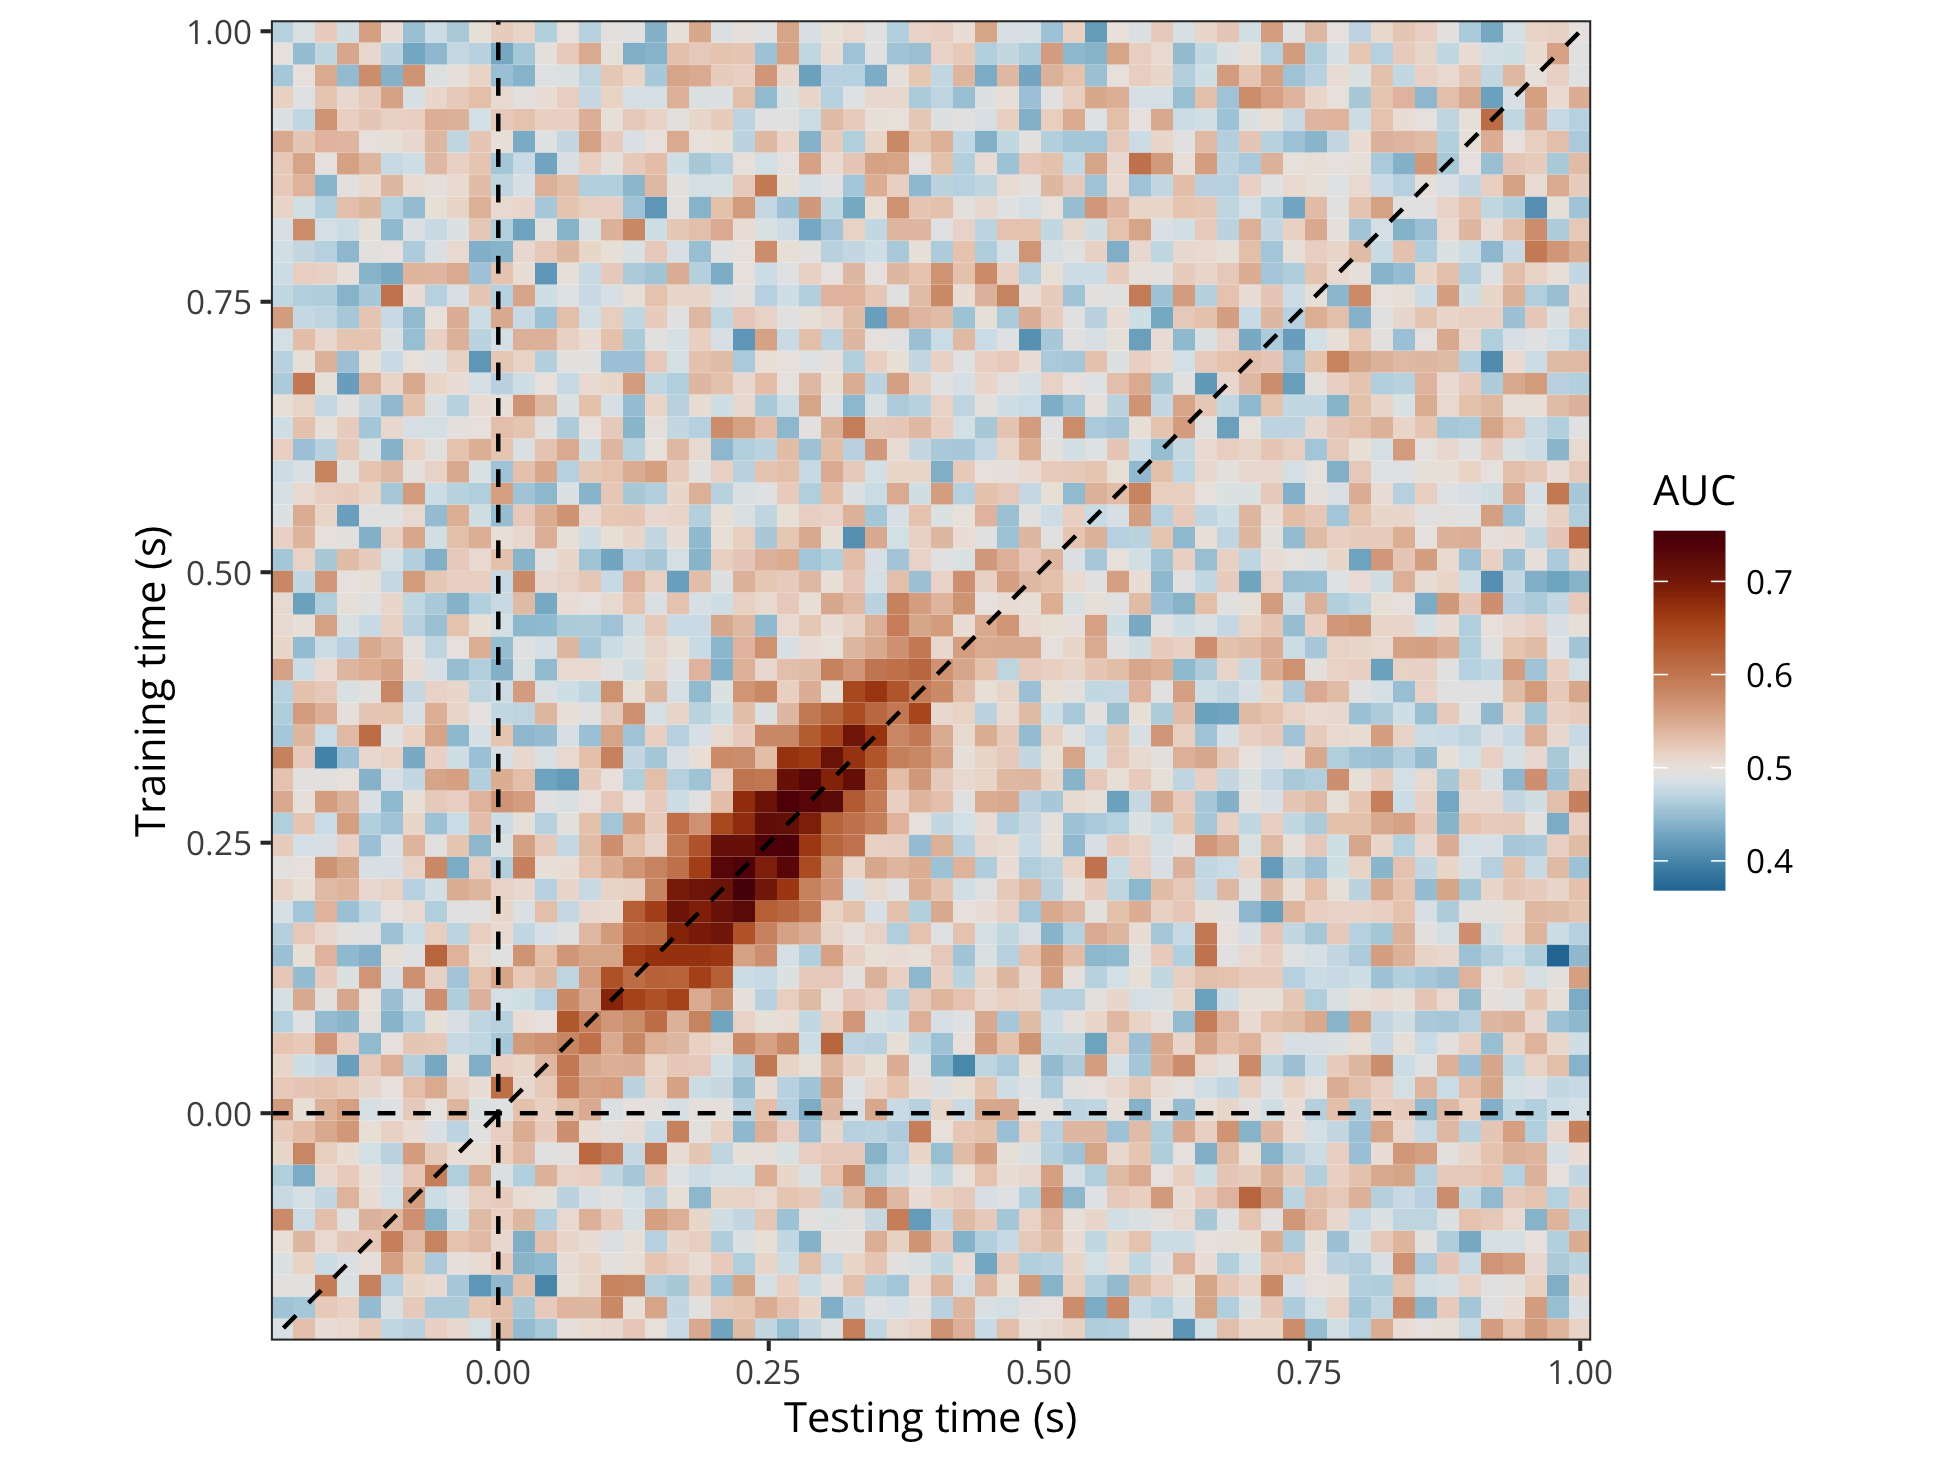
\includegraphics[width=0.75\textwidth,height=\textheight]{brms_meeg_files/figure-pdf/fig-sim-timegen-1.png}

}

\end{figure}%

To model cross-temporal generalisation matrices of decoding performance
(ROC AUC), we extended the initial (decoding) GAM to take into account
the bivariate temporal distribution of AUC values, thus producing
naturally smoothed estimates (timecourses) of AUC values and posterior
probabilities. This model can be written as follows:

\[
\begin{aligned}
\text{AUC}_{i} &\sim \mathrm{Beta}(\mu_{i}, \phi)\\
g(\mu_{i}) &= f \left(\text{train}_{i}, \text{test}_{i} \right)\\
\end{aligned}
\]

where we assume that AUC values come from a \(\mathrm{Beta}\)
distribution with two parameters \(\mu\) and \(\phi\). We can think of
\(f \left(\text{train}_{i}, \text{test}_{i} \right)\) as a surface (a
smooth function of two variables) that we can model using a
2-dimensional splines. Let
\(\mathbf{s}_{i} = \left(\text{train}_{i}, \text{test}_{i} \right)\) be
some pair of training and testing samples, and let
\(\mathbf{k}_{m} = \left(\text{train}_{m}, \text{test}_{m} \right)\)
denote the \(m^{\text{th}}\) knot in the domain of \(\text{train}_{i}\)
and \(\text{test}_{i}\). We can then express the smooth function as:

\[
f \left(\text{train}_{i}, \text{test}_{i} \right) = \alpha + \sum_{m=1}^M \beta_{m} b_{m} \left(\tilde{s}_{i}, \tilde{k}_{m} \right)
\]

Note that \(b_{m}(,)\) is a basis function that maps
\(R \times R \rightarrow R\). A popular bivariate basis function uses
\emph{thin-plate splines} (\citeproc{ref-wood2003}{Wood, 2003}), which
extend to \(\mathbf{s}_{i} \in \mathbb{R}^{d}\) and \(\partial l_{g}\)
penalties. These splines are designed to interpolate and approximate
smooth surfaces over two dimensions (hence the ``bivariate'' term). For
\(d=2\) dimensions and \(l=2\) (smoothness penalty involving second
order derivative):

\[
f \left(\tilde{s}_{i} \right) = \alpha + \beta_{1} x_{i} + \beta_{2} z_{i} +\sum_{m=1}^{M} \beta_{2+m} b_m\left(\tilde{s}_i, \tilde{k}_m\right)
\]

using the the radial basis function given by:

\[
b_m\left(\tilde{s}_i, \tilde{k}_m\right)=\left\|\tilde{s}_i-\tilde{k}_m\right\|^2 \log \left\|\tilde{s}_i-\tilde{k}_m\right\|
\]

where \(\left\|\mathbf{s}_i-\mathbf{k}_{m}\right\|\) is the Euclidean
distance between the covariate \(\mathbf{s}_{i}\) and the knot location
\(\mathbf{k}_{m}\). We fitted this model using \texttt{brms}\ldots{}

\begin{Shaded}
\begin{Highlighting}[]
\CommentTok{\# fitting a GAM with two temporal dimensions}
\NormalTok{timegen\_gam }\OtherTok{\textless{}{-}} \FunctionTok{brm}\NormalTok{(}
    \CommentTok{\# 2D thin{-}plate spline (tp)}
    \CommentTok{\# auc \textasciitilde{} t2(train\_time, test\_time, bs = "tp", k = 10),}
\NormalTok{    auc }\SpecialCharTok{\textasciitilde{}} \FunctionTok{t2}\NormalTok{(train\_time, test\_time, }\AttributeTok{bs =} \StringTok{"tp"}\NormalTok{, }\AttributeTok{k =} \DecValTok{20}\NormalTok{),}
    \AttributeTok{data =}\NormalTok{ timegen\_data,}
    \AttributeTok{family =} \FunctionTok{Beta}\NormalTok{(),}
    \AttributeTok{warmup =} \DecValTok{2000}\NormalTok{,}
    \AttributeTok{iter =} \DecValTok{5000}\NormalTok{,}
    \AttributeTok{chains =} \DecValTok{8}\NormalTok{,}
    \AttributeTok{cores =} \DecValTok{8}\NormalTok{,}
    \CommentTok{\# file = "models/timegen\_gam\_t2.rds" \# k = 10}
    \AttributeTok{file =} \StringTok{"models/timegen\_gam\_t2\_k20.rds"} \CommentTok{\# k = 20}
\NormalTok{    )}
\end{Highlighting}
\end{Shaded}

\begin{figure}[H]

\caption{Simulated data with thresholds derived from the BGAM (left),
predicted AUC values (middle), and ratios of posterior probabilies of
decoding accuracy being above chance level (right) according to the
bivariate BGAM (for k=10, top row, and k=20, bottom row).}

{\centering 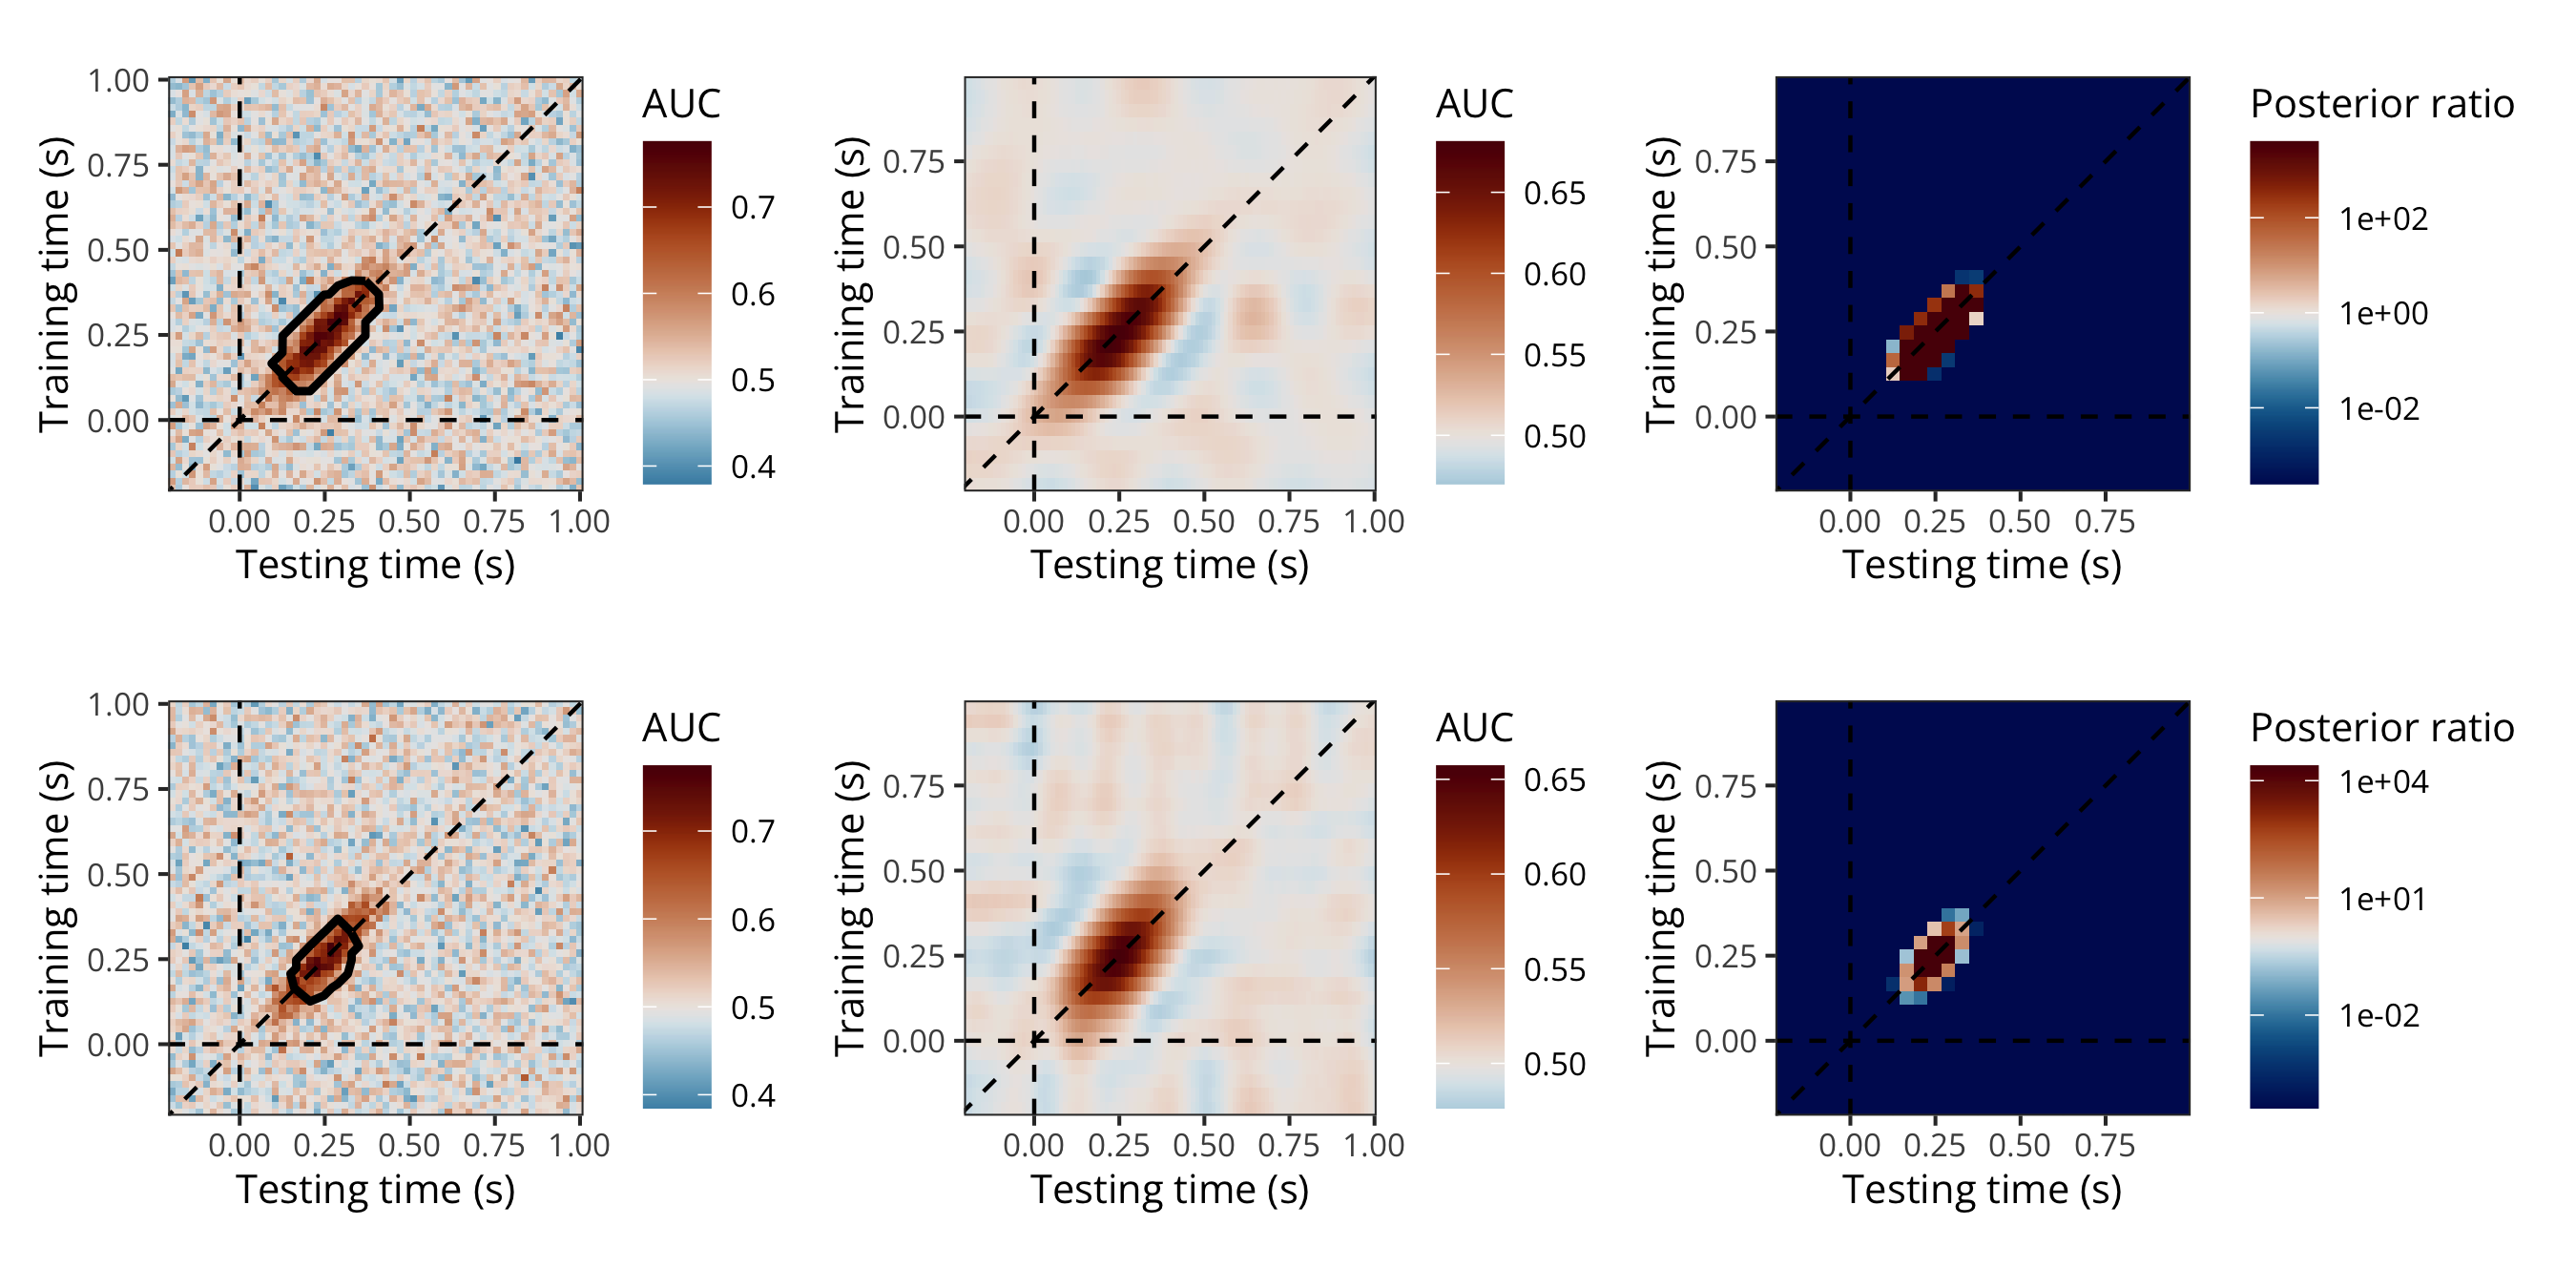
\includegraphics[width=1\textwidth,height=\textheight]{brms_meeg_files/figure-pdf/gam-timegen-post-preds-1.png}

}

\end{figure}%

Could be extended to spatial and temporal dimensions with formulas such
as \texttt{te(x,\ y,\ Time,\ d\ =\ c(2,\ 1)\ )}\ldots{}

\newpage

\section{Alternative to GAMs: Approximate Gaussian Process
regression}\label{alternative-to-gams-approximate-gaussian-process-regression}

A Gaussian process (GP) is a stochastic process that defines the
distribution over a collection of random variables indexed by a
continuous variable, that is \(\{f(t): t \in \mathcal{T}\}\) for some
index set \(\mathcal{T}\) (\citeproc{ref-rasmussen2005}{Rasmussen \&
Williams, 2005};
\citeproc{ref-riutort-mayol_practical_2023}{Riutort-Mayol et al.,
2023}). Whereas Bayesian linear regression outputs a distribution over
the parameters of some predefined parametric model, the GP approach, in
contrast, is a non-parametric approach, in that it finds a distribution
over the possible functions that are consistent with the observed data.
However, note that nonparametric does not mean there aren't parameters,
it means that there are infinitely many parameters.

From
\href{https://www.rdocumentation.org/packages/brms/versions/2.22.0/topics/gp}{brms
documentation}: A GP is a stochastic process, which describes the
relation between one or more predictors
\(x=\left(x_{1}, \ldots, x_{d}\right)\) and a response \(f(x)\), where
\(d\) is the number of predictors. A GP is the generalization of the
multivariate normal distribution to an infinite number of dimensions.
Thus, it can be interpreted as a prior over functions. The values of
\(f()\) at any finite set of locations are jointly multivariate normal,
with a covariance matrix defined by the covariance kernel
\(k_p\left(x_i, x_j\right)\), where \(p\) is the vector of parameters of
the GP:

\[
\left(f\left(x_{1}\right), \ldots f\left(x_{n}\right) \sim \operatorname{MVN}\left(0, \left(k_p\left(x_{i}, x_{j}\right)\right)_{i, j=1}^{n}\right)\right.
\]

The smoothness and general behaviour of the function \(f\) depends only
on the choice of covariance kernel, which ensures that values that are
close together in the input space will be mapped to similar output
values\ldots{}

From this perspective, \(f\) is a realisation of an infinite dimensional
normal distribution:

\[
f \sim \mathrm{Normal}(0, C(\lambda))
\]

where \(C\) is a covariance kernel with hyperparameters \(\lambda\) that
defines the covariance between two function values \(f\left(t_1\right)\)
and \(f\left(t_2\right)\) for two time points \(t_1\) and \(t_2\)
(\citeproc{ref-rasmussen2005}{Rasmussen \& Williams, 2005}). Similar to
the different choices of the basis function for splines, different
choices of the covariance kernel lead to different GPs. In this article,
we consider the squared-exponential (a.k.a. radial basis function)
kernel, which computes the squared distance between points and converts
it into a measure of similarity. It is defined as:

\[
C(\lambda) := C\left(t_1, t_2, \sigma, \gamma\right) := \sigma^2 \exp \left(-\frac{||t_1-t_2||^{2}}{2 \gamma^2}\right)
\]

with hyperparameters \(\lambda = (\sigma, \gamma)\), expressing the
overall scale of GP and the length-scale, respectively
(\citeproc{ref-rasmussen2005}{Rasmussen \& Williams, 2005}). The
advantages of this kernel are that it is computationally efficient and
(infinitely) smooth making it a reasonable choice for the purposes of
the present article. Here again, \(\lambda\) hyperparameters are
estimated from the data, along with all other model parameters.

Taken from
\url{https://michael-franke.github.io/Bayesian-Regression/practice-sheets/10c-Gaussian-processes.html}:
For a given vector \(\mathbf{x}\), we can use the kernel to construct
finite multi-variate normal distribution associated with it like so:

\[
\mathbf{x} \mapsto_{G P} \operatorname{MVNormal}(m(\mathbf{x}), k(\mathbf{x}, \mathbf{x}))
\]

where \(m\) is a function that specifies the mean for the distribution
associated with \(\mathbf{x}\). This mapping is essentially the Gaussian
process: a systematic association of vectors of arbitrary length with a
suitable multi-variate normal distribution.

Low-rank approximate Gaussian processes are of main interest in machine
learning and statistics due to the high computational demands of exact
Gaussian process models
(\citeproc{ref-riutort-mayol_practical_2023}{Riutort-Mayol et al.,
2023})\ldots{}

\newpage

\section{How to choose the GAM basis dimension?}\label{sec-basis}

Here provide recommendation about how to define \texttt{k}. An option is
to vary \texttt{k} and examine the predictions and posterior predictive
checks (PPCs) of each model\ldots{} In this example
(Figure~\ref{fig-choose-k})\ldots{} However, it is not possible to
provide general recommendations, as the optimal \texttt{k} depends on
the sampling rate, the preprocessing steps (e.g., signal-to-noise ratio,
low-pass filtering, etc), and the neural dynamics of the phenomenon
under study.

\begin{figure}[!htb]

\caption{\label{fig-choose-k}Posterior predictions and posterior
predictive checks for the GAM with varying k (in rows).}

\centering{

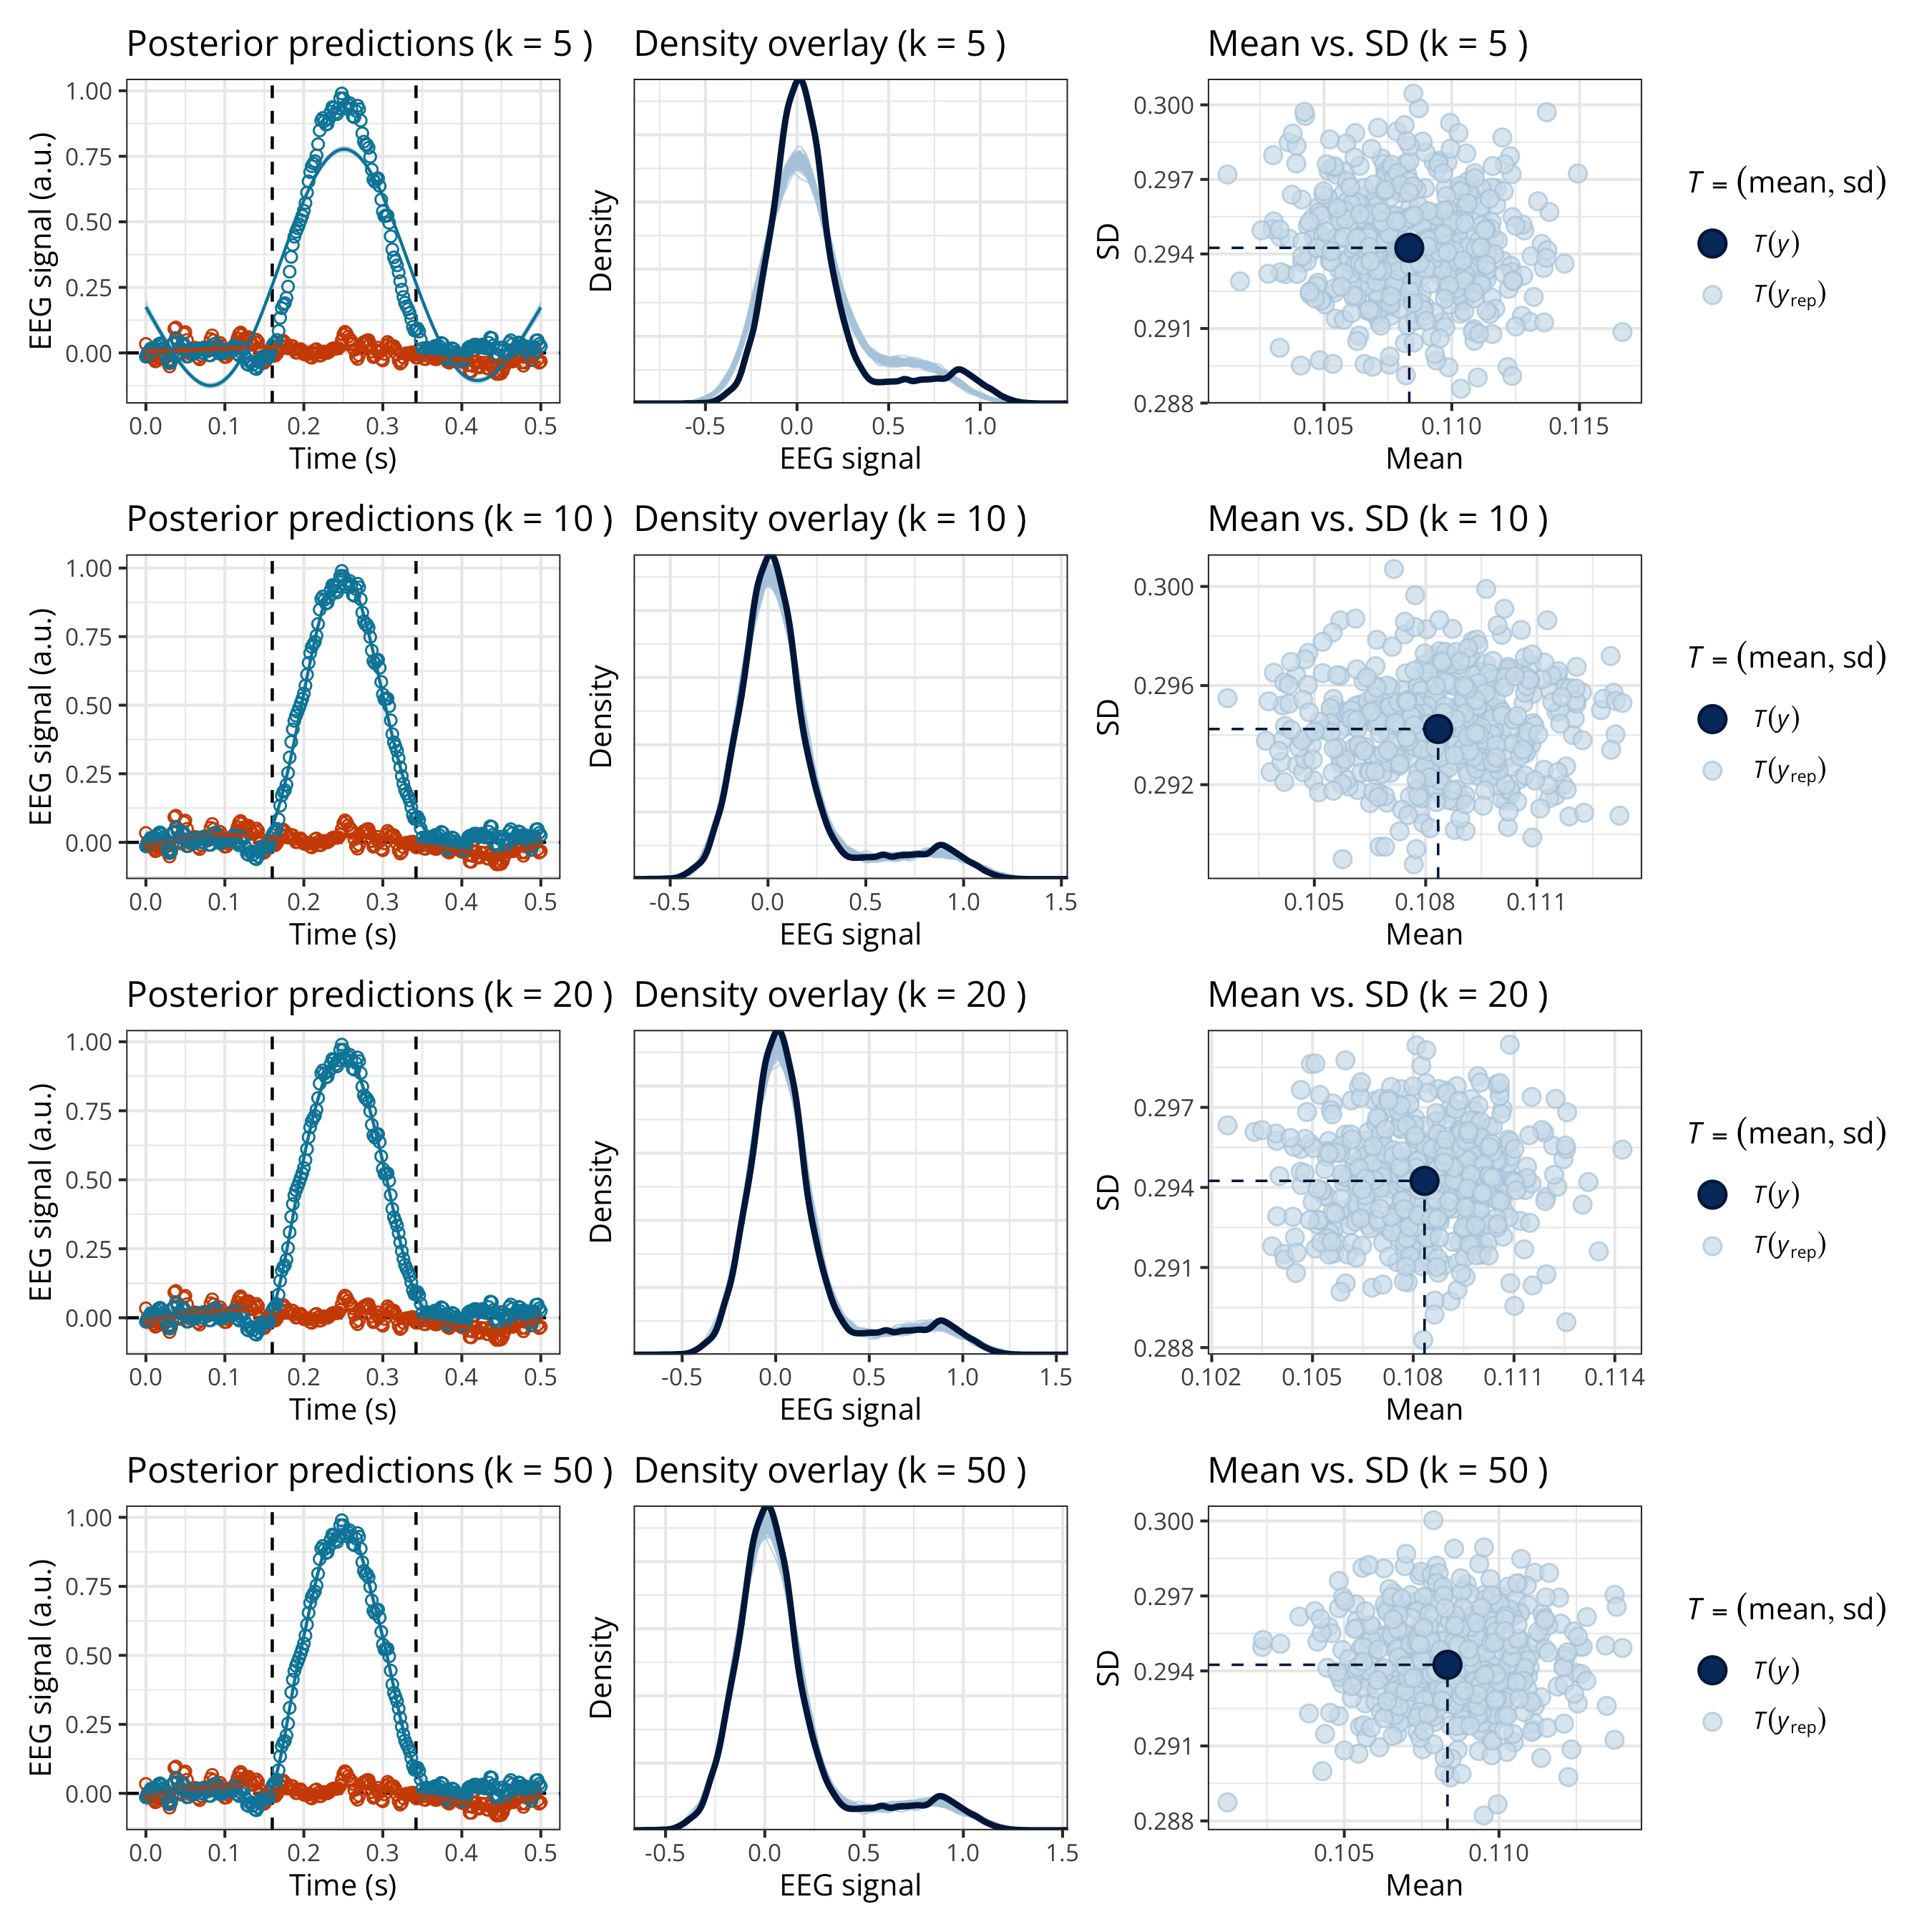
\includegraphics[width=1\textwidth,height=\textheight]{brms_meeg_files/figure-pdf/fig-choose-k-1.png}

}

\end{figure}%

\newpage

\section{\texorpdfstring{\texttt{R} package and integration with
\texttt{MNE-Python}}{R package and integration with MNE-Python}}\label{r-package-and-integration-with-mne-python}

For users who are already familiar with \texttt{brms}, the recommended
pipeline is to import ERPs or decoding results in \texttt{R} and analyse
these data using the code provided in the main paper. However, it is
also possible to call functions from the \texttt{neurogam\ R} package
(available at \url{https://github.com/lnalborczyk/neurogam}), which come
with sensible defaults.

\begin{Shaded}
\begin{Highlighting}[]
\CommentTok{\# installing (if needed) and loading the neurogam R package}
\CommentTok{\# remotes::install\_github("https://github.com/lnalborczyk/neurogam")}
\FunctionTok{library}\NormalTok{(neurogam)}

\CommentTok{\# using the testing\_through\_time() function from the neurogam package}
\CommentTok{\# this may take a few minutes (or hours depending the machine\textquotesingle{}s}
\CommentTok{\# performance and data size)...}
\NormalTok{gam\_onset\_offset }\OtherTok{\textless{}{-}} \FunctionTok{testing\_through\_time}\NormalTok{(}
    \CommentTok{\# dataframe with M/EEG data in long format}
    \AttributeTok{data =}\NormalTok{ raw\_df,}
    \CommentTok{\# threshold for defining clusters (20 by default)}
    \AttributeTok{threshold =} \DecValTok{20}\NormalTok{,}
    \CommentTok{\# the *\_id arguments are used to specify the relevant columns in data }
    \AttributeTok{participant\_id =} \StringTok{"participant"}\NormalTok{, }\AttributeTok{meeg\_id =} \StringTok{"eeg"}\NormalTok{,}
    \AttributeTok{time\_id =} \StringTok{"time"}\NormalTok{, }\AttributeTok{predictor\_id =} \StringTok{"condition"}\NormalTok{,}
    \CommentTok{\# number of warmup MCMC iterations}
    \AttributeTok{warmup =} \DecValTok{1000}\NormalTok{,}
    \CommentTok{\# total number of MCMC iterations}
    \AttributeTok{iter =} \DecValTok{5000}\NormalTok{,}
    \CommentTok{\# number of MCMCs}
    \AttributeTok{chains =} \DecValTok{4}\NormalTok{,}
    \CommentTok{\# number of parallel cores to use for running the MCMCs}
    \AttributeTok{cores =} \DecValTok{4}
\NormalTok{    )}

\CommentTok{\# displaying the results}
\NormalTok{gam\_onset\_offset}\SpecialCharTok{$}\NormalTok{clusters}
\end{Highlighting}
\end{Shaded}

The \texttt{neurogam} package can also be called from \texttt{Python}
using the \texttt{rpy2} module, and can easily be integrated into
\texttt{MNE-Python} pipelines. For example, we use it below to estimate
the onset and offset of effects for one EEG channel from a MNE evoked
object. Note that the code used to reshape the \texttt{sample\ MNE}
dataset is available in the online supplementary materials, and we refer
to the
\href{https://mne.tools/stable/auto_tutorials/epochs/50_epochs_to_data_frame.html}{MNE
documentation} about converting \texttt{MNE} epochs to \texttt{Pandas}
dataframes in long format (i.e., with one observation per row).

\begin{Shaded}
\begin{Highlighting}[]
\CommentTok{\# loading the Python modules}
\ImportTok{import}\NormalTok{ rpy2.robjects }\ImportTok{as}\NormalTok{ robjects}
\ImportTok{from}\NormalTok{ rpy2.robjects.packages }\ImportTok{import}\NormalTok{ importr}
\ImportTok{from}\NormalTok{ rpy2.robjects }\ImportTok{import}\NormalTok{ pandas2ri}
\ImportTok{from}\NormalTok{ rpy2.robjects.conversion }\ImportTok{import}\NormalTok{ localconverter}

\CommentTok{\# importing the "neurogam" R package}
\NormalTok{neurogam }\OperatorTok{=}\NormalTok{ importr(}\StringTok{"neurogam"}\NormalTok{)}

\CommentTok{\# activating automatic pandas{-}R conversion}
\NormalTok{pandas2ri.activate()}

\CommentTok{\# assuming reshaped\_df is some M/EEG data reshaped in long format}
\ControlFlowTok{with}\NormalTok{ localconverter(robjects.default\_converter }\OperatorTok{+}\NormalTok{ pandas2ri.converter):}
    
\NormalTok{    reshaped\_df\_r }\OperatorTok{=}\NormalTok{ robjects.conversion.py2rpy(reshaped\_df)}
    

\CommentTok{\# using the testing\_through\_time() function from the neurogam R package}
\NormalTok{gam\_onset\_offset }\OperatorTok{=}\NormalTok{ neurogam.testing\_through\_time(}
\NormalTok{    data}\OperatorTok{=}\NormalTok{reshaped\_df\_r,}
\NormalTok{    threshold}\OperatorTok{=}\DecValTok{10}\NormalTok{,}
\NormalTok{    multilevel}\OperatorTok{=}\VariableTok{False}
\NormalTok{    )}

\CommentTok{\# displaying the results}
\BuiltInTok{print}\NormalTok{(}\BuiltInTok{list}\NormalTok{(gam\_onset\_offset) )}
\end{Highlighting}
\end{Shaded}







\end{document}
